\documentclass[11pt,a4paper]{article}
\usepackage[spanish,es-noshorthands,es-nodecimaldot,es-tabla,es-noindentfirst,es-nosectiondot]{babel}
\addto\captionsspanish{\renewcommand{\figurename}{Figura}}
\usepackage{fontspec}
\IfFontExistsTF{texgyrepagella-regular.otf}
  {\setmainfont{texgyrepagella}[Extension=.otf,UprightFont=*-regular,BoldFont=*-bold,
    ItalicFont=*-italic,BoldItalicFont=*-bolditalic]}
  {\IfFontExistsTF{Palatino Linotype}{\setmainfont{Palatino Linotype}}{\setmainfont{Latin Modern Roman}}}
\usepackage{amsmath,amssymb,amsthm}
\usepackage{unicode-math}
\setmathfont{latinmodern-math.otf}
\AtBeginDocument{\let\setminus\smallsetminus}
\usepackage[margin=26mm]{geometry}
\usepackage{microtype}
\usepackage[nobottomtitles*]{titlesec}
\renewcommand{\bottomtitlespace}{.12\textheight}
\usepackage{array,booktabs,longtable}
\newcolumntype{L}[1]{>{\raggedright\arraybackslash}p{#1}}
\usepackage{xcolor}
\usepackage{tikz}
\definecolor{btinta}{HTML}{223B49}
\definecolor{bgris}{HTML}{DDE6E7}
\definecolor{bpapel}{HTML}{FFFFFF}
\newcommand{\bcuadricula}[1]{\btablerobase{#1}{1}}
\newcommand{\bcuadriculacero}[1]{\btablerobase{#1}{0}}
\newcommand{\btablerobase}[2]{%
  \fill[bpapel] (0,0) rectangle (#1,#1);
  \foreach \r in {1,...,#1}{%
    \foreach \c in {1,...,#1}{%
      \ifodd\numexpr\r+\c\relax
        \fill[bgris] (\c-1,#1-\r) rectangle (\c,#1-\r+1);
      \fi
    }
    \pgfmathtruncatemacro{\bnum}{\r-1+#2}
    \node[font=\scriptsize,anchor=east] at (-.10,#1-\r+.5) {\bnum};
    \node[font=\scriptsize,anchor=south] at (\r-.5,#1+.06) {\bnum};
  }
  \foreach \t in {0,...,#1}{\draw[black!45,line width=.3pt] (\t,0)--(\t,#1) (0,\t)--(#1,\t);}
  \draw[btinta,line width=.6pt] (0,0) rectangle (#1,#1);
}
\newcommand{\breina}[3]{%
  \begin{scope}[shift={(#3-.5,#1-#2+.50)}]
    \fill[bpapel] (0,0) circle[radius=.36];
    \fill[btinta] (-.29,.15)--(-.13,.04)--(0,.30)--(.13,.04)--(.29,.15)--(.18,-.15)--(-.18,-.15)--cycle;
    \fill[btinta] (-.21,-.22) rectangle (.21,-.18);
  \end{scope}
}
\newcommand{\bmarca}[3]{\fill[btinta!62] (#3-.5,#1-#2+.50) circle[radius=.055];}

\usepackage[unicode,colorlinks=true,linkcolor={blue!45!black},citecolor={green!35!black},
  urlcolor={blue!55!black}]{hyperref}
\linespread{1.05}
\setlength{\parindent}{1.15em}
\setlength{\parskip}{0pt plus .35pt}
\setlength{\textfloatsep}{14pt plus 3pt minus 3pt}
\setlength{\intextsep}{12pt plus 3pt minus 3pt}
\setlength{\abovecaptionskip}{6pt}
\setlength{\belowcaptionskip}{2pt}
\AtBeginDocument{\setlength{\abovedisplayskip}{9pt plus 2pt minus 3pt}%
  \setlength{\belowdisplayskip}{9pt plus 2pt minus 3pt}}
\clubpenalty=7000
\widowpenalty=7000
\displaywidowpenalty=3000
\setlength{\emergencystretch}{2em}
\allowdisplaybreaks[2]
\setlength{\tabcolsep}{4pt}
\renewcommand{\arraystretch}{1.12}
\newcommand{\cerr}{c_{\mathrm{err}}}
\newcommand{\status}[1]{\textnormal{\textsf{[#1]}}}

\newtheorem{teorema}{Teorema}[section]
\newtheorem{proposicion}[teorema]{Proposición}
\newtheorem{lema}[teorema]{Lema}
\newtheorem{corolario}[teorema]{Corolario}

\hypersetup{pdfauthor={Dilan Steven Mejia},pdftitle={El término de orden 1/n del problema de las n reinas},
 pdfsubject={Enumeración asintótica; error con signo del predictor canónico},pdflang={es}}
\title{El término de orden $1/n$ del problema de las $n$ reinas}
\author{Dilan Steven Mejia\thanks{\href{mailto:mejiadilan@hotmail.com}{\nolinkurl{mejiadilan@hotmail.com}}}}
\date{}
\begin{document}
\maketitle
\begin{abstract}\phantomsection\label{sec:resumen}
\noindent Sea \(Q(n)\) el número de formas de colocar \(n\) reinas sin ataques mutuos en un tablero
de \(n\times n\). El predictor canónico \(Q_{\rm pred}(n)\), una fórmula finita construida a partir del
maximizador de una entropía en el tablero, reproduce el término principal y la
constante de \(\log Q(n)\); ambos hechos proceden de preprints anteriores del autor. Determinamos ahora la
primera corrección al predictor finito:
el error con signo \(R_Q(n)=\log\bigl(Q(n)/Q_{\rm pred}(n)\bigr)\) satisface
\(nR_Q(n)\to\cerr\). Damos una fórmula explícita para este límite y obtenemos
\(Q(n)/Q_{\rm pred}(n)=1+\cerr/n+o(1/n)\).

\smallskip\noindent
Para obtener la fórmula elegimos una solución uniformemente al azar y revelamos sus filas en orden
aleatorio. El límite reúne una corrección inicial, la integral del defecto medio que deja cada
inserción y tres contribuciones del tablero que queda al detener el proceso: la de las torres, la de
un par de casillas en una misma diagonal y la de la interacción de las dos diagonales de un
cuadrado. Comparar dos niveles de parada da el límite y prueba que la integral converge
absolutamente. La demostración se apoya en resultados de esos preprints y está asistida por ordenador en
dos pasos.

\smallskip\noindent
La evaluación numérica de la fórmula da \(\cerr\approx0{,}40550038\), con una estimación empírica del
error de \(3\cdot10^{-8}\) y una banda conservadora \(0{,}4055004\pm2\cdot10^{-7}\). Son estimaciones
numéricas y no intervalos certificados: el signo y los decimales de \(\cerr\) siguen pendientes de
certificación.

\medskip\noindent
\textbf{Palabras clave:} problema de las $n$ reinas; enumeración asintótica; permanentes;
problema de torres; aritmética de intervalos.

\noindent
\textbf{MSC 2020:} 05A16; 60C05; 15A15.
\end{abstract}

\section{Introducción}
El problema de las $n$ reinas pregunta cuántas maneras hay de colocar $n$ reinas en un tablero de
$n\times n$ sin que dos se ataquen. Denotamos ese número por $Q(n)$ y contamos por separado las
soluciones relacionadas por una simetría. Numeramos filas y columnas desde uno, con filas de arriba
abajo y columnas de izquierda a derecha, y $(i,j)$ es la casilla de la fila $i$ y la columna $j$.
Leer las columnas de las reinas por orden de filas identifica cada solución con una permutación
$\sigma$, cuyas reinas ocupan las casillas $(i,\sigma(i))$. Las restricciones diagonales piden que
las diferencias $i-\sigma(i)$ sean distintas entre sí, y también las sumas $i+\sigma(i)$; así
determinan cuáles de las $n!$ permutaciones sirven. Por ejemplo, $(2,4,1,3)$ y $(3,1,4,2)$ son las
dos soluciones del tablero de $4\times4$.

Para estudiar cómo crece $Q(n)$, conviene tomar logaritmos. Entre los antecedentes combinatorios
figuran la cota superior de Luria~\cite{luria}, la inferior de Luria y Simkin~\cite{ls} y el
trabajo de Bowtell y Keevash~\cite{bk}; juntos resuelven una conjetura de Rivin, Vardi y
Zimmermann~\cite{rvz} sobre el crecimiento de $Q(n)$. Bell y Stevens~\cite{bs} dan una visión de conjunto.
La fórmula variacional de Simkin~\cite{simkin} determina $\log Q(n)$ hasta un error $o(n)$.
En la normalización del perfil variacional~\cite{pv}, el término principal es $\log(n!)+n\Phi$.
Simkin escribe $Q(n)=((1+o(1))ne^{-\alpha})^n$ con $1{,}94<\alpha<1{,}9449$; como
$\log(n!)=n\log n-n+O(\log n)$, las dos normalizaciones se relacionan por $\Phi=1-\alpha$.
Nobel, Agrawal y Boyd~\cite{nab} obtuvieron cotas numéricas para la constante de primer orden.
Más allá del intervalo enumerado, se han obtenido estimaciones numéricas del crecimiento de $Q(n)$ por
conteo de Monte Carlo~\cite{zm} y, recientemente, por integración termodinámica de un modelo de gas
reticular~\cite{llw}.
El perfil describe la distribución de masa en el tablero y sobre cada diagonal. Estos datos
entran en el predictor canónico $Q_{\rm pred}(n)$ de~\cite{pc}. A partir de los pesos de las casillas
se calcula una entropía y se añade una corrección por la dependencia entre las líneas. El
Apéndice~\ref{app:predictor} da la fórmula finita que usamos en todo el artículo.

El siguiente avance fue identificar el término constante. Después de restar $\log(n!)+n\Phi$,
el logaritmo del predictor tiende a $C_{\rm pred}$~\cite{pc}. El conteo exacto tiene esa misma
constante~\cite{tc}. Por tanto, al formar la diferencia con signo
\[
 R_Q(n)=\log Q(n)-\log Q_{\rm pred}(n),
\]
se cancelan tanto el término principal como la constante. Un paso previo del presente trabajo,
mediante estimaciones de magnitud, da $|R_Q(n)|\le C/n$ para $n$ suficientemente grande.
El Lema~\ref{lem:previa} prueba esa cota a un solo corte fijo, bajo la ley adaptativa, que revela las
filas en orden aleatorio y elige cada reina con probabilidad proporcional al predictor del tablero
resultante (Sección~\ref{sec:signedmap}).
El Apéndice~\ref{app:signed} la usa al desarrollar la identidad de historias detenidas.
Así, $nR_Q(n)$ está acotado, aunque todavía podría oscilar con el tamaño del tablero. ¿Converge?
El Teorema~\ref{teo:principal} identifica ese límite, que denotamos por \(\cerr\). Mientras que
\(C_{\rm pred}\) es el término constante que comparten los dos logaritmos, \(\cerr/n\) es la primera
corrección relativa al pasar del predictor finito al conteo exacto. Si se quisiera desarrollar
directamente \(\log Q(n)\) respecto de \(\log(n!)+n\Phi+C_{\rm pred}\), habría que sumar a
\(\cerr\) el coeficiente de \(1/n\) del propio \(\log Q_{\rm pred}(n)\), si ese coeficiente existe.

\paragraph{En qué se apoya la demostración.} La demostración del Teorema~\ref{teo:principal} no es
autocontenida. Usa la existencia y la regularidad del perfil variacional~\cite{pv}, el corte temprano
de~\cite{ef}, los teoremas de inserción y de consistencia del predictor~\cite{pc}, y la regla de parada,
la permanencia y las cotas estáticas en que se basa el término constante~\cite{tc}. Estos cuatro
trabajos son preprints del autor; cada registro de Zenodo contiene el original en español y una versión
en inglés. La Sección~\ref{sec:importados} enumera los enunciados que se usan, con sus hipótesis, e
indica los dos lugares en que se toma un argumento de una demostración y no sólo de un enunciado. Dos
pasos están asistidos por ordenador, en aritmética racional exacta (Apéndice~\ref{app:pair}). El valor
numérico de \(\cerr\) es una estimación y no forma parte del teorema.

La dificultad se ve al revelar una solución fila por fila. Mientras quedan muchas filas, cada
inserción introduce un defecto pequeño y es su suma con signo la que importa. Al quedar pocas
filas, dos casillas aún disponibles pueden compartir una diagonal. Los resultados de completabilidad
de~\cite{ef} describen el papel de las últimas filas;
Glock, Munhá Correia y Sudakov~\cite{gms} estudiaron cuándo puede completarse una colocación
parcial. Para calcular el coeficiente necesitamos además el peso de esos conflictos en el error.
Siguiendo el corte temprano de~\cite{ef}, detenemos el proceso cuando queda una fracción fija
de filas vacías. Esto permite estudiar el defecto acumulado antes del corte y medir el error en
el tablero residual. La comparación de dos cortes reunirá ambas contribuciones.
La Figura~\ref{fig:mascara-ilustrada} sigue la primera solución de cuatro reinas: al revelar una
sola reina ya se ve la diferencia entre una completación de torres y una de reinas.
\begin{figure}[htbp]
\centering
\begin{tikzpicture}[x=.61cm,y=.61cm]
  \bcuadricula{4}
  \foreach \r/\c in {1/2,2/4,3/1,4/3}{\breina{4}{\r}{\c}}
  \node[font=\small] at (2,-.62) {Solución completa};
  \begin{scope}[shift={(7,0)}]
    \bcuadricula{4}
    \fill[orange,opacity=.24] (0,3) rectangle (4,4);
    \fill[blue,opacity=.15] (1,0) rectangle (2,4);
    \begin{scope}
      \clip (0,0) rectangle (4,4);
      \draw[teal!75!black,line width=.7pt] (-2,7)--(6,-1);
      \draw[red!70!black,dashed,line width=.7pt] (-2,0)--(6,8);
    \end{scope}
    \foreach \r/\c in {2/4,3/1,3/3,4/1,4/3,4/4}{\bmarca{4}{\r}{\c}}
    \breina{4}{1}{2}
    \node[font=\small] at (2,-.62) {Una reina revelada};
  \end{scope}
  \begin{scope}[shift={(14,.1)}]
    \foreach \r/\cells in {1/{0,0,1},2/{1,1,0},3/{1,1,1}}{
      \foreach \w [count=\c] in \cells {
        \ifnum\w=1 \fill[teal!16] (\c-1,3-\r) rectangle (\c,4-\r);\fi
        \node[font=\small] at (\c-.5,3.5-\r) {$\w$};
      }
    }
    \draw[step=1,black!45,line width=.3pt] (0,0) grid (3,3);
    \draw[btinta,line width=.6pt] (0,0) rectangle (3,3);
    \foreach \i/\r in {1/2,2/3,3/4}{\node[font=\scriptsize] at (-.3,3.5-\i) {$\r$};}
    \foreach \i/\c in {1/1,2/3,3/4}{\node[font=\scriptsize] at (\i-.5,3.32) {$\c$};}
    \node[font=\small] at (1.5,-.72) {Máscara residual};
  \end{scope}
\end{tikzpicture}
\caption{De una solución al problema de torres. Tras revelar $(1,2)$, los puntos del centro
son los unos de la máscara de la derecha, con sus etiquetas originales. La fila 2 exige la
columna 4. Las filas 3 y 4 pueden repartirse las columnas 1 y 3 de dos maneras:
$\operatorname{per}M=2$. Sólo la del panel izquierdo completa las reinas. En la otra,
$(2,4)$ y $(3,3)$ se atacan. Así, $Q(B)=1$.}\label{fig:mascara-ilustrada}
\end{figure}


\section{El coeficiente del error con signo}\label{sec:principal}
En la fórmula para el límite, $\mathcal C_0$ recoge el ajuste en el tablero inicial y la suma de
los defectos de inserción hasta la parada. El término $P_0-S$ mide el error que aún queda en las
casillas disponibles en ese instante.

Sea $x$ la fracción de filas aún vacías. En $x=1$ el tablero inicial está vacío y al acercarse
$x$ a cero quedan las últimas filas. La función $d(x)$ suma dieciséis contribuciones al defecto
medio de segundo orden de una inserción del predictor~\cite{pc}. El
Apéndice~\ref{app:interior} identifica esas contribuciones. El prefactor de líneas
$\mathcal V(x)$ y la corrección de torres $F(x)$ se definen en el Apéndice~\ref{app:predictor}.
Los dos enunciados siguientes están demostrados \status{D}, dados los resultados importados en la
Sección~\ref{sec:importados} y con dos pasos asistidos por ordenador \status{O}; las etiquetas se
explican en la Sección~\ref{sec:claim-ledger}. Aquí y en lo que sigue, el \emph{perfil físico} es la
densidad $\nu_1$ de una solución completa con sus vacancias diagonales $u_f$
(Sección~\ref{sec:profile-data}); en general, \emph{físico} califica a un objeto tal como aparece en el
tablero, por oposición a los aproximantes, las continuaciones y las mallas auxiliares que se usan en la
demostración. El \emph{tablero ordinario} es el tablero usual de $n\times n$, vacío al comienzo, por
oposición a los tableros residuales de una historia (Sección~\ref{sec:importados}) y a las máscaras de
torres (Sección~\ref{sec:torres}); es el uso de~\cite{pc,tc}.

\begin{teorema}[Teorema principal]\label{teo:principal}
Para el tablero ordinario existe el límite
\begin{align}
 \cerr&=\lim_{n\to\infty}nR_Q(n)=\mathcal C_0+P_0-S,\label{eq:main}\\
 \mathcal C_0&=F(1)-\tfrac1{12}+\int_0^1 \frac{\numerr(x)}{x^2}\,dx,\notag\\
 \numerr(x)&=d(x)+G(x)-xG'(x),\qquad G(x)=\mathcal V(x)+F(x)-\tfrac1{12},\notag\\
 P_0&=P_T+J,\qquad J=-B_2+L_2,\notag
\end{align}
y la integral de~\eqref{eq:main} converge absolutamente.
\end{teorema}
En la máscara llena el núcleo de torres escalado es constante, de modo que \(F(1)=0\)
(sección~\ref{sec:profile-data}). Los términos se definen así: $d$ en~\eqref{eq:d-suma}; $F$ y
$\mathcal V$ en~\eqref{eq:F-def} y~\eqref{eq:V-def}; $P_T=\lim_{b\downarrow0}P_T(b)$ con $P_T(b)$ como
en~\eqref{eq:pt-frontera-fija}; $B_2$ y $L_2$ en~\eqref{eq:J-def}, mediante los funcionales de estado
de~\eqref{eq:estado-def}; y $S$ en~\eqref{eq:S-def}. Aquí $P_T$ es la contribución de torres en la
llegada. Para obtener
 $B_2$ y $L_2$ a partir del
camino de pesos de un par colineal, se suman las dos orientaciones. En cada orientación se
ponderan los cuatro estados de disponibilidad de los otros dos vértices.
$S$ recoge la interacción de los dos pares de un cuadrado completo.

\begin{corolario}\label{cor:derivada}
Para el perfil físico, $\numerr(0)=0$ y $\numerr'(0)=d'(0)=0$. Además,
\[
 \log Q(n)=\log Q_{\rm pred}(n)+\cerr/n+o(n^{-1}),\qquad
 Q(n)/Q_{\rm pred}(n)=1+\cerr/n+o(n^{-1}).
\]
\end{corolario}
Multiplicar el predictor por \(\exp(\cerr/n)\) deja un error relativo \(o(1/n)\).
El corolario no da un umbral a partir del cual la corrección mejore el resultado en cada tamaño.
La demostración toma la integral truncada en un corte $b>0$ fijo. La comparación de dos cortes
da su límite y de esa convergencia se deducen $\numerr(0)=0$ y $\numerr'(0)=0$ (Apéndice~\ref{app:closing}).
La Conjetura~10.1 de~\cite{pc} afirma que existen $C$ y $n_0$ tales que
$|\log Q(n)-\log Q_{\rm pred}(n)|\le C/n$ para todo $n\ge n_0$; el Lema~\ref{lem:previa} la demuestra.
El corolario identifica el coeficiente con signo dentro de esa tasa.
La demostración proporciona una expresión para el coeficiente; certificar el signo que sugiere su
evaluación todavía requiere un intervalo suficientemente estrecho.

\paragraph{Lectura de la integral lejos del extremo.} El Lema~\ref{lem:regularidad-extremo} da la
analiticidad de $G$ sólo cerca de $[0,x_0]$. En $[x_0,1]$ la demostración usa el sumando $(G-xG')/x^2$
sólo a través de su primitiva $-G(x)/x$: la identidad interior del Apéndice~\ref{app:interior} es
$\int_b^1d(x)x^{-2}\,dx+G(b)/b-G(1)$. En consecuencia, la parte de la integral de~\eqref{eq:main} sobre
$[x_0,1]$ se entiende como $\int_{x_0}^1d(x)x^{-2}\,dx+G(x_0)/x_0-G(1)$. Esto sólo requiere que $d$ sea
continua allí (Apéndice~\ref{app:interior}) y coincide con la integral clásica siempre que $G$ sea
continuamente derivable en $[x_0,1]$. La misma lectura se aplica a la descomposición de la
Sección~\ref{sec:presupuesto}.

La Sección~\ref{sec:signedmap} explica de dónde salen los signos de la fórmula. La tabla de la
Sección~\ref{sec:claim-ledger} identifica las fuentes de cada paso y el alcance de sus comprobaciones.

\section{Qué se acumula antes del corte y qué queda en la frontera}\label{sec:signedmap}
Elijamos una solución uniforme y revelemos sus reinas en un orden uniforme de las filas,
independiente de la solución. Cuando quedan \(m\) filas, el tablero residual \(B_m\) registra las
casillas disponibles. En su máscara binaria \(M_m\) cabe un problema más sencillo: colocar una
torre por fila y columna. Su conteo, \(\operatorname{per}M_m\), ya incorpora las restricciones
que imponen las piezas reveladas. Para obtener \(Q(B_m)\) falta exigir que las nuevas piezas
tampoco se ataquen entre sí por las diagonales.

Esto sugiere una primera decisión. Sean \(L\) y \(L_T\) los logaritmos de los predictores de reinas
y de torres en el tablero residual. En la parte de torres podemos usar el conteo exacto:
\[
 g_T(M)=\log\operatorname{per}M-L_T(M),\qquad L^\sharp(B)=L(B)+g_T(M).
\]
El ajuste se hace sobre la misma máscara en cada paso. Así una diferencia entre dos tableros hijos
no mezcla el error de contar torres con el coste de prohibir un ataque diagonal. En el tablero
inicial \(n g_T(M_n)\) tiende a \(F(1)-1/12\). La máscara llena es separable y \(F(1)=0\); de
aquí procede el primer sumando de~\eqref{eq:main}.

\paragraph{La suma hasta la parada.}
Fijamos los márgenes de regularidad y el parámetro macroscópico \(\delta\), y después un
\(b>0\) suficientemente pequeño. Paramos en la primera salida de la clase regular o al alcanzar
\(j=\lfloor bn\rfloor\), como en la comparación sobre historias detenidas de~\cite{tc}. Sea \(F_b\)
la llegada regular y completable a ese nivel.
En cada fila, la ley adaptativa elige una casilla con probabilidad proporcional al peso de su
tablero hijo. Si la suma de esos pesos coincidiera con el peso del padre, la recursión se
cumpliría exactamente en esa fila. El logaritmo de su cociente mide el defecto de ese paso.
Llamamos \(A^\sharp\) a la suma de estos logaritmos hasta la parada.

La solución uniforme y la ley adaptativa utilizan la misma regla de parada. Esto permite comparar
las probabilidades de una misma historia y conservar el signo de la diferencia de las salidas.
El Apéndice~\ref{app:signed} da la identidad exacta y el Apéndice~\ref{app:arrival} controla
el resto en media. A \(b\) fijo, el defecto acumulado en el interior aporta
\(\int_b^1 k(x)x^{-2}\,dx\). El Apéndice~\ref{app:interior} identifica sus dieciséis términos.

\paragraph{Lo que sobrevive en el tablero de llegada.}
Consideremos dos casillas disponibles \(e,f\) en una misma diagonal. Están en filas y columnas
distintas, de modo que dos torres podrían ocuparlas a la vez. Las otras dos posiciones del
cuadrado determinan cuatro estados. Para \(e=(r,q)\) y \(f=(r+h,q+h)\), con \(h>0\),
sean \(X\) e \(Y\) los indicadores de disponibilidad de \((r,q+h)\) y \((r+h,q)\),
respectivamente. La Figura~\ref{fig:frontera} muestra los cuatro casos.
\begin{figure}[htbp]
\centering
\begin{tikzpicture}[x=.58cm,y=.58cm]
 \foreach \dx/\sx/\sy in {0/0/0,5.8/1/0,11.6/0/1,17.4/1/1}{
  \begin{scope}[shift={(\dx,0)}]
   \bcuadricula{4}
   \draw[btinta,line width=.9pt] (1.5,3.5)--(3.5,1.5);
   \ifnum\numexpr\sx+\sy\relax=2\relax
    \draw[btinta,dash pattern=on 2pt off 1.5pt,line width=.9pt] (1.5,1.5)--(3.5,3.5);
   \fi
   \foreach \fr/\fc/\libre in {1/2/1,3/4/1,1/4/\sx,3/2/\sy}{
    \begin{scope}[shift={(\fc-.5,4.5-\fr)}]
     \fill[bpapel] (0,0) circle[radius=.26];
     \ifnum\libre=1\relax
      \draw[btinta,line width=1pt] (0,0) circle[radius=.22];
     \else
      \draw[btinta,line width=1.05pt] (-.17,-.17)--(.17,.17) (-.17,.17)--(.17,-.17);
     \fi
    \end{scope}
    \ifnum\libre=1\relax \bmarca{4}{\fr}{\fc}\fi
   }
   \node[anchor=north,font=\small] at (2,-.18) {$(X,Y)=(\sx,\sy)$};
  \end{scope}
 }
\end{tikzpicture}
\caption{Los cuatro estados del cuadrado de frontera se dibujan en una ventana de
\(4\times4\) de un tablero mayor, con coordenadas locales \(r=1\), \(q=2\), \(h=2\).
El círculo indica una casilla disponible y la cruz una vetada. La línea continua une
\(e=(1,2)\) y \(f=(3,4)\). La discontinua une \((1,4)\) con \((3,2)\) cuando ambas
están disponibles. Las demás casillas se muestran sólo como referencia. En el estado \(11\),
tras restar los efectos de cada par, los coeficientes de interacción en el logaritmo del conteo
y en el del predictor son \(-1\) y \(+2\), en unidades del producto de los cuatro pesos al orden
principal. Su diferencia \(-1-(+2)=-3\) da el signo de \(-S\) en~\eqref{eq:exceso-cuadrado}.}
\label{fig:frontera}
\end{figure}


Los cuatro casos se realizan en la solución \((1,3,5,7,2,4,6)\) del tablero de orden siete.
Antes de revelar una reina, \(X=Y=1\). Revelar \((7,6)\) veta sólo \(Y\) entre los cuatro
vértices y revelar \((4,7)\) veta sólo \(X\). Si se revelan ambas, siguen disponibles \(e,f\).

La respuesta del par marcado se evalúa con \(X,Y\) fijados. En el estado \(11\) se puede
marcar cualquiera de los dos pares diagonales, y cada uno aporta su propia respuesta. Ambos
pertenecen al mismo cuadrado, por lo que su interacción entra una sola vez en la suma sobre
cuadrados completos. Denotamos por \(B_n(b)\) la suma de las tres medias de frontera.
Al tomar \(n\to\infty\) y después \(b\downarrow0\), las dos medias sobre pares dan \(P_T\)
y \(J\), y la media de interacción da \(-S\). Los Apéndices~\ref{app:boundary}
y~\ref{app:weights} separan las contribuciones. El Apéndice~\ref{app:transfer}
efectúa el promedio de la respuesta del par bajo la ley de llegada.

\paragraph{Por qué se comparan dos cortes.}
Para \(H=P_T+J-S\), escribamos
\[
 \Phi(b)=F(1)-\tfrac1{12}+\int_b^1 k(x)x^{-2}\,dx+H.
\]
El error cumple \(\limsup_n |nR_Q(n)-\Phi(b)|\le C_\delta b+\eta(b)\), donde
\(\eta(b)=\limsup_n|B_n(b)-H|\to0\) al bajar \(b\). La constante \(C_\delta\) sirve para
todos los cortes admisibles suficientemente pequeños. Cada elección de \(b\) aproxima, por tanto,
la misma sucesión \(nR_Q(n)\). Al comparar \(b\) y \(b'\), la diferencia entre las aproximaciones
tiende a cero con los dos cortes. Así se obtiene un límite común antes de integrar hasta el
extremo. Por analiticidad y \(k(0)=0\), un término lineal de \(k\) produciría allí la divergencia
\(k'(0)\log(1/b)\). La convergencia obliga a que desaparezca. El Apéndice~\ref{app:closing}
detalla la comparación y deduce el corolario para \(d'(0)\).

La Figura~\ref{fig:cortes} ilustra los dos niveles en una historia concreta. En la prueba,
cada corte admisible da una aproximación mediante promedios sobre historias. Como ambas
aproximaciones se refieren al mismo \(nR_Q(n)\), la desigualdad triangular da
\(\lvert\Phi(b)-\Phi(b')\rvert\le C_\delta(b+b')+\eta(b)+\eta(b')\).

\begin{figure}[htbp]
\centering
\begin{tikzpicture}[x=.58cm,y=.58cm]
 \foreach \etapa/\dx in {2/0,4/10.4}{
  \begin{scope}[shift={(\dx,0)}]
   \bcuadricula{6}
   \breina{6}{1}{2}
   \breina{6}{2}{4}
   \ifnum\etapa=2\relax
    \def\casillas{3/1,3/6,4/1,4/3,5/3,5/5,6/1,6/3,6/5,6/6}
    \def\corte{b=2/3}
   \else
    \breina{6}{3}{6}
    \breina{6}{4}{1}
    \def\casillas{5/3,5/5,6/5}
    \def\corte{b'=1/3}
   \fi
   \foreach \fila/\col in \casillas{
    \draw[btinta,line width=.55pt] (\col-.5,6.5-\fila) circle[radius=.16];
    \bmarca{6}{\fila}{\col}
   }
   \draw[btinta,line width=.95pt] (0,6-\etapa)--(6,6-\etapa);
   \node[font=\small,anchor=north] at (3,-.18) {$\corte,\quad m=\the\numexpr6-\etapa\relax$};
  \end{scope}
 }
 \draw[->,>=stealth,btinta,line width=.8pt] (6.55,3)--(9.45,3)
   node[midway,above,font=\scriptsize] {filas 3 y 4};
\end{tikzpicture}
\caption{Dos cortes de la solución \((2,4,6,1,3,5)\). La entrada \(r\) da la columna de la reina
en la fila \(r\). En el ejemplo, las filas se revelan de arriba abajo y la raya horizontal marca hasta dónde
se ha llegado. Las coronas indican las reinas reveladas y los círculos con punto, las casillas
que esas reinas dejan disponibles. Al revelar las filas \(3\) y \(4\), quedan tres de las diez.}
\label{fig:cortes}
\end{figure}


\section{Torres en la máscara residual}\label{sec:torres}
\label{sec:rook}
La reducción a un permanente auxiliar, usada para el término constante~\cite{tc}, permite comparar
dos tableros de llegada. En el primero se conservan las casillas disponibles y se levantan las
restricciones diagonales entre las piezas que faltan. Sus completaciones son los emparejamientos
perfectos de la máscara $M$, y su suma ponderada es $\operatorname{per}M$. En el segundo fijamos
dos torres en casillas $e,f$ de una diagonal. Las piezas restantes ocupan la máscara $M_{ef}$,
que pierde dos filas y dos columnas. El cociente $w_ew_f\operatorname{per}M_{ef}/\operatorname{per}M$
da la probabilidad de ocupar el par. Al aproximar ambos permanentes, ¿cuánto del error del primer
tablero se cancela en el segundo? En la Figura~\ref{fig:mascara-ilustrada} se puede leer el
numerador a mano para $e=(2,4)$ y $f=(3,3)$: sólo queda la asignación $(4,1)$. Así, uno de los
dos emparejamientos de la máscara contiene ese par.

\paragraph{Clase y dos operaciones.}
\[
  w_e\in\{0\}\cup[w_0,w_1],\quad P=\operatorname{diag}(u)M\operatorname{diag}(v),
  \quad P_e\le M_0/k,\quad \|P-J_k\|_{\rm op}\le1-\gamma .
\]
Aquí $0<w_0\le w_1$, $M_0\ge1$, $0<\gamma\le1$, $M$ tiene soporte total, $P$ es su escalado
bistocástico y $J_k$ tiene entradas $1/k$. Ésta es la clase $\mathcal K$. En esta sección $k$ es
el tamaño entero de la máscara, distinto de la función $k(x)$ de la integral. Ocupar $e$ retira
su fila y su columna y deja el menor $M_e$. Prohibir $e$ deja las dos fibras y pone $w_e=0$ en
$M\setminus e$. Las dos operaciones perturban de manera distinta las sumas que se han de reescalar.
El punto estacionario $p$ de torres satisface $p_e(1-p_e)=w_e\exp(z_i+y_j)$
en la rama pequeña y tiene sumas de línea uno. Con $p$ se calcula el predictor logarítmico $L_T$
y con $P$, la corrección a $L_T$ dada por la fórmula siguiente.
Las cotas siguientes valen para $k$ mayor que un umbral de clase, también en los menores utilizados.
El corte físico se fija antes de enviar $n$ a infinito.

\paragraph{La aproximación que se transporta [D].}
\[
   g_T(M)=\log\operatorname{per}M-L_T(M)
       =\frac{\Phi(kP)}k+R(M),\qquad |R(M)|\le Ck^{-2}.
\]
Esta estimación de valor es (T). Al escribir $\Phi=\mathfrak F-1/12$ y evaluar $\mathfrak F$ en
el perfil de torres de la trayectoria, se obtiene el $F(x)$ de~\eqref{eq:main}. Aplicar la cota
para $R$ por separado en los dos tableros sólo daría $O(k^{-2})$ para su diferencia. La estimación
$(T^+)$ gana un orden bajo $M\mapsto M_e$, con incremento $O(k^{-3})$, y dos bajo
$M\mapsto M\setminus e$, con incremento $O(k^{-4})$. Las constantes y el umbral de estas tres
cotas dependen sólo de $M_0,\gamma$. El apéndice~\ref{app:rook} obtiene las ganancias siguiendo
por separado el resto del permanente escalado y el de la normalización del predictor.

\paragraph{De dos torres a un par de reinas.}
En una máscara binaria, la probabilidad exacta de ocupar $E=\{e,f\}$, con filas y columnas
distintas, es $\pi^{\rm ex}=\operatorname{per}M_{ef}/\operatorname{per}M$.
Para una única línea de dos casillas, el término correspondiente en el logaritmo del conteo es
$\log(1-\pi^{\rm ex})$. La aproximación local $\pi_1$ se define en el
apéndice~\ref{app:pair}. Si se revela una tercera casilla $c$ en otras filas y columnas,
la variación del error $\pi^{\rm ex}-\pi_1$ cuesta a lo sumo
$C\varpi(E)/k^5$, donde $\varpi(E)=k^2p_ep_f$. Este enunciado (R1) se aplica al menor de
torres que conserva el par. En la geometría física una jugada también puede vedar casillas
adicionales. Al tomar la media de llegada, el cambio del error de torres aporta $P_T$. El efecto
de una sola línea contribuye a $J$, y las dos diagonales de un cuadrado completo producen, además,
el término $-S$ del apéndice~\ref{app:boundary}.

\section{Cálculo del coeficiente}\label{sec:numeval}
La fórmula~\eqref{eq:main} permite calcular $\cerr$ a partir del perfil físico. Para cada valor de $x$
hay que sumar las dieciséis contribuciones a $d(x)$ sobre las posiciones del tablero. Las primeras
evaluaciones, que promediaban unas pocas casillas centrales, daban errores espaciales de $10^{-5}$
a $10^{-3}$. En particular, había que volver a evaluar la resolvente de líneas para configuraciones
que compartían una casilla. El método de rectángulos suma todos los
centros de un patrón de incidencia en una misma malla. Una vez obtenidos los valores en $x$, se
integra en esa variable y se añaden los términos de frontera.

\subsection{El método de rectángulos}\label{sec:rectangulos}
La idea procede de la técnica de rectángulos del término constante~\cite[\S4]{tc}. Allí la norma de
una matriz de error $E$ se controla con
\[
 \operatorname{tr}\bigl((EE^{\mathsf T})^2\bigr)=\sum_{i,i',j,j'}E_{ij}E_{i'j}E_{i'j'}E_{ij'},
\]
una suma sobre rectángulos de dos filas y dos columnas. Cada sumando se desarrolla en dieciséis
patrones $T\subseteq\{1,2,3,4\}$, según qué vértices llevan sus líneas diagonales, con signo
$(-1)^{4-|T|}$. Como $1-4+6-4+1=0$, el orden principal se cancela exactamente. El método lleva esa
contabilidad a las dieciséis contribuciones de $d(x)$. Cada una es una suma sobre caminos cerrados
cortos de casillas unidas por líneas, triángulos y caminos de hasta cuatro vértices con las cuatro
familias, y los patrones se agrupan antes de integrar. Así cada grupo es la traza de un producto de
matrices pequeñas en una misma malla.

La precisión necesaria viene del extremo $x=0$, donde $\numerr/x^2$ amplifica los errores. Con una regla de
Gauss--Legendre de dieciséis puntos en $[0,1]$, el error de una fila en el primer nodo entra en la
integral multiplicado por $w_1/x_1^2\approx483$. Por eso cerca del origen se usa una serie. En el
cálculo numérico se busca una precisión del orden de $10^{-10}$ en los nodos y se evalúan también
las derivadas en el origen. La reordenación de las sumas es exacta en cada malla. Por separado,
con un perfil de malla de marginales exactas se midieron los residuos de las dos cancelaciones en
punto flotante. Para $5\le m\le48$, en ambas paridades, los valores observados cumplieron
$|\numerr_m(0)|\le7{,}5\cdot10^{-13}$ y $|d_m'(0)|\le1{,}3\cdot10^{-11}$ \status{N}.

\subsection{Una malla cerrada bajo las intersecciones de líneas}
Numeramos las filas y columnas desde cero y situamos la casilla $(i,j)$ en
$((i+1/2)/m,(j+1/2)/m)$. Hay $6m-2$ líneas. Las diagonales con índices enteros $i-j$ e $i+j$
que pasan por la casilla tienen la misma paridad. Recíprocamente, dos índices diagonales de igual
paridad dan una casilla si su intersección cae dentro del tablero. En el continuo las dos
paridades dan cuatro hojas oblicuas, además de las hojas axiales $R,C$. Sea $\nu_1$ la densidad
del perfil de una solución completa.
Para $x>0$ tomamos $U_f=u_f+x(1-u_f)$ sobre una línea oblicua y
$W=\nu_1/(U_DU_A)$. Cuando las líneas $a,b$ se cortan, $K_{ab}$ es el valor de $\nu_1$ en la
intersección multiplicado por $x/U_f$ por cada línea oblicua $f$ de la pareja. Las demás entradas se
anulan. La matriz diagonal $\rho$ vale $1/m$ en las axiales y $U_f/(xm)$ en las oblicuas. Sea $v$ el
vector que vale $1,-1,0$ en filas, columnas y oblicuas, respectivamente. El núcleo de las contracciones
es
\[
 \Pi=vv^{\mathsf T}/2,\qquad
 L_0=K(I+\rho K+\rho\Pi)^{-1}\rho K-\tfrac32vv^{\mathsf T}.
\]
El integrando en $x=0$ se define por continuación. En la malla se conservan ambas hojas cuando un
observable toma valores en una sola paridad.

Para un peso de casilla $h$, definimos $N_h^\circ(a,b)=h(a\cap b)$ si las líneas distintas
$a,b$ se cortan en una casilla y cero en las demás entradas. Con la incidencia casilla--línea
$\mathcal I_{ea}=\mathbf 1_{\{e\in a\}}$, la matriz completa es
\[
 N_h^{\rm inc}=\mathcal I^{\mathsf T}\operatorname{diag}(h)\mathcal I
              =N_h^\circ+\operatorname{diag}(\mathcal I^{\mathsf T}h).
\]
Su entrada $(a,a)$ suma $h$ sobre la línea $a$. Los productos matriciales suman recorridos por
incidencias de líneas. La traza identifica el último índice con el primero y las matrices diagonales
$D_i$ insertan las medidas de línea. Por ejemplo, $\operatorname{tr}(N_{h_1}^\circ D_1
N_{h_2}^\circ D_2 N_{h_3}^\circ D_3)$ suma los productos de los tres pesos sobre los triángulos.
La Figura~\ref{fig:rectangulos} muestra dos rectángulos de la parte de
$\operatorname{tr}(N_{h_1}^\circ N_{h_2}^\circ N_{h_3}^\circ N_{h_4}^\circ)$ que alterna filas y columnas.
Cada vértice de esos rectángulos cruza dos líneas distintas. La traza general de $f_6$ del
Lema~\ref{lem:f6} usa $N_h^{\rm inc}$ e incluye recorridos de hasta cuatro vértices.
Los dieciséis aportes a $d$ se evalúan mediante productos matriciales, formas bilineales y sumas
locales. La traza reordena una suma finita de manera exacta. Compararla con un recuento directo en
la misma malla comprueba la implementación. Para estimar la integral del continuo hay que variar $m$.
\begin{figure}[htbp]
\centering
\begin{tikzpicture}[x=.56cm,y=.56cm,
  vertice/.style={circle,draw=btinta,fill=white,text=btinta,font=\scriptsize\bfseries,
    inner sep=0pt,minimum size=3.5mm},
  paso/.style={->,>=stealth,draw=btinta,line width=.85pt}]
  \foreach \dx/\izq/\der in {0/1/3,9.7/2/4}{
    \begin{scope}[shift={(\dx,0)}]
      \bcuadriculacero{6}
      \node[vertice] (v1) at ({\izq+.5},4.5) {1};
      \node[vertice] (v2) at ({\izq+.5},1.5) {2};
      \node[vertice] (v3) at ({\der+.5},1.5) {3};
      \node[vertice] (v4) at ({\der+.5},4.5) {4};
      \draw[paso] (v1)--(v2);
      \draw[paso] (v2)--(v3);
      \draw[paso] (v3)--(v4);
      \draw[paso] (v4)--(v1);
      \node[font=\small] at (3,-.73)
        {$R_1\to C_{\izq}\to R_4\to C_{\der}\to R_1$};
    \end{scope}
  }
\end{tikzpicture}
\caption{Dos sumandos de una traza de cuatro incidencias en la malla $6\times6$.
El vértice $k$ marca la intersección donde $N_{h_k}^{\circ}$ evalúa $h_k$. A la izquierda, el producto es
$h_1(1,1)h_2(4,1)h_3(4,3)h_4(1,3)$. A la derecha, cada columna aumenta en uno.
El cuarto factor vuelve a la fila inicial $R_1$. La suma recorre índices de línea ordenados.
Cada fórmula fija las medidas y las multiplicidades.}\label{fig:rectangulos}
\end{figure}


\subsection{De la suma de malla al valor en cada nodo}
En las coincidencias accidentales se conserva el valor límite del continuo. En la suma de cuadrados
se asigna peso medio al lado de longitud cero. Al cambiar $m$ cambia también la posición de los
pliegues respecto de los nodos. Por eso se toman mallas de una misma clase de congruencia para
cada ajuste en potencias pares de $1/m$, como en la extrapolación de
Richardson~\cite{richardson}. Si hay suficientes mallas nuevas para $Q_2$, se ajustan por
separado las clases $0$ y $12$ módulo
$24$, con potencias $2,4,6$. Se toma la media de las dos ordenadas en el origen. Su
diferencia, un cambio de la malla mínima y el mayor residuo del ajuste miden la sensibilidad. Las
barras resultantes tienen estado \status{N}. Certificar esta extrapolación exigiría acotar el resto espacial
en cada clase.

Para la suma de frontera el análisis numérico da
\[
 J=-8{,}2386091222\ \pm5{,}0\cdot10^{-9},\qquad
 P_0=-7{,}7933777386\ \pm5{,}0\cdot10^{-9}\qquad\text{\status{N}}.
\]
Para $J$ se suma una orientación del par y se incluye la otra por simetría. Al añadir
$P_T=0{,}4452313836$ se obtiene $P_0$. La interacción del cuadrado entra por separado con signo
negativo, con $S=15{,}6334582804$. La Sección~\ref{sec:numcert} da los encierros rigurosos
de $P_T$ y $S$.

\subsection{El extremo singular y el presupuesto de error}\label{sec:presupuesto}
Para integrar con el peso $x^{-2}$ conviene extraer primero la parte que tiene una primitiva
explícita. Separamos el funcional de torres mediante
\[
 \numerr_F=F-F(0)-xF',\qquad
 \numerr_6=\numerr-\numerr_F=d+\mathcal V-x\mathcal V'+F(0)-1/12.
\]
La identidad $\numerr_F/x^2=-[(F(x)-F(0))/x]'$ da la integral exacta $F(0)+F'(0)-F(1)$ en $[0,1]$.
Para $\numerr_6/x^2$, los términos constante y lineal de $\numerr_6$ se anulan. El
Apéndice~\ref{app:numquad} acota el error al integrar esta parte con una serie obtenida en
$|x|=0{,}03$ y dos reglas de Gauss--Legendre, bajo las tolerancias de muestreo allí indicadas.

Para obtener el valor numérico de $\cerr$, la réplica forma la serie del $\numerr$ completo a partir de
$d$ y $\mathcal V+F$ en los 32 puntos del círculo (17 independientes por conjugación).
Evalúa $\numerr/x^2$ en seis nodos de $[0{,}03;0{,}06]$ y veinte de $[0{,}06;1]$. Como cotejo calcula
también la contribución de $\numerr_F/x^2$ con la misma serie y ambas reglas. La fórmula de los extremos,
evaluada con los datos de la réplica, menos esa integral numérica da $-3{,}77\cdot10^{-13}$ \status{N}.
La tabla da el presupuesto empírico \status{N} de la evaluación. Para los nodos y $P_0$ se usa la
sensibilidad al refinamiento de la malla. Las dos últimas filas indican el alcance de sus cotas.

\begin{center}\small
\begin{tabular}{lr}
Origen & Presupuesto empírico \status{N}\\ \hline
Datos nodales del panel de veinte puntos & $2{,}8\cdot10^{-8}$\\
Datos del círculo de radio $0{,}03$ & $1{,}4\cdot10^{-8}$\\
Valor de frontera $P_0$ & $5{,}0\cdot10^{-9}$\\
Datos nodales del panel de seis puntos & $2{,}3\cdot10^{-9}$\\
Serie y cuadratura de $\numerr_6/x^2$ \status{D si C} & $8{,}74\cdot10^{-10}$\\
Error absoluto del valor de $S$ usado \status{O} & $7{,}044\cdot10^{-10}$
\end{tabular}
\end{center}
Para $S=15{,}6334582804$ se ha tomado la mayor distancia a los extremos certificados de la
Sección~\ref{sec:numcert}. El semiancho certificado de $P_T$ es aproximadamente
$9{,}1\cdot10^{-4}$ \status{O}. La fila de $P_0=P_T+J$ mide la variación observada en malla \status{N}.

El cálculo da $0{,}4055003786$. Las mayores contribuciones al error proceden de los valores en el
panel de veinte puntos y en el círculo. La combinación cuadrática de los indicadores es
$3{,}2\cdot10^{-8}$ y la suma lineal es $5{,}1\cdot10^{-8}$ con la cota de $S$.
Al cambiar el ajuste de $Q_2$, el resultado varió
entre $-3{,}7\cdot10^{-9}$ y $+7{,}6\cdot10^{-9}$ respecto de la referencia. Con estos controles empíricos
se comunica $0{,}40550038\pm3\cdot10^{-8}$ \status{N}, con la estimación conservadora
$0{,}4055004\pm2\cdot10^{-7}$ \status{N}.

Redondeados a ocho decimales, los términos de~\eqref{eq:main} en esta evaluación son los siguientes
\status{N}. La integral se da como el total menos los demás términos, y la suma lleva una cancelación
de casi dos órdenes de magnitud.
\begin{center}\small\begin{tabular}{lr}
Término & Valor\\ \hline
$F(1)-\tfrac1{12}$ & $-0{,}08333333$\\
$\int_0^1\numerr(x)x^{-2}\,dx$ & $23{,}91566973$\\
$P_T$ & $0{,}44523138$\\
$J=-B_2+L_2$ & $-8{,}23860912$\\
$-S$ & $-15{,}63345828$\\ \hline
$\cerr$ & $0{,}40550038$
\end{tabular}\end{center}

\section{Alcance de la aritmética de intervalos}\label{sec:numcert}
¿Qué anchura puede garantizarse para $\cerr$ al sustituir las estimaciones de malla por cotas
rigurosas? El primer error que se propaga a todas las filas es el del perfil. Resolver sus
ecuaciones en punto flotante proporciona un candidato, y el error del primero dominaba el ensayo
de las filas explícitas. Para el nuevo candidato se usó un polinomio por tramos con coeficientes
racionales, de grado 14 y con 16 paneles por unidad. Se encerró su residuo en las ecuaciones en
todo el dominio. La coercividad en variables logarítmicas y la identificación con la solución
física convierten ese residuo en radios uniformes de $2{,}086\,10^{-15}$ para el factor axial y
$4{,}248\,10^{-16}$ para la vacancia [O]. Cada fila debe usar los radios del candidato que evalúa.

\paragraph{Del perfil a los valores nodales [O].}
Los 43 nodos distintos del cálculo comprenden 26 nodos reales de Gauss y 17 representantes del
círculo de 32 puntos. Se encerraron $G_{\rm cof}, f_{4,\rm expl}, f_{2F}$ y el momento $T_1$ en los 43.
La contribución de cuadrados $C_{3,\rm sq}$ también tiene encierros en estos puntos. En el eje real se
encerraron además momentos anidados y la parte explícita de $\mathcal V$. Para las dos coincidencias
$\Delta_1,\Delta_2$ se obtuvieron cotas de norma. Alcanzar las
tolerancias que usa la cuadratura requiere también controlar esas dos contribuciones y las filas
que contienen la resolvente con suficiente precisión.

\paragraph{Valores de frontera [O].}
Para $S$, la simetría y la división en los pliegues del perfil reducen la integral a 27 tetraedros. Las
envolventes polinómicas, los nodos de Gauss verificados, un resto analítico y el redondeo
exterior~\cite{mkc} dan
\[
 15{,}6334582797746\le S\le 15{,}6334582811044 .
\]
Para $P_T$, los productos intervalares encierran las potencias del núcleo centrado de torres y su
variación de medida. El plegado por reflexión, con 2048 celdas por semieje y potencias hasta el orden
14, da
\[
 0{,}444317034618897\le P_T\le 0{,}446141238271620 .
\]
La cubatura final de $S$ consumió 25,13 segundos de CPU. El cálculo a 2048 celdas de $P_T$ consumió
111,75 segundos de CPU en un hilo. Su semiancho es $0{,}0009121018263615$. Para el término de frontera
$J$ queda por integrar conjuntamente los coeficientes con signo sobre la posición y el estado de
disponibilidad del par.

\paragraph{Qué limita el encierro de $Q_2$.}
Para estudiar una de las filas con resolvente se eligió el nodo 10 del panel de 20 puntos. Su
peso de cuadratura dividido por $x^2$ vale aproximadamente $0{,}294$. Aun dedicando toda la meta
de $10^{-4}$ a ese nodo, el semiancho de $Q_2$ tendría que ser de unos $3{,}4\,10^{-4}$.
La integración conservó las dos paridades diagonales y el signo de los 17 aportes de traza tras
la cancelación. Se partió de un modelo certificado de $L_0$ con 256 paneles por unidad. Para
integrar se agruparon en 16 paneles por unidad y se usaron 512 centros. La integral completa del
continuo quedó en $[-49913{,}764054;50371{,}535812]$ [O], con un semiancho de unos $5{,}0\,10^4$.
El cálculo consumió 51,27 segundos de CPU.

¿Bastaría con desagrupar los paneles? En la traza $S_{13}$, las dos orientaciones
axiales entran con el mismo signo. Cada una contiene dos términos del bloque fila--columna de $L_0$,
con coeficiente uno. La menor anchura entre las $65536$ entradas de ese bloque fue $w=108349/131072$.
Las dos densidades axiales tienen masa uno. Tras multiplicar por el prefactor $1/4$, la evaluación
intervalar separada de esta traza deja un semiancho de al menos $w/2>0{,}41$, aun desagrupando todos
los paneles de origen. El mínimo de la tabla está certificado [O]. La cota inferior [D] vale para esa
tabla cuando se
evalúa $S_{13}$ por separado. Las identidades del núcleo físico pueden ligar más estrechamente
sus entradas.

Al reunir las cotas globales se obtiene $[-4{,}28\,10^{19};4{,}28\,10^{19}]$ [O]. El intervalo
incluye cero y deja abiertos tanto el signo como los decimales de $\cerr$. Para obtener un encierro
fino por la vía del método de rectángulos haría falta una cota demostrada y suficientemente pequeña
del resto espacial
en las clases de malla físicas. Así se podrían justificar las tolerancias espaciales de los nodos
a las que sigue condicionada la cota de integración en $x$.

\section{Cómo se identificaron las cancelaciones}\label{sec:cancelaciones}
Al añadir los pesos de dos cruces de un rectángulo, una misma línea puede aparecer en ambos.
Su vacancia se cuenta una sola vez. Aplicar esta regla a los dos órdenes del producto da
\(\Delta_1,\Delta_2\) (sección~\ref{sec:contracciones}). El método de rectángulos, adaptado
de~\cite[\S4]{tc}, suma todos los centros de cada patrón en la malla. La extrapolación espacial
se estudia en la sección~\ref{sec:rectangulos}.

Para el permanente, Divoux y Wang dan el determinante principal, McCullagh desarrolla
correcciones formales~\cite{dw,mcc} y Li trata perturbaciones de norma de línea sublineal~\cite{li}.
Aquí se controla el cambio del resto al retirar las dos filas y las dos columnas de un par.
Al reinsertar sus dos casillas se conserva el estado de los otros dos vértices. Así la media
del par aporta \(J\), y la interacción de las dos diagonales entra una sola vez en \(-S\)
(apéndices~\ref{app:boundary} y~\ref{app:weights}).

La última cancelación exige conservar el signo. Al comparar dos cortes del mismo tablero se
obtiene la convergencia de la integral truncada. Un término lineal en su numerador produciría
una divergencia logarítmica; la prueba del apéndice~\ref{app:closing} permite descartarlo.
El catálogo del suplemento conserva los ensayos que condujeron a estas tres identificaciones.

\section{Datos, reproducción y estado de las afirmaciones}\label{sec:datos}
Esta sección reúne los datos que acompañan al artículo, explica cómo repetir los cálculos y
precisa qué tipo de evidencia respalda cada afirmación.

\subsection{Contraste con los conteos exactos}
En los tamaños estudiados, $Q(n)$ se conoce exactamente~\cite{oeis,q27}. La
Figura~\ref{fig:counts} muestra $nR_Q(n)$ para $16\le n\le27$, calculado tomando el logaritmo
del conteo entero y restando, antes de multiplicar por $n$, el logaritmo numérico del predictor.
En estos doce tamaños se observa una oscilación de periodo cuatro. Un ajuste con $\cerr$ prefijado
y una corrección $a/n$ describe parte de la variación (Apéndice~\ref{app:numquad}). Estos datos
son compatibles con la estimación de $\cerr$. Los conteos y los valores del predictor están en
\texttt{suplemento/datos/c\_n.json}.
\begin{figure}[ht]
\centering
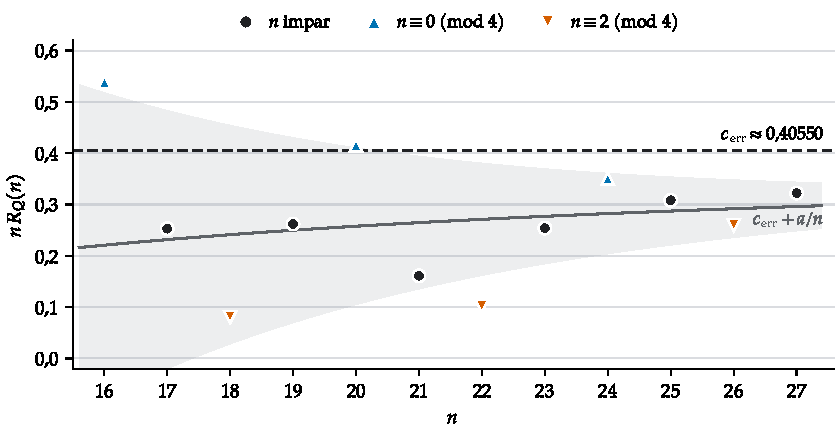
\includegraphics[width=.9\linewidth]{figuras/conteos.pdf}
\caption{Valores de $nR_Q(n)$ para $16\le n\le27$, obtenidos de los conteos exactos y del predictor
canónico (evidencia numérica). La línea discontinua marca el valor de $\cerr$ obtenido del continuo
y fijado antes del ajuste a estos doce tamaños. La curva gris
muestra la deriva ajustada $\cerr+a/n$, con $a\simeq-2{,}956$, y la banda sombreada tiene la amplitud
$Ae^{-\kappa(n-16)}$ de la oscilación de periodo cuatro (Apéndice~\ref{app:numquad}). Los tamaños
impares tienen oscilación ajustada cero. En los tamaños pares el modelo suma esa amplitud
si $n\equiv0\;(\mathrm{mod}\,4)$ y la resta si $n\equiv2\;(\mathrm{mod}\,4)$.}\label{fig:counts}
\end{figure}


\subsection{Reproducción del valor numérico}
El suplemento contiene las mallas finales, los programas de análisis, los valores en los nodos,
los intervalos y las huellas SHA256 de todos los archivos.
Con Python~3 y NumPy, la orden \texttt{python -B replica/reproducir\_valor.py replay}, ejecutada
desde \texttt{suplemento}, rehace el análisis en un directorio nuevo y debe dar $0{,}4055003786$ a
diez decimales. La guía del suplemento explica también cómo regenerar las mallas desde el principio.
La ejecución principal constó de 955 tareas y tardó 168,3 minutos con 16 procesos; la
complementaria, de 132 tareas y 30,1 minutos.

\subsection{Certificados por intervalos}
En \texttt{suplemento/certificados} están los programas que generan los intervalos del perfil, de
$S$, de $P_T$ y de $Q_2$ en el décimo nodo de la regla de Gauss--Legendre de veinte puntos, junto
con el núcleo bivariante con signo de ese nodo y una prueba rápida de las entradas. Cada
certificado registra la precisión empleada, sus entradas y el intervalo obtenido; la
Sección~\ref{sec:numcert} explica qué se certifica y hasta dónde.

\subsection{Predicciones registradas}
En las comprobaciones con tableros finitos, la predicción, los casos y la regla de comparación se
fijaron antes de evaluar, en un archivo con marca de tiempo y huella SHA256. El estudio del
cuadrado, por ejemplo, registró once predicciones: ocho en casos ciegos y tres en controles
conocidos.

\subsection{Estado de cada afirmación}\label{sec:claim-ledger}
La etiqueta \status{D} identifica los resultados demostrados.
Usamos \status{O} para una comprobación exacta por ordenador o un intervalo riguroso,
\status{N} para una estimación numérica y \status{D si C} para una cota demostrada bajo la
condición indicada. Los resultados marcados \status{D} se demuestran aquí dados los
enunciados importados de~\cite{pv,ef,pc,tc} (Sección~\ref{sec:importados}); esos cuatro trabajos
son preprints. La columna «Artículo» da la sección (un número) o el apéndice (una letra) de este
artículo. La columna «Supl.» remite a las tablas con letra del suplemento (sobre la prueba, las
torres y el cálculo numérico); esas letras no son los apéndices de este artículo.

La demostración del límite está asistida por ordenador en dos pasos. El cálculo racional
del Apéndice~\ref{app:pair} verifica los coeficientes de grado cuatro del par y del cuadrado.
Las cotas analíticas de sus restos son uniformes en la clase estacionaria. La
extrapolación de Richardson interviene al evaluar la fórmula para $\cerr$. El cotejo simbólico de
42 piezas constituye una comprobación independiente de la cancelación en el extremo.
{\small
\begin{longtable}{@{}L{.09\linewidth}L{.25\linewidth}L{.33\linewidth}L{.13\linewidth}L{.08\linewidth}@{}}
\toprule
Estado & Afirmación & Comprobación & Artículo & Supl.\\ \midrule
\endhead
\status{D} & Existencia del límite y fórmula exacta para $\cerr$~\eqref{eq:main} &
 Comparación de dos cortes del mismo tablero inicial &
 \ref{app:signed}--\ref{app:closing} & A B \\
\status{D} & Derivadas nulas en el extremo físico &
 Límite de las integrales truncadas y desarrollo de Taylor &
 \ref{app:closing} & A H \\
\status{D} & Identidad con signo y salidas a corte fijo &
 Historias detenidas, diferencia firmada y momentos &
 \ref{app:signed} & C D W \\
\status{D} & Resto de llegada en media, uniforme en el corte &
 Ley física, suma por tamaño y error de orden $b$ &
 \ref{app:arrival} & D \\
\status{D} & Densidad interior &
 Dieciséis términos y límite de Riemann a corte fijo &
 \ref{app:interior} & E Z \\
\status{D} & Torres en la frontera y cuadrado &
 Supervivencia y multiplicidad. Coeficiente del cuadrado por cálculo exacto \status{O} &
 \ref{app:boundary}, \ref{app:pair} & D G \\
\status{D} & Respuesta del par $J=-B_2+L_2$ &
 Ocho submedidas y reinserción de rango dos &
 \ref{app:weights}, \ref{app:transfer} & F X \\
\status{D} & Desarrollo de torres y estabilidad &
 Resto uniforme, menores y borrado con pesos &
 \ref{app:rook} & I K Y \\
\status{D} & Incremento restringido de la marginal &
 Punto estacionario, determinante y pesos físicos &
 \ref{app:pair} & B C L \\
\status{O} & Identidades racionales de la prueba asistida &
 Orden cuatro en siete variables para el par, dieciocho para el cuadrado &
 \ref{app:pair} & L D \\
\status{O} & Controles algebraicos &
 27 coeficientes de marginal y control del extremo transcrito &
 --- & M H \\
\status{N} & Estimación decimal y banda conservadora &
 Extrapolación de mallas y presupuesto empírico &
 \ref{sec:numeval} & P \\
\status{N} & Integral numérica de $\numerr_F/x^2$ &
 Cotejo con $F(0)+F'(0)-F(1)$ &
 \ref{sec:presupuesto} & P \\
\status{D si C} & Serie y cuadratura de $\numerr_6/x^2$ &
 Error $\le8{,}74\cdot10^{-10}$ bajo las tolerancias de muestreo &
 \ref{sec:presupuesto}, \ref{app:numquad} & P Q \\
\status{O} & Perfil físico y términos nodales explícitos &
 Intervalos exteriores y cobertura por fila &
 \ref{sec:numcert} & R \\
\status{O} & Integrales de frontera $S$ y $P_T$ &
 Cubatura certificada y recurrencia intervalar &
 \ref{sec:numcert} & R T \\
\status{O} & $Q_2$ completo en un nodo real &
 Encierros del núcleo y trazas con signo &
 \ref{sec:numcert} & T \\
\status{O} & Mayorantes globales &
 La anchura de la integral impide certificar el signo &
 \ref{sec:numcert} & R \\
\status{O} & Conteos $Q(n)$ hasta 27 &
 Valores enteros de las enumeraciones citadas &
 \ref{sec:ajuste-finito} & N \\
\status{N} & Residuos $nR_Q(n)$ en tamaños finitos &
 Evaluación del predictor, oscilación y deriva ajustadas &
 \ref{sec:conteos-exactos}, \ref{sec:ajuste-finito} & N \\
Abierto & Encierro fino de $\cerr$ &
 Errores nodales, integración del par y resto de malla &
 \ref{sec:numcert}, \ref{sec:discusion} & P R T \\
Alcance & Llegada puntual y vetos arbitrarios &
 Bastan las versiones restringidas &
 \ref{sec:discusion} & A B \\
\bottomrule
\end{longtable}
}

\section{Discusión y problemas abiertos}\label{sec:discusion}
La comparación de dos cortes da la expansión relativa
\(Q(n)/Q_{\rm pred}(n)=1+\cerr/n+o(1/n)\). La ecuación~\eqref{eq:main} determina \(\cerr\) mediante
el perfil y los tres términos de frontera. Quedan dos cuestiones distintas.

La primera es certificar el signo y las cifras de \(\cerr\). El intervalo global obtenido contiene
cero. Estrecharlo exige
controlar los valores nodales completos y la media con signo \(J\). Una vía sería demostrar un
resto uniforme para la cuadratura espacial de las dieciséis contribuciones físicas. Ese resto
tendría que controlar las exclusiones diagonales y los núcleos con resolvente, en particular la
contracción \(Q_2\). En la vía del continuo, un encierro que conserve la dependencia entre
contribuciones con signo tendría que mejorar el semiancho observado en el décimo nodo GL20.

La segunda concierne al resto del conteo. Después de restar \(\cerr/n\) a \(R_Q(n)\), queda un error
\(o(1/n)\). Se desconoce su orden y si en él persiste la oscilación de periodo cuatro que se
observa a tamaños pequeños. El control puntual de la llegada
y la estabilidad con vetos arbitrarios son estimaciones más fuertes que las usadas aquí.

\section*{Uso de herramientas de inteligencia artificial}
Se utilizaron herramientas de inteligencia artificial para organizar las fuentes, cotejar
versiones, programar y ejecutar los cálculos numéricos y por intervalos, asistir en el desarrollo
de las demostraciones, preparar la composición y la reestructuración editorial del texto, y
realizar revisiones adversariales de extractos textuales y de las demostraciones.

\appendix
\section{Identidad con signo y estimación de llegada}\label{app:signed}
Al revelar una reina, la ley uniforme pondera cada hijo por sus completaciones y la ley
adaptativa lo pondera por el predictor. Al comparar ambas a lo largo de una historia hay que
conservar la normalización de cada fila y el valor del predictor al detenerse.
Sea \(\mu\) la ley de la solución uniforme con el orden independiente de filas, y sean \(\nu\)
y \(\nu^\sharp\) las leyes adaptativas de \(L\) y \(L^\sharp\). Dada la fila \(i\), pongamos
\[
 \rho^\sharp(B,i)=\sum_{e\in i}\exp(L^\sharp(B+e)-L^\sharp(B)),\qquad
 A^\sharp=\sum_{t<\tau}\log\rho^\sharp(B_t,i_t).
\]
Aquí \(t\) cuenta los pasos de revelado en la suma y todos los hijos disponibles, incluidos los de salida,
intervienen en la normalización. Sea \(g^\sharp=\log Q-L^\sharp\). En la llegada conservemos
sólo las restricciones de pares de un cuadrado físico \(C\) sobre la misma máscara de torres.
Denotemos por \(\gamma_C\) el logaritmo de la probabilidad de evitación bajo torres menos el
cambio correspondiente en el predictor. Sean \(\Gamma=\sum_C\gamma_C\) y
\(g^\flat=g^\sharp-\Gamma\). Los factores del orden de filas son iguales en las dos historias.
Las demás probabilidades se telescopan, pues la ley uniforme asigna a cada prefijo una masa
proporcional a su número de completaciones. Al invertir en \(F_b\), donde dicho número es
positivo y la historia tiene masa positiva bajo ambas leyes, se obtiene la identidad exacta
\begin{equation}\label{eq:signed-history}
 e^{-g^\sharp(B_n)}\nu^\sharp(F_b)
 =\mathbb E_\mu[\exp\{-A^\sharp-\Gamma-g^\flat\};F_b].
\end{equation}
En adelante \(\mathbb E[X;E]=\mathbb E[X\mathbf1_E]\). Para estimar la identidad necesitamos
la consistencia por fila y la difusión en los tableros que entran en la normalización.
Precisamos esta última propiedad para el hijo físico, también cuando es el primero que sale.
\begin{lema}[Escalado después de una jugada]\label{lem:hijo-fisico}
Sea un padre regular de tamaño \(m\) cuyo punto físico \(p^{Q}\) es positivo en su soporte
binario, tiene márgenes de fila y columna uno, \(p^{Q}_{ic}\le C/m\) y brecha de incidencia
al menos \(\gamma>0\). Fijada una casilla legal \(e\), fórmese el menor de torres \(M_e\)
y prohíbase cualquier subconjunto de las demás casillas de las dos diagonales de \(e\).
Para \(m\) suficientemente grande, todas esas máscaras de tamaño \(m-1\) tienen escalado en
una misma clase de difusión y brecha, con constantes que sólo dependen de \(C,\gamma\).
En particular esto vale para el hijo completo \(M_e^{\rm fis}\) en la primera salida.
\end{lema}
\begin{proof}
Eliminamos una columna en cada fila retenida y hasta una casilla por cada diagonal.
La pérdida en cada fila es a lo sumo \(3C/m\), y lo mismo vale por columna. Sea \(R\) la
restricción de \(p^Q\) después de las eliminaciones y sea \(\mathcal W\) el lado con menos vértices
de un corte del grafo bipartito restante. En el padre, Rayleigh sobre el indicador centrado
da capacidad al menos \(\gamma |\mathcal W|/2\), pues \(|\mathcal W|\le m\).
Queda en \(R\) una capacidad de al menos \((\gamma/2-3C/m)|\mathcal W|\).
Oriente las aristas de filas a columnas. Los déficits de fila y los déficits de columna
con signo opuesto tienen suma cero y cada uno tiene módulo a lo sumo \(3C/m\).
Con \(\lambda=(3C/m)/(\gamma/2-3C/m)<1\), cada corte soporta la demanda neta
con capacidades simétricas \(\lambda R\). El criterio de flujo factible~\cite{gale} da una corrección
firmada
y una matriz bistocástica \((1-\lambda)R\le p'\le(1+\lambda)R\).
Su conductancia es al menos \((1-\lambda)(\gamma/2-3C/m)\). La desigualdad de Cheeger~\cite{lsok} da una
brecha
positiva uniforme para el laplaciano normalizado.

Falta transferir estas cotas de una tabla factible al escalado del soporte binario.
En tamaño \(k\), sea \(a\) bistocástica, positiva en el soporte, con \(a_{ic}\le C'/k\)
y brecha \(\gamma'\). El máximo de entropía en ese soporte es interior por la factibilidad
estricta. Sus ecuaciones dan el escalado \(D\) con \(\log(kD_{ic})=u_i-u_c\).
Por los márgenes, \(\sum a_{ic}\log(kD_{ic})=\sum D_{ic}\log(kD_{ic})\ge0\).
La parte positiva de la primera suma es a lo sumo \(\sum a_{ic}kD_{ic}\le C'k\).
Al restar una mediana de los potenciales e integrar los cortes de nivel se obtiene
\[
 \frac{\gamma'}2\sum_z|u_z|\le\sum_{ic}a_{ic}|u_i-u_c|\le2C'k .
\]
Fije \(T>8(C')^2/\gamma'\). Cada línea tiene al menos \(k/C'\) vecinos, y en todo el grafo
menos de \(k/(2C')\) vértices tienen \(|u_z|>T\). La ecuación de fila
\(1=e^{u_i}\sum_{c\sim i} e^{-u_c}/k\) da \(e^{u_i}\le2C'e^T\), y la de columna da
\(e^{-u_c}\le2C'e^T\). Las mismas ecuaciones con las cotas superiores dan cotas inferiores
recíprocas. Así \(d_-/k\le D_{ic}\le d_+/k\) en el soporte y
\(D\ge(d_-/C')a\) conserva una brecha positiva por Rayleigh.
Se aplica esto a \(p'\), con \(k=m-1\). Para la máscara del padre se aplica directamente a
\(p^Q\), también en la llegada larga regular. Los márgenes del predictor~\cite{pc} se obtienen
hasta la parada por el Corolario~4.12 y la clase interior de~\cite[def.~2.2 y §§4--5]{tc}.
Si la brecha se enuncia con pesos de respuesta, su comparabilidad con \(p^Q\) en la rama
de vacancias positivas da la hipótesis de Rayleigh.
\end{proof}

El coeficiente \(\coefT=\mathfrak F-1/12\) de (T) depende de las masas marcadas de fila y
columna \(s,t\) y del peso del cruce \(z\). Las expresiones integradas del
apéndice~\ref{app:rook} son holomorfas y acotadas en discos con radios de clase.
En \(s=0\) o \(t=0\) los términos visibles son independientes de \(z\).
Al derivar en \(z\), ambas caras se anulan. Si \(M_0\) acota \(\coefT\) en un
polidisco de radio \(r\) de clase en torno al punto de borrado en \(z\), Cauchy en
\(z\) acota \(|\partial_z\coefT|\) por \(2M_0/r\) en el disco reducido. Schwarz en las
masas \(s,t\) introduce los factores \(|s|/r,|t|/r\). Por tanto
\(\partial_z\coefT=st\,O(1)\) uniformemente, también al integrar en \(z\) a lo largo
del segmento de borrado. Las dos masas valen \(1/k\); en tamaño \(k\) esto da
\(O(k^{-3})\) para el cambio de \(\coefT/k\) por casilla vetada. Retirar una fila y una columna
cambia las masas en \(O(k^{-1})\) y el tamaño inverso en \(O(k^{-2})\), con coste
\(O(k^{-2})\) en \(\coefT/k\). Hay a lo sumo \(2m\) casillas vetadas. El lema proporciona
los mismos márgenes en todos los pasos. Sumando los cambios y usando el resto \(O(m^{-2})\)
de (T) en los dos extremos, obtenemos para todos los hijos del padre regular
\begin{equation}\label{eq:incremento-hijo-fisico}
 |g_T(M_e^{\rm fis})-g_T(M)|\le C/m^2,\qquad |g_T(M_e^{\rm fis})|\le C/(m-1).
\end{equation}


\paragraph{El signo de la salida.}
La cota \eqref{eq:incremento-hijo-fisico} y la consistencia del predictor ordinario dan
\(\lvert A^\sharp\rvert\le C_b/n\) hasta la parada, al sumar \(O(m^{-2})\) en \(m>j\).
En \(F_b\) la difusión da \(|\Gamma|\le C/j\). Pongamos \(U_0=A^\sharp+\Gamma\).
El Lema~\ref{lem:llegada-integrada} acota el coste de reemplazar \(e^{-g^\flat}\) por uno en
\eqref{eq:signed-history}, pues \(e^{-U_0}\le e^{C_b/n}\).
El resto de Taylor de \(e^{-U_0}\) es \(O_b(n^{-2})\).
La cota previa \(R_Q(n)=O(n^{-1})\) del Lema~\ref{lem:previa}
y (T) dan \(g^\sharp(B_n)=O(n^{-1})\), con el mismo orden de resto para su exponencial.
Por tanto, con \(\limsup_n|\epsilon_n(b)|\le C_\delta b\),
\[
 n g^\sharp(B_n)\nu^\sharp(F_b)
 =n\mathbb E_\mu[U_0;F_b]+n\{\mu(F_b^c)-\nu^\sharp(F_b^c)\}+\epsilon_n(b).
\]
El signo se obtiene de \(\nu^\sharp(F_b)-\mu(F_b)=\mu(F_b^c)-\nu^\sharp(F_b^c)\).

El cociente de probabilidades de hijo bajo \(\nu^\sharp\) y \(\nu\), dada la fila, es
\(e^{g_T(M_e^{\rm fis})}/\mathbb E_{\nu,i}e^{g_T(M_{e'}^{\rm fis})}\).
Todos los hijos del padre regular cumplen \(|g_T|\le C/(m-1)\), incluido el de primera
salida. El logaritmo del cociente está entre \(-2C/(m-1)\) y \(2C/(m-1)\), pues el
denominador promedia sobre todos los hijos. El producto detenido queda acotado por
\(\exp(2C\sum_{m=j+1}^n(m-1)^{-1})=\exp(O_{b,\delta}(1))\). Con \(X=Qe^{-L}\),
la densidad de \(\mu\) respecto de \(\nu\) es \(Xe^{A-R_Q(n)}\), donde \(A\) suma los
logaritmos de las normalizaciones de fila ordinarias. En el tramo macroscópico la probabilidad
de salida bajo \(\nu\) es exponencialmente pequeña por~\cite[cor.~4.12]{tc}, y el coste
ponderado por \(e^AX\) se acota por
\(C\exp(-c_\delta n+C_\delta n^{2/3}+O_\delta(n^{-1}))\).
Para cada banda diádica de la parada con suelo \(j\), de escala \(m\ge j/2\), el coste con
peso \(1+X\) es
\(C e^{-(c_*-2\beta)m}\), con \(c_*>2\beta\).
El Lema~\ref{lem:prescripcion-larga} acota la llegada larga en \(O(e^{-2j})\) con ese peso.
Al sobrevivir el tramo macroscópico se cumple \(|A|\le C_\delta/\lceil\delta n\rceil+C/j\).
El Lema~\ref{lem:positividad-llegada} da \(F_b^c\subset H_j^c\). La suma por bandas y la
cota macroscópica controlan \(\nu(H_j^c)\) y \(\mu(F_b^c)\) a orden exponencial.
El producto detenido da ese orden para \(\nu^\sharp(F_b^c)\). Retirar el indicador en la media
de \(A^\sharp\) cuesta entonces \(o_b(1)\) tras multiplicar por \(n\). Se sigue que
\begin{equation}\label{eq:signed-mean}
 \limsup_n\left|n g^\sharp(B_n)-n\mathbb E_\mu A^\sharp
                 -n\mathbb E_\mu[\Gamma;F_b]\right|\le C_\delta b .
\end{equation}
\section{Suma del resto en la llegada}\label{app:arrival}
Un solo cuadrado puede contribuir a la escala \(1/n\) que interesa en \eqref{eq:signed-mean}.
Al sustraer \(\Gamma\), cada soporte que sobrevive debe satisfacer las restricciones geométricas
de dos cuadrados. Ese coste adicional permite sumar los errores con una cota que decrece con \(b\).
Veámoslo primero en la llegada histórica corta \(H_j\), bajo \(\nu\). Para un conjunto
de casillas \(Y\), activamos sólo las restricciones diagonales soportadas en \(Y\), manteniendo
la máscara de torres completa. Llamemos \(e(Y)\) al logaritmo de la probabilidad de evitación
menos el cambio de predictor, y \(e_C(Y)\) a la misma expresión usando sólo los pares de \(C\).
El coeficiente de un soporte \(U\) es \(\sum_{Y\subseteq U}(-1)^{|U|-|Y|}e(Y)\).
Una casilla aislada se cancela al emparejar subconjuntos que difieren sólo en él. Si todos los
pares pertenecen a un cuadrado, el coeficiente se cancela con el de \(e_C\).
Si intervienen dos cuadrados distintos, ningún \(e_C\) contribuye: las casillas tendrían que
estar en los cuatro vértices de \(C\), cuyas únicas parejas diagonales son las dos de \(C\).
El resto suma por tanto los coeficientes originales que carecen de casillas aisladas y contienen
al menos dos cuadrados distintos. Lo sustraído tiene grado a lo sumo cuatro.

Sean \(v\) el número de casillas, \(h\) el total de etiquetas distintas de filas y columnas,
\(D\) el número de coordenadas libres y \(p\) el exponente del soporte. Prescribir las
\(h\) líneas da el factor \((j/n)^h\), junto con \(\delta^{-2v}\exp(C_Lv^2/j)\) en la
cota de prescripción. Para cada tipo, el número de posiciones es de orden \(n^D\).
Escribamos \(d_*=h-D\), \(q=p-D-1\). Dos cuadrados distintos imponen dos ecuaciones
lineales no proporcionales sobre las coordenadas de fila y columna. Así \(d_*\ge2\);
la cota del soporte da \(q\ge0\). El factor escalado es
\[
 n\,n^D j^{-p}(j/n)^h=(j/n)^{d_*-1}j^{-q}
 \le (b/\delta_*)\delta_*^{d_*-1}j^{-q}
 \qquad(0<b\le\delta_*).
\]
Extraemos \(b/\delta_*\) antes de sumar. Para \(v\le4\) el número de tipos tiene una cota
absoluta. Para los tipos no colineales el recuento ponderado usa \(d_*-1+q\ge(v-4)/3\).
De ahí que para \(5\le v\le N=\lceil4\log n/\log\rho\rceil\), fijado \(\rho\ge2\), la cota
tras sumar los tipos de ese tamaño sea
\[
 (b/\delta_*) C_L(C_1\delta^{-2})^v v^{d_{\rm pol}}\delta_*^{(v-4)/3}.
\]
Se elige \(\delta_*\) de manera que \(C_1\delta^{-2}\delta_*^{1/3}<1\).
En un tipo colineal \(v\ge3\) se tiene \(p=v+2,h=2v\), con a lo sumo \(4n\,n^v/v!\)
soportes. Resulta \(C(C_2\delta^{-2})^v v^2(j/n)^{v-2}\); se reduce \(\delta_*\)
una vez para sumar también esta cota. La sustitución de átomos hasta grado \(N\) cuesta
\(O(j^{-8})\) en valor, y la norma global acota la cola por \(O_\rho(n^{-2})\).
Ambos errores desaparecen tras escalar para cada \(b\) fijo. Así
\(\limsup_n n\mathbb E_\nu[|g^\flat|;H_j]\le C_\delta b\), con \(C_\delta\)
independiente de \(b\).

La cota obtenida controla una media de \(|g^\flat|\) bajo \(\nu\). En \eqref{eq:signed-history}
interviene además la exponencial bajo \(\mu\). El factor \(X\) de la densidad permite estimar
ambas con la misma cota, pues en la llegada se tiene
\[
 X\,|e^{-g^\flat}-1|=e^{g_T+\Gamma}|1-e^{g^\flat}|.
\]
En \(H_j\) la parte positiva del error diagonal tiene una cota de clase,
\(|g_T|+|\Gamma|\le C/j\) y \(|A-R_Q(n)|=O_{b,\delta}(1/n)\).
Se aplica \(|e^y-1|\le e^{y^+}|y|\) a la densidad \(Xe^{A-R_Q(n)}\).
En \(F_b\setminus H_j\) la probabilidad ponderada es \(O(e^{-2j})\).
Para \(0<X\le1\) vale \(X|\log X|\le1/e\); por encima de uno se usa
\(X|\log X|\le X(C_0+\beta j)\) en la clase exterior. El aporte de este suceso al lado
izquierdo de \eqref{eq:arrival-estimate} antes de escalar es \(O((1+j)e^{-2j})\).
Para obtener \eqref{eq:arrival-estimate} fijamos primero \(\delta\), los márgenes, \(\rho\) y
las constantes de clase, después \(\delta_*\) y por último el corte. El umbral de \(n\) puede
depender de \(b\). La constante \(C_\delta\) sirve para todos esos cortes, como exige la
comparación final de dos cortes en el apéndice~\ref{app:closing}.

\section{La media interior a corte positivo}\label{app:interior}
Para hallar la contribución interior a \eqref{eq:signed-mean} fijamos el corte \(b>0\).
Cuando quedan \(m>\lfloor bn\rfloor=j\) filas, escribimos \(x=m/n\).
La elección de una casilla modifica el predictor en orden \(1/m\) después de descontar
\(\log p_c\). Para identificar lo que queda en orden \(1/m^2\) empezamos en un padre regular,
antes de promediar sobre las historias.

\subsection{La inserción de una casilla}
Sean \(c\) la casilla elegida, \(\mathcal J=\familias(c)\) sus cuatro líneas, \(I\) las líneas retenidas,
\(F\) las casillas disponibles que tocan \(\mathcal J\), incluido \(c\), y \(E'\) las que sobreviven.
Para cada casilla \(i\), sea \(a_i\) el vector de incidencia de sus cuatro líneas.
Con \(h_f=1-\sum_{i\in f}p_i\) en las diagonales, pongamos
\begin{align*}
 S_0&=\sum_i p_i a_i a_i^{\mathsf T}+\operatorname{diag}(0_R,0_C,h_D,h_A),
 & R&=S_0^+,\\
 t_{ic}&=a_i^{\mathsf T}Ra_c,
 & w_i&=6p_i+f_i,\qquad f_i=\sum_{\{u,v\}\subset \familias(i)}R_{uv}.
\end{align*}
Las sumas sobre pares no ordenados usan dos líneas distintas. En \(E'\), escribamos
\(y_i=p_i^{(c)}-p_i\), donde \(p^{(c)}\) es el punto estacionario del hijo, y
\(q_i=y_i/p_i+t_{ic}\). La respuesta del hijo da \(q_i=O_b(m^{-2})\).
El potencial completo del prefactor es
\(V=\ell+\tfrac12\log\det S_{0,\rm gf}+3\sum_i p_i^2\). En los soportes conexos de
la clase, \(L=H+\ell+\tfrac12\log(2\pi)\) y \(\ell\) incluye el cofactor del predictor.
En \(\det S_{0,\rm gf}\) se usa el mismo calibre en padre e hijo.
La corrección lineal y su centrado se leen en
\[
 \delta_c^0=-w_c+\sum_i p_i t_{ic}w_i,\qquad
 \sum_{c\in r}p_ca_c=S_0 e_r,\qquad a_i^{\mathsf T}RS_0 e_r=(a_i)_r .
\]
La última igualdad usa que \(a_i\) es ortogonal al modo nulo fila--columna.
Por tanto \(\sum_{c\in r}p_c\delta_c^0=0\) para cada fila \(r\).

La consistencia por inserción~\cite[Teorema 7.1 y Corolario 7.2]{pc} da
\(L(B+c)-L(B)=\log[p_c(1+\delta_c)]+r_c^{\rm PC}\), con
\(\sum_{c\in r}p_c\delta_c=0\), \(\delta_c=O_b(m^{-1})\) y \(r_c^{\rm PC}=O_b(m^{-2})\).
Al desarrollar la exponencial en esos pesos de masa uno y después el logaritmo se obtiene
\(\log\rho(B,r)=\sum_{c\in r}p_c r_c^{\rm PC}+O_b(m^{-3})\).
El cambio de pesos en el término lineal cuesta \(O_b(m^{-3})\).

\paragraph{Qué términos deja el cambio de soporte.}
Descompongamos \(S_0\) en bloques \(B_0,C_0,C_0^{\mathsf T},D_0\) según \(I,\mathcal J\).
Sea \(U_0=\sum_{i\in F}p_i a_{i,I}a_{i,I}^{\mathsf T}\),
\(\mathcal M=B_0-U_0\), \(d_0=C_0\mathbf1\), \(\beta=Ra_c\),
\(z=\beta_I\), \(t=\beta_{\mathcal J}-\mathbf1\) y \(r=d_0+\mathcal M z=-C_0t-U_0z\).
El mínimo de la energía cuadrática del hijo es \(Q_*=d_0^{\mathsf T}\mathcal M^+d_0\).
Al insertar \(d_0=r-\mathcal Mz\) y usar \(S_0\beta=a_c\) se obtiene
\[
 Q_*=a_c^{\mathsf T}Ra_c-4+12p_c+E_Q,\qquad
 E_Q=z^{\mathsf T}U_0z-t^{\mathsf T}D_0t+r^{\mathsf T}\mathcal M^+r .
\]
En efecto \(D_0=(1-p_c)I+p_c\mathbf1\mathbf1^{\mathsf T}\) y
\(\mathbf1^{\mathsf T}D_0\mathbf1=4+12p_c\). Se tiene \(r=O_b(m^{-2})\) por entrada
y \(r^{\mathsf T}\mathcal M^+r=O_b(m^{-3})\) por la brecha y el número \(O_b(m)\) de líneas.

Sea \(\gamma_f=h_f^{(c)}-h_f\) el cambio de vacancia en una diagonal retenida.
Taylor de la entropía del apéndice~\ref{app:predictor}, con los pesos del hijo, da
\begin{align*}
 \Delta H-\log p_c&=\tfrac32\sum_{F\setminus\{c\}}p_i^2-\tfrac12 Q_*+A_3+O_b(m^{-3}),\\
 A_3&=\sum_{F\setminus\{c\}}p_i^3+\tfrac16\sum_{E'}p_i(y_i/p_i)^3
 +\tfrac32\sum_{E'}\frac{y_i^2}{1-p_i}+\tfrac16\sum_{f\in I_D}\gamma_f^3/h_f^2 .
\end{align*}
Aquí \(I_D\) recorre ambas familias diagonales retenidas. Los términos cuárticos cuestan
\(O_b(m^{-3})\) por \(\sum p_i=m\), \(p_i=O_b(m^{-1})\) y
\(|y_i/p_i|+|\gamma_f/h_f|=O_b(m^{-1})\). La ortogonalidad en el mínimo deja un error
cuadrático en las correcciones relativas \(O_b(m^{-2})\) a la respuesta lineal.

Para el cofactor escribamos \(\Pi_m=vv^{\mathsf T}/(2m)\), donde \(v\) vale \(1,-1,0,0\)
en las cuatro familias. Sean \(H_*=(R+\Pi_m)_{II}\), \(C_{\mathcal J}=D_0+(\Pi_m)_{\mathcal J\mathcal J}\),
\(V_{\mathcal J}=C_0+(\Pi_m)_{I\mathcal J}\) y \(\Pi'=v_Iv_I^{\mathsf T}/[2(m-1)]\).
En \(I\), \(S_*\) tiene entrada \(-p_i\) en cada par ordenado de líneas distintas
de \(i\in F\setminus\{c\}\). En forma análoga \(Y\) tiene entrada \(y_i\) en los pares de
\(i\in E'\). Sus restantes entradas son cero. El complemento de Schur da
\begin{align*}
 D_*&=S_*+Y+\Pi'-(\Pi_m)_{II}+V_{\mathcal J} C_{\mathcal J}^{-1}V_{\mathcal J}^{\mathsf T},\\
 Q_c&=\tfrac{m^2}4\{\operatorname{tr}[(H_*D_*)^2]-\operatorname{tr}(S_*^2)\},\\
 E_R&=\operatorname{tr}[(C_{\mathcal J}-I)(H_{\mathcal J}-I)],\qquad H_{\mathcal J}=(R+\Pi_m)_{\mathcal
 J\mathcal J}.
\end{align*}
Para la normalización del calibre sean \(S'_0\) la matriz del hijo y
\(\Delta_0=S'_0-(S_0)_{II}\). Su contribución se obtiene de
\[
 E_g=\log[m/(m-1)]-\log\det C_{\mathcal J}
   +\operatorname{tr}[(\Pi_m)_{II}\Delta_0]
   +\operatorname{tr}[H_*(\Pi'-(\Pi_m)_{II})].
\]
Como \(v_{\mathcal J}\perp\mathbf1\), \(\det C_{\mathcal J}=(1+3p_c)(1-p_c)^2(1-p_c+1/m)\).
Los logaritmos dan \(m^{-2}-p_c/m+6p_c^2+O_b(m^{-3})\). Las dos trazas valen
\(-(1-p_c)/m\) y \((m-1)/m^2+v_{\mathcal J}^{\mathsf T}R_{\mathcal J\mathcal J}v_{\mathcal J}/[2m(m-1)]\),
 respectivamente,
por \(S_0v=Rv=0\). Como \(R_{\mathcal J\mathcal J}=I+O_b(m^{-1})\), queda \(E_g=m^{-2}+6p_c^2+O_b(m^{-3})\).
El cubo del logaritmo del determinante deja \(C^{(3)}=-\operatorname{tr}(S_*^3)/6\).
En efecto, las filas de \(S_*\) tienen suma absoluta \(O_b(m^{-1})\);
las entradas de \(D_*-S_*\) son \(O_b(m^{-2})\) y las de \(H_*-I\) son \(O_b(m^{-1})\).
En la traza cúbica, un factor de \(H_*D_*-S_*\) cuesta así \(O_b(m^{-3})\) en total.
Las potencias de orden cuatro o superior tienen la misma cota por la norma de filas.
La traza pura \(\operatorname{tr}(S_*^2)/4\) aporta
\(3\sum_{F\setminus\{c\}}p_i^2/2\), pues hay seis pares ordenados en cada casilla retirada.

En la parte lineal de Schur, sea \(f_i^I\) la restricción de \(f_i\) a pares retenidos.
Las cuatro entradas diagonales de \(S_0R=I-\Pi_m\) sobre \(\mathcal J\) dan
\[
 \sum_{i\in F}p_i(f_i-f_i^I)
 =-\operatorname{tr}[(R-I)_{\mathcal J\mathcal J}]-1/m-p_cf_c .
\]
Al juntar la traza lineal, \(-Q_*/2\), las dos copias de
\(3\sum_{F\setminus\{c\}}p_i^2/2\) y \(-3\Delta\sum p_i^2\), los términos con \(w_i\)
son \(\sum_F p_iw_i-w_c-\sum_{E'}y_iw_i\) y queda \(p_cf_c-3p_c^2\).
Restar \(\delta_c^0\) convierte las dos sumas en las de la última línea de la fórmula
\begin{align*}
 L(B+c)-L(B)-\log p_c-\delta_c^0
   &=\Delta_c V+P_c+O_b(m^{-3}),\\
 P_c&=-E_g/2+Q_c/m^2+C^{(3)}+A_3-3\sum_{E'}y_i^2\\
 &\quad-3p_c^2+p_cf_c-(E_Q+E_R)/2\\
 &\quad+\sum_F p_i(1-t_{ic})w_i-\sum_{E'}p_iq_iw_i .
\end{align*}


Puesto que \(\delta_c-\delta_c^0=O_b(m^{-2})\), desarrollar \(\log(1+\delta_c)\) da
\[
 r_c^{\rm PC}=\Delta_c V+P_c+\tfrac12(\delta_c^0)^2
                   +(\delta_c^0-\delta_c)+O_b(m^{-3}).
\]
El último paréntesis desaparece exactamente al promediar en la fila. Los errores cúbicos
acumulados cuestan \(O_b(n\sum_{m>j}m^{-3})=O_b(n^{-1})\). La tabla identifica qué
parte de \(m^2[P_c+(\delta_c^0)^2/2]\) origina cada contribución al perfil.
\begin{center}\small
\begin{tabular}{ll}
\toprule
Término de inserción a escala \(m^2\) & Contribución al perfil\\ \midrule
\(-m^2 E_g/2\)& \(G_{\rm cof}\)\\
\(m^2 A_3\)&\(f2E+f2z+f2F\)\\
\(m^2 C^{(3)}\)&\(f2F+C_{3,\rm cuad}\)\\
\(-m^2(E_Q+E_R)/2\)&\(f3F+f3c\)\\
\(m^2(-3p_c^2+p_c f_c)\)&\(f4=f4_{\rm expl}+f4_{L0}\)\\
\(m^2\sum_F p_i(1-t_{ic})w_i\)&\(f5c+f5F\)\\
\(-m^2\sum_{E'}p_iq_iw_i\)&\(f6\)\\
\(m^2(\delta_c^0)^2/2\)&\(f7\)\\
primera parte de \(Q_c\)&\(Q_1+\Delta_1\)\\
segunda parte de \(Q_c\), con \(-3m^2\sum_{E'}y_i^2\)&\(Q_2+\Delta_2\)\\
\bottomrule
\end{tabular}
\end{center}
\subsection{Las dieciséis contracciones del perfil}\label{sec:contracciones}
Denotamos por \(\langle g\rangle_i=\int_{[0,1]^2}\nu_1(i)g(i)\,di\) la media de área y
por \(\langle\cdot\rangle_c\) la misma media en el centro. En la fibra \(\lambda\)
de \(c\), \(d\omega_\lambda(i)=\eta_\lambda\nu_1(i)\,dy\), con \(y\) la coordenada libre
de fila o columna y, en las diagonales, la coordenada de fila. Para una función \(g\),
\(\int_F g=\sum_{\lambda\in \familias(c)}\int_{i\in\lambda}g(i,\lambda)\,d\omega_\lambda(i)\).
La medida \(d\rho\) de una línea libre es \(dy\) en
cada familia axial y \(U_f\,dy/(2x)\) en cada hoja de una familia diagonal.
El factor \(1/2\) ya realiza la media en la hoja de esa línea libre. Los demás índices
enteros libres aportan sus propias clases de paridad, según su parametrización. En una fibra
axial el desplazamiento tiene dos paridades de igual peso. En una diagonal el desplazamiento
mantiene el color. Un cruce diagonal--antidiagonal sólo existe en hojas compatibles.

\paragraph{Qué disponibilidad lleva una intersección.}
En una configuración fijamos las líneas de sus casillas marcadas y las líneas que se integran
con \(d\rho\). Sea \(\mathcal A\) ese conjunto. A cada otra línea \(\ell\) de una configuración
finita se le asigna una variable de Bernoulli independiente \(X_\ell\) de media \(U_\ell\).
En \(\mathcal A\) se pone \(X_\ell=1\). Sean \(\familias(z)\) las cuatro líneas de \(z\),
\(Y_z=\prod_{\ell\in \familias(z)}X_\ell\) y \(\pesodirecto(z)=W(z)Y_z\). Un cruce ausente da
 \(\pesodirecto=0\).
Así el peso de varias casillas directas \(Z\) se obtiene de
\[
 \psi(Z)=\mathbb E\prod_{z\in Z}Y_z
 =\prod_{\ell\in(\bigcup_{z\in Z}\familias(z))\setminus\mathcal A}U_\ell .
\]
El mismo indicador se usa en todo el monomio. Para el núcleo \(L_0\) y la corrección
\(\theta\) de la sección~\ref{sec:profile-data}, la respuesta de dos líneas es
\[
 E(a,b)=
 \begin{cases}
 (L_0)_{aa}+\theta_a,&a=b,\\
 (L_0)_{ab}-\pesodirecto(a\cap b),&a\ne b .
 \end{cases}
\]
Una casilla marcada aporta \(\pesodirecto(i)=W(i)\). Abreviamos
\(z_f=\sum_{j\in \familias(c)}E(f,j)\), \(T_i=\sum_{a\in \familias(i)}z_a\),
\(t_j=z_j\) para \(j\in \familias(c)\), y \(w(i)=\sum_{\{a,b\}\subset \familias(i)}(L_0)_{ab}\).
En particular \(t_j\) y \(w(i)\) en una casilla marcada son deterministas.
Para \(i\) que sólo comparte \(\lambda\) con \(c\), sea
\(\sigma_i=\sum_{a\in \familias(i)\setminus\{\lambda\}}z_a\).

\paragraph{Cubo, energía y corrección de fila.}
Las contribuciones del cubo de la acción son
\begin{align*}
 f2E&=\left\langle-\tfrac16\mathbb E T_i^3+\tfrac32 W(i)\mathbb E T_i^2\right\rangle_{i,c},\\
 f2z&=-\tfrac16\left\langle\int_{D\cup A}(u_f/U_f)\,\mathbb E z_f^3\,d\rho(f)\right\rangle_c,\\
 f2F&=\left\langle\int_F W(i)^2\right\rangle_c .
\end{align*}
En \(f2E\) se marcan \(i,c\), independientes en área. En \(f2z\) se marcan \(c,f\).
Para verificar los momentos en estos dos casos, sumemos sobre los pares de líneas que definen
\(T_i\) o \(z_f\). Sean \(A_1,A_2,A_3\) las sumas respectivas de \(L_0-K\),
\(K(W_{ab}-K)\) y \(-K(W_{ab}-K)(W_{ab}-2K)\), con \(W_{ab}=W(a\cap b)\) o cero.
En posición general las transversales de cruces distintos son distintas. El segundo momento es
\(A_1^2+A_2\) y el tercero \(A_1^3+3A_1A_2+A_3\), por los momentos centrados de cada Bernoulli.
El factor \(u_f/U_f\) es la vacancia del punto estacionario en la línea retenida.

Con \(I_2=\langle W(c)^2\rangle_c\) y \(\Xi=\langle W(c)w(c)\rangle_c\), se obtiene
\[
 G_{\rm cof}=-\tfrac12-3I_2,\qquad f4=-9I_2+\Xi,\qquad f5c=-3\Xi .
\]
En efecto \(mf_c\) tiende al factor \(w(c)-6W(c)\), y \(1-t_{cc}=-3+O_b(m^{-1})\).
Las otras contracciones del centro y de la fibra son
\begin{align*}
 f3F&=-\tfrac12\left\langle\int_F\mathbb E\sigma_i^2\right\rangle_c,\\
 f3c&=\tfrac12\left\langle\sum_{j\in \familias(c)}t_j^2
 -\sum_{j,h\in \familias(c)}[W(c)(1-\delta_{jh})+\Pi_{jh}]
                         [E(h,j)+\Pi_{hj}]\right\rangle_c,\\
 f5F&=-\left\langle\int_F w(i)\mathbb E T_i\right\rangle_c,\\
 f7&=\tfrac12\left\langle\left[-w(c)+\int_F w(i)
                  +\left\langle w(i)\mathbb E T_i\right\rangle_i\right]^2\right\rangle_c .
\end{align*}
Aquí \(\Pi_{jh}=v_jv_h/2\) es el núcleo del perfil. El primer sumando de \(f3c\)
procede de \(t^{\mathsf T}D_0t\) y el segundo de \(E_R\).
En \(f3F\), \(i,c\) están marcadas en la misma fibra. Sean \(Z\) los cruces existentes
\(a\cap j\), con \(a\in \familias(i)\setminus\{\lambda\}\) y \(j\in \familias(c)\setminus\{\lambda\}\),
de familias distintas. En posición general son casillas distintas. Escribiendo
\(\psi_z=\psi(\{z\})\), el signo negativo de cada parte directa desaparece en la covarianza,
\begin{align*}
 \mathbb E\sigma_i^2={}&(\mathbb E\sigma_i)^2+\sum_{z\in Z}W(z)^2\psi_z(1-\psi_z)\\
 &+\sum_{\substack{z,z'\in Z\\z\ne z'}}W(z)W(z')
       [\psi(\{z,z'\})-\psi_z\psi_{z'}].
\end{align*}
Por ejemplo, en coordenadas relativas a \(c=(0,0)\), si \(i=(0,s)\), los cruces
\((s,s)\) y \((s,0)\) comparten la fila \(s\). Cuando existen dentro del tablero, su peso
conjunto es \(\psi_z\psi_{z'}/U_R\). En \(f7\) las dos copias de la suma tienen índices
libres distintos. Tras fijar \(c\), sus coincidencias accidentales tienen medida nula.
Así se cuadran las integrales de la respuesta centrada antes de promediar en \(c\).

\paragraph{Triángulos de líneas en la traza cúbica.}
Tres líneas del producto \(S_*^3\) concurren en una casilla borrada o cortan tres casillas
distintas que completan un cuadrado con \(c\). En el primer caso sus seis órdenes cancelan
el divisor \(6\), y el resultado es otra copia de \(f2F\).
Para el segundo, tomemos la base \(((1,0),(0,1))\) o \(((1,1),(1,-1))\) y multipliquemos
cada vector por un signo independiente, obteniendo \(v,w\). Sean
\(Z=\{c,c+hv,c+hw,c+h(v+w)\}\), \(h>0\), y \(n_{RC}\) el número de líneas axiales de \(Z\).
Las tres coordenadas libres son las de \(c\) y el paso primitivo \(h\). El resultado es
\[
 C_{3,\rm cuad}=\sum_{v,w}\int_{\{(c,h):\,Z\subset[0,1]^2\}}
  x^{n_{RC}-3}\prod_{z\in Z}W(z)
  \prod_{\ell\in(\bigcup_{z\in Z}\familias(z))\cap(D\cup A)}U_\ell\,dc\,dh .
\]
Los cuatro factores \(W\) incluyen el peso del centro. En la cuadratura el lado cero
lleva la mitad del valor límite del integrando. En la integral tiene medida cero.

\input{partes/prueba_respuesta}
\input{partes/reordenacion_f6}
\input{partes/prueba_trazas_interior}

\subsection{Límite uniforme de las medias y suma sobre los niveles}
La regularidad antes de la parada da \(p_i\le C_b/m\), una vacancia diagonal
minorada y una brecha de filas y columnas~\cite[\S7]{pc}.
En consecuencia \(c_b I\le S_0+\Pi_m\le 4I\) para algún \(c_b>0\).
Para ver la cota inferior, la forma cuadrática es la suma de
\(\sum_i p_i(a_i^{\mathsf T}y)^2\) y \(\sum_f h_f y_f^2\), más la proyección de calibre.
El segundo término controla las componentes diagonales y la brecha controla las axiales
ortogonales al calibre. La cota superior sigue de la diagonal unidad de \(S_0\), de que su
masa fuera de la diagonal por fila es a lo sumo tres y de que la proyección actúa en su núcleo.

Sea \(A_m=S_0+\Pi_m-I\), \(M=(I+A_m)^{-1}=R+\Pi_m\) y \(r_b=1-c_b/4<1\).
El polinomio \(P_N=\tfrac14\sum_{h=0}^N[I-(I+A_m)/4]^h\) satisface
\(\|M-P_N\|_{\rm op}\le r_b^{N+1}/c_b\). Para controlar una entrada multiplicada
por \(m\) usamos \(M=I-A_m+A_mMA_m\). La suma absoluta de una fila de \(A_m\) es
a lo sumo cuatro y su máximo es \(O_b(m^{-1})\), luego
\(\|A_me_u\|_2=O_b(m^{-1/2})\) para todo \(u\). Así
\[
 \sup_{u,v}m\,|[A_m(M-P_N)A_m]_{uv}|\le C_b r_b^{N+1}.
\]
Esto acota el error en cada entrada de \(m(R-I)\) al sustituir \(M\) por \(P_N\)
en la identidad anterior. Las entradas originales y sus truncaciones están acotadas.

A \(N\) fijo, las potencias de \(S_0-I\) son sumas sobre sucesiones de líneas adyacentes.
Las inserciones de \(\Pi_m\) se simplifican usando \((S_0-I)\Pi_m=-\Pi_m\).
Un producto de recorridos es una suma finita de tipos de incidencia. Si dos etiquetas afines
son idénticas en un tipo, se cuenta la línea una vez. Una coincidencia adicional impone
una ecuación no constante y deja \(O_{b,N}(n^{d-1})\) posiciones entre las \(O(n^d)\)
de un tipo con \(d\) parámetros. En la diagonal, la ida y vuelta de longitud dos fuerza
la misma casilla en ambos pasos. Su contribución es \(3m\sum_{i\in u}p_i^2\), pues hay tres
elecciones de la otra línea. Su exceso sobre el producto de las medias da precisamente
\(\theta_u=3\eta_u s_u-\int K_{uv}^2\,d\rho(v)\). Los cruces entre diagonales se
cuentan en las clases de paridad de la sección~\ref{sec:contracciones}.

A cada tipo fijo se aplica el seguimiento de líneas hasta el corte auxiliar \(b/4\)
de~\cite[\S4]{tc}. A tolerancia fija \(\eta>0\), fuera de una excepción de probabilidad
exponencial, \(mp_i=W(i)(1+O_b(\eta+m^{-1}))\) en los sitios vivos y
\(h_f=u_f/U_f+O_b(\eta+m^{-1})\). Para un número fijo de marcas el riesgo en un paso es
la suma de sus riesgos individuales salvo \(O_{b,N}(n^{-2})\) por dobles ocupaciones.
Al multiplicar estas supervivencias hasta el nivel \(m\), una marca axial aporta \(x\)
y una diagonal aporta \(U_f(x)\), pues \(\partial_x\log U_f=(1-u_f)/U_f\).
La aproximación es uniforme en las marcas y en \(j\le m\le n\). Se toma primero \(n\to\infty\)
y luego \(\eta\downarrow0\). Las sumas normalizadas de cada clase son sumas de Riemann
sobre politopos fijos. Los factores del perfil son continuos en \(x\) con módulo común en
\([b,1]\) en cada pieza. Por tanto los truncados convergen uniformemente en los niveles
a integrales continuas de los recorridos.

Para aplicar el mismo argumento a \(mV\), sea \(\kappa_i=a_i^{\mathsf T}Ra_i-4\).
La expansión del prefactor~\cite[\S7]{pc} da, con la última suma sobre todas las líneas,
\[
 V=-14\sum_i p_i^3-\tfrac32\sum_i p_i^2\kappa_i
       +\tfrac94\sum_u\left(\sum_{i\in u}p_i^2\right)^2+O_b(m^{-2}).
\]
Las doce entradas fuera de la diagonal en \(m\kappa_i\) aportan \(-12W(i)\) en la
casilla marcada. Combinadas con \(-14\) dan \(4\langle W^2\rangle_i\).
Las partes largas y la diagonal corregida dan los sumandos con \(L_0,\theta\) de
la sección~\ref{sec:profile-data}. El cuadrado de la suma de fibra da su último término.

En las contracciones, el centro tiene masa uno, el exterior masa a lo sumo uno y las
cuatro fibras masa a lo sumo cuatro. La medida de las líneas libres tiene masa \(\le6/b\).
Los pasos de cuadrados tienen masa total \(\le8/b\). Al desarrollar la diferencia de productos,
la cota de cada entrada se multiplica sólo por masas y factores acotados para \(b\) fijo.
Así la cola del grado \(N\) es \(\le C_b r_b^{N+1}\), uniforme en el nivel tanto para la media
física como para su integral límite. El resto de la inserción en la escala \(m^2\) es
\(O_b(m^{-1})\). Tomar primero \(n\to\infty\) y después \(N\to\infty\) da
\begin{align*}
 \sup_{j<m\le n}\Big|
 \mathbb E_\nu\!\left[m^2\sum_{c\in i_m}p_c
       \big(P_c+(\delta_c^0)^2/2\big);H_j\right]-d(m/n)\Big|&\longrightarrow0,\\
 \sup_{j\le m\le n}\left|\mathbb E_\nu[mV(B_m);H_j]-\mathcal V(m/n)\right|
  &\longrightarrow0 .
\end{align*}
Aquí \(i_m\) es la fila revelada y \(H_j\) la llegada regular corta. Para promediar la fila
se usa primero el indicador de supervivencia anterior a su elección. Dado el padre, la fila
es uniforme y la media se convierte en \(m^{-1}\sum_c p_c(\cdot)\).
Cambiar ese indicador por \(\mathbf1_{H_j}\) en los observables acotados cuesta
\(O_b(\nu(H_j^c))\). La segunda fórmula usa todas las familias en el potencial.
Este argumento identifica una media sobre padres y da continuidad del límite en \([b,1]\).
La evaluación decimal de esas integrales por mallas requiere además una cota de su error espacial.

\paragraph{Los extremos y el cambio de ley.}
El error uniforme \(\epsilon_n(b)\) de la primera media contribuye a lo sumo
\(\epsilon_n(b)n\sum_{m>j}m^{-2}=o_b(1)\). El término de \(P_c+(\delta_c^0)^2/2\)
da por tanto \(\int_b^1d(x)x^{-2}\,dx\). Para \(\Delta_cV\), la probabilidad de un hijo
dada la fila bajo \(\nu\) es \(p_c(1+O_b(m^{-1}))\), y \(|\Delta_cV|\le C_bm^{-2}\).
La sustitución en la media cuesta \(O_b(m^{-3})\). Los incrementos centrados hasta la parada
forman una martingala de segundo momento \(O_b(\sum_{m>j}m^{-4})\).
Si \(M_\tau\) es su suma detenida, las diferencias son ortogonales en \(L^2(\nu)\).
Así \(n|\mathbb E_\nu[M_\tau;H_j]|\le n(\mathbb E_\nu M_\tau^2)^{1/2}\nu(H_j)^{1/2}\).
Como \(\sum_{m>j}m^{-4}=O(j^{-3})\), el coste a escala \(n\) es \(O_b(n^{-1/2})\).
En cada historia de \(H_j\) los incrementos realizados suman \(V(B_j)-V(B_n)\).
La segunda media uniforme da \(\mathcal V(b)/b-\mathcal V(1)\).

Hasta la parada, \(n|A|\le C_b\) para el predictor ordinario. Por el Lema~\ref{lem:previa},
\(n|R_Q(n)|\) también está acotado. En \(H_j\) ponemos
\(s=A-R_Q(n)+g_T+\Gamma\). Allí \(|s|=O_b(n^{-1})\) y la densidad inversa de historias
es \(e^{-s-g^\flat}\). Por \eqref{eq:arrival-estimate},
\[
 \int_{H_j}|d\mu-d\nu|
 \le\mathbb E_\mu[|1-e^{-s}|+e^{-s}|1-e^{-g^\flat}|;H_j]=O_b(n^{-1}) .
\]
Con las estimaciones de salida del apéndice~\ref{app:signed} se sigue que
\(n\mathbb E_\mu A=n\mathbb E_\nu[A;H_j]+o_b(1)\).
Para las torres pongamos \(u_e=g_T(M_e^{\rm fis})-g_T(M)\).
La máscara \(M_e^{\rm fis}\) se obtiene del menor simple \(M_e\) aplicando los dos vetos
diagonales del hijo. El cambio es \(O_b(m^{-2})\), incluido el paso que entra en la salida.
Así \(\log\rho^\sharp-\log\rho=\log\mathbb E_{\nu,i}e^{u_e}
 =\mathbb E_{\nu,i}u_e+O_b(m^{-4})\).
La densidad detenida y las cotas ponderadas de salida dan
\(D(\mu^\tau\Vert\nu^\tau)=\mathbb E_\mu[A+\log X]-R_Q(n)=O_b(1)\).
Sean \(d_m\) las entropías condicionales de las dos leyes de hijo dada la fila,
iguales a cero después de la parada. Las filas tienen la misma ley uniforme.
La descomposición de la entropía relativa en sus incrementos condicionales da
\(\sum_m\mathbb E_\mu d_m=D(\mu^\tau\Vert\nu^\tau)\). La desigualdad de
Pinsker~\cite{ct} acota la diferencia de las dos medias de \(u_e\) por \(2C_bm^{-2}\sqrt{d_m/2}\).
Por Jensen y Cauchy--Schwarz, la suma de estas diferencias a escala \(n\) cuesta
\(O_b(n(\sum_{m>j}m^{-4})^{1/2}D(\mu^\tau\Vert\nu^\tau)^{1/2})=O_b(n^{-1/2})\).
Los incrementos realizados de torres se telescopan y añaden
\((F(b)-1/12)/b-(F(1)-1/12)\) a los extremos anteriores. En conclusión, a cada corte fijo,
\[
 \lim_{n\to\infty} n\mathbb E_\mu A^\sharp
 =\int_b^1\frac{d(x)}{x^2}\,dx+\frac{G(b)}b-G(1)
 =\int_b^1\frac{\numerr(x)}{x^2}\,dx .
\]


\section{Las tres medias de frontera}\label{app:boundary}
En \(\Gamma\) se ha aislado cada cuadrado, pero sus dos pares diagonales pueden estar disponibles
a la vez. Para guardar el signo y contar una sola vez su interacción, empezamos por la
corrección de un par y después reunimos los dos pares en el cuadrado. Aquí \(p_e\) designa
la ocupación estacionaria de \emph{torres} en la máscara binaria.
Para un par diagonal disponible \(P=\{e,f\}\), sea \(\pi^{\rm ex}_P\) su probabilidad conjunta en
una colocación uniforme de torres. Sea \(\pi^T_P=\exp[L_T(M_P)-L_T(M)]\), donde \(M_P\) elimina sus
cuatro extremos de fila y columna. Con \(\mathsf G(e,f)\) la respuesta cruzada del punto estacionario
de torres y \(\chi_e\) su corrección relativa de una casilla, definimos
\[
 \pi_{1,P}=p_ep_f(1-\mathsf G(e,f)+\chi_e+\chi_f),\qquad
 X_P=p_ep_f(p_e+p_f)\mathsf G(e,f).
\]
Para un par solo la corrección del cuadrado es
\(\log(1-\pi^{\rm ex}_P)-\log(1-\pi_{1,P})-X_P+O(j^{-5})\).
Las probabilidades son \(O(j^{-2})\) y su diferencia es \(O(j^{-4})\); al integrar la derivada
logarítmica el error de linealización es \(O(j^{-6})\). El cuadrado completo da las correcciones
de sus dos pares y un término adicional \(-3\prod_{s\in\square}p_s+O(j^{-5})\).
Hay a lo sumo \(j^2(j-1)\) pares, pues cada casilla tiene a lo sumo \(2(j-1)\) vecinas y cada
par tiene dos extremos. Así, la siguiente expresión \(B_n(b)\) difiere de \(n\mathbb E_\mu[\Gamma;F_b]\)
en \(O(n/j^2)=o_b(1)\):
\begin{align*}
 B_n(b)={}&-n\mathbb E_\mu[\textstyle\sum_P(\pi^{\rm ex}_P-\pi^T_P);F_b]\\
           &-n\mathbb E_\mu[\textstyle\sum_P(\pi^T_P-\pi_{1,P}+X_P);F_b]
            -3n\mathbb E_\mu[\textstyle\sum_\square\prod_{s\in\square}p_s;F_b].
\end{align*}
La inserción de \(\pi^T_P\) en esta descomposición tiene dos funciones. La primera media mide
el error del predictor de torres en el par. La segunda conserva el error de inserción
para un par marcado. Para promediarlo hay que saber cuáles de los otros dos vértices siguen
disponibles. Sean \(u_f\) las vacancias finales de las dos familias diagonales y
\(U_f(b)=u_f+b(1-u_f)\). Sean \(v_b=U_D(b)U_A(b)\), \(p_b\) su escalado
bistocástico~\cite{sk} y
\(W_b^0=p_b/v_b\). Un cuadrado de coordenadas mínimas \((r,c)\) y lado \(h\) se integra sobre
\(\Omega=\{0<h<1,\ 0<r,c<1-h\}\).
Con \(d_s=U_D(b,r-c+sh)\), \(a_s=U_A(b,r+c+sh)\), la disponibilidad de su par orientado
tiene factor \(B_o\). Los otros dos vértices tienen indicadores \(I_l I_u,I_l I_v\).
Sus cuatro probabilidades conjuntas y el factor del par marcado son los siguientes.
\[
\begin{array}{c|cccc}
o&B_o&l&u&v\\\hline
 D&d_0a_0a_2&a_1&d_{-1}&d_{+1}\\
 A&a_1d_{-1}d_{+1}&d_0&a_0&a_2
\end{array}
\qquad
\begin{array}{c|c}
s&q_{o,s}\\\hline
00&1-l+l(1-u)(1-v)\\
10&lu(1-v)\\
01&l(1-u)v\\
11&luv
\end{array}
\]
La submedida de cada estado es \(b^4 B_o q_{o,s}\,dr\,dc\,dh\). Las cuatro etiquetas vivas son
dos filas y dos columnas. Una vacancia diagonal repetida conserva su mismo indicador.
Por orientación hay \(\sum_{h=1}^{n-1}(n-h)^2\) posiciones.
La normalización de Riemann aporta \(n^3\), con cuatro factores \(j^{-1}\) y un \(n\) exterior.
Por tanto,
\(n^4 b^4/j^4\to1\). Al insertar los dos pesos marcados resulta
\(w_{o,b}=B_oW_b^0(e)W_b^0(f)=p_b(e)p_b(f)/U_o(b)\).
Se conservan incluso los estados de masa nula sin dividir por \(q_{o,s}\).

Para la primera media, al integrar \(p_b\) sobre cada línea obtenemos su masa \(m_f\). Sean
\[
 W_b=\sum_{f=D,A}\int\frac{m_f^2}{2U_f},\qquad
 \gamma_b=\frac{m_D}{U_D}+\frac{m_A}{U_A},\qquad
 \theta_b(r)=\int p_b(r,c)\gamma_b(r,c)\,dc .
\]
Eliminar los cuatro extremos en la expansión de torres da el término de tamaño \(W_b/6\), el
de normalización \(-2F(b)W_b\) y la variación de las medidas de fila y columna \(-dF_2(b)\).
Aquí \(dF_2(b)\) es la derivada del funcional de torres a núcleo fijo al multiplicar ambas
medidas uniformes por \(1+\varepsilon(2W_b-\theta_b)\), con la simetría de columna.
La dirección tiene masa cero por \(\int\theta_b=2W_b\). Resulta
\(P_T=\lim_{b\downarrow0}[(1/6-2F(b))W_b-dF_2(b)]\).
Para la tercera media, el cuadrado usa seis etiquetas diagonales distintas. Dos aparecen dos
veces entre los ocho factores de vacancia de \(\prod_s W_b^0(s)\). Al multiplicar por las seis
vacancias distintas y tomar \(p_0=\nu_1\) queda exactamente
\[
 -S=-3\int_\Omega
       \frac{\prod_{s\in\square}\nu_1(s)}
            {u_D(r-c)\,u_A(r+c+h)}\,dr\,dc\,dh .
\]
Así quedan identificadas la primera y la tercera medias. La segunda conserva dos datos de la
máscara en el cuadrado marcado, los indicadores de los cruces. El apéndice~\ref{app:weights}
calcula el error del par con esos dos indicadores fijos.

\section{El funcional de una línea en el cuadrado marcado}\label{app:weights}
La segunda media de frontera compara la inserción conjunta con su aproximación al primer
orden. Insertar \(e\) cambia el peso de \(f\) porque elimina su propia fila y columna.
Ordenamos \(e,f\) por fila creciente y conservamos los dos indicadores cruzados \(X,Y\).
Aquí \(M_e\) es el menor simple de torres, sin la fila ni la columna de \(e\). Las primas
se evalúan en ese menor. Sean \(t=p'_f/p_f-1\), \(G_{ef}=\mathsf G(e,f)\) y
\(D=\hat c_e+\hat c_f-G_{ef}\). El producto exacto de los cocientes de inserción da
\[
 e^{u}=\frac{\pi^T_{ef}}{p_ep_f}
      =(1+\hat c_e)(1+\hat c'_f)(1+t)\exp(r_e+r'_f).
\]
La estimación de incrementos de torres \((A^+)\) del Apéndice~\ref{app:rook} es
\(r_i=-\mathsf E_i+O(j^{-3})\), también en el menor
simple. Con \(t=-G_{ef}+O(j^{-2})\) y \(\hat c'_f-\hat c_f=O(j^{-2})\)
(Corolario~\ref{cor:dos-casillas}), el resto físico dividido
por \(p_ep_f\) es \(\eta+O(j^{-3})\), donde
\begin{align*}
 \eta={}&(t+G_{ef})+(\hat c'_f-\hat c_f)+\hat c_e\hat c_f+t(\hat c_e+\hat c_f)\\
        &-\mathsf E_e-\mathsf E'_f+(p_e+p_f)G_{ef}\\
     ={}&B_{\rm phys}+D^2/2+O(j^{-3}),\\
 B_{\rm phys}={}&u-D+(p_e+p_f)G_{ef}.
\end{align*}
Estos siete sumandos valen en cada estado y orientación. El cuadrado \(D^2/2\) sólo requiere
el término lineal de la inserción. Para identificar el resto \(B_{\rm phys}\) hay que comparar la
acción y el prefactor en la máscara y en su menor doble. Para hacerlo en una misma familia
retiramos sólo \(e,f\) y conservamos sus cuatro líneas. Los dos márgenes de la casilla \(i\)
pasan a ser \(1-x_i\), y todos los demás valen uno. Sean \(F_-(x),\ell_-(x)\) la acción
estacionaria y la corrección de torres de esa máscara perforada. Ponemos
\(R(x)=F_-(x)+2\sum_i(1-x_i)\log(1-x_i)\) y \(A(x)=\ell_-(x)+\sum_i\log(1-x_i)\).
Ambas expresiones regularizadas llegan a \(x=(1,1)\): el sistema visible es el menor doble,
y la masa total de su Hessiana conserva la constante de tamaño correcta.
Sean \(p=(p_e,p_f)^\top\), \(\mathbf1=(1,1)^\top\) y
\(D_p=\operatorname{diag}(p_i(1-p_i))\).
Para la Hessiana perforada de márgenes \(T_-\) y la incidencia \(a_i\),
\(R''_{il}=2\delta_{il}/(1-x_i)-a_i^\top T_-^+a_l\).
Reinsertar las casillas añade \(\sum_i[p_i(1-p_i)/(1-2p_i)]a_i a_i^\top\).
El lema del determinante en el complemento del calibre y la estacionariedad dan
\begin{align*}
 u={}&R(\mathbf1)-R(p)-(\mathbf1-p)^\top\nabla R(p)\\
     &+A(\mathbf1)-A(p)+\tfrac12\log\det(I-R''(p)D_p).
\end{align*}
Sean \(\partial=\partial_e+\partial_f\), \(\mathcal H_{\rm par}=R''(0)\) y \(\Delta C=C(\mathbf1)-C(0)\).
La derivada de la ecuación estacionaria en los dos pesos da la respuesta
\((D_p^{-1}-R''(p))^{-1}\). Se desarrollan el determinante y las respuestas de
\(\hat c_e,\hat c_f,G_{ef}\). Los términos lineales en \(p_i (\mathcal H_{\rm par})_{il}\) se cancelan por
\(\mathbf1^\top \mathcal H_{\rm par}p=\sum_i p_i(\mathcal H_{\rm par})_{ii}+(p_e+p_f)(\mathcal H_{\rm
 par})_{ef}\). Queda
\[
 B_{\rm phys}=\Delta R-\partial R(0)-\partial^2 R(0)/2+\Delta A-\partial A(0)+O_b(j^{-3}).
\]
Para obtener los coeficientes, a cada línea marcada se le añaden dos copias de signos opuestos.
En la copia positiva \(\lambda_i=1-x_i\), y en la parte ordinaria y las copias negativas
\(\lambda_i=1\). Con masa auxiliar \(s\), la medida
de número es \(M=a+s\rho\) y la de margen \(N=\lambda M\), con \(\rho=0,-1,+1\) en la parte
ordinaria, las copias negativas y las positivas. En \(s=1/j\) las copias negativas eliminan
los originales exactamente. Para la incidencia binaria \(Y_{il}\) y sus factores de
Sinkhorn~\cite{sk}
\(W_{il}\), las ecuaciones normalizadas son
\[
 w_{il}(1-s\lambda_i\lambda_l w_{il})=W_{il}\exp(z_i+y_l),\qquad
 \int Y_{il}w_{il}\,dN_C(l)=\int Y_{il}w_{il}\,dN_R(i)=1 .
\]
Denotemos por \(R_q,A_q\) los coeficientes de \(s^q\) de la acción y del prefactor regularizados
sobre \(x_e=x_f=t\). En la acción, el coeficiente de \(s^0\) es afín y \(R_1\) tiene grado
a lo sumo dos en \(t\). En el prefactor \(A_0\) es constante. Los dos términos cuadráticos
del factor local y de la diagonal de márgenes se cancelan en cada extremo marcado, y \(A_1\)
es afín. Para controlar el resto a corte fijo, sea \(\centrado=YW-1\) el núcleo basal centrado de
la máscara perforada en la buena aproximación. La brecha \(\|\centrado\|_{2\to2}\le r_b<1\)
acota \((I-\centrado^*\centrado)^{-1}\). Las cotas cuadráticas de las secciones de \(\centrado\) acotan
 también
en norma de supremo la inversa del jacobiano de márgenes en el calibre. En las copias bastan sus
ecuaciones con diagonal uno. Para \(|x_i|\le2\), tanto \(\lambda\) como la variación total
de \(m=\lambda\rho\) están acotadas. La ecuación implícita da por ello una rama holomorfa
en un disco \(|s|<\varepsilon_b\) uniforme en los pares. En el mismo disco reducido, los
grados de la Hessiana y su masa siguen cerca de uno. La serie de Fredholm del determinante
centrado admite el mayorante de Hadamard. En el origen la brecha separa su determinante de
cero, pues la suma de cuadrados singulares es acotada. Si \(M_b\) domina el determinante
en el disco inicial y \(m_b>0\) minora su módulo en cero, Cauchy acota su derivada
en el disco mitad por \(2M_b/\varepsilon_b\). En el radio reducido
\(r_b'=\min(\varepsilon_b/2,m_b\varepsilon_b/(4M_b))\) se mantiene el módulo
\(\ge m_b/2\), lo que fija la rama basal del logaritmo. Los factores \(s^{-1},s^{-2}\)
requieren uno y dos coeficientes adicionales en sus numeradores. Para una función regularizada
acotada por \(K_b\) en \(|s|\le r<r_b'\), la cola desde grado tres, evaluada en \(1/j\),
es a lo sumo \(K_b(rj)^{-3}/(1-(rj)^{-1})\). Cauchy también en el parámetro
\(t\), en un disco interior a \(|t|<2\) que contenga \([0,1]\), da la misma tasa para
sus tres primeras derivadas. Todos estos restos son \(O_b(j^{-3})\).
Con primas para las derivadas en \(t\), se obtiene
\begin{align}
 L_s&=A'_1(0)+\tfrac12R''_1(0),\notag\\
 B_{2,s}&=\tfrac12\int_0^1(1-t)^2R'''_2(t)\,dt+\int_0^1(1-t)A''_2(t)\,dt .\label{eq:estado-def}
\end{align}
En \(L_s,B_{2,s}\) el subíndice designa el estado de los cruces. Los polinomios
\(R_1,R_2,A_1,A_2\) tienen grados a lo sumo \(4,6,6,8\), de modo que nueve nodos distintos
determinan sus derivadas algebraicamente. La evaluación en punto flotante requiere su propio
control de error. Damos las recurrencias en el perfil para cada orientación y estado.
El apéndice~\ref{app:transfer} justifica su uso al promediar la máscara física.

\subsection{Datos del par y recurrencia de la acción}\label{sec:par-accion}

Llamemos \(z_{ij}=(r+ih,c+jh)\), \(i,j\in\{0,1\}\), a las cuatro casillas del cuadrado
geométrico. Numeramos las filas raíz por \((r_0,r_1)=(r,r+h)\). En la orientación \(D\)
numeramos las columnas raíz por \((c_0,c_1)=(c,c+h)\) y en la orientación \(A\) por
\((c_0,c_1)=(c+h,c)\). Así se perforan siempre \((r_0,c_0),(r_1,c_1)\). En el orden
de raíces, el bloque de incidencias es \(\left(\begin{smallmatrix}0&X\\Y&0\end{smallmatrix}\right)\).
En coordenadas del tablero esto da la siguiente tabla.
\begin{center}
\begin{tabular}{@{}ccc@{}}
\toprule
Estado \((X,Y)\) & Cruces abiertos para \(D\) & Cruces abiertos para \(A\)\\
\midrule
\((0,0)\)& ninguno & ninguno\\
\((1,0)\)& \(z_{01}\) & \(z_{00}\)\\
\((0,1)\)& \(z_{10}\) & \(z_{11}\)\\
\((1,1)\)& \(z_{01},z_{10}\) & \(z_{00},z_{11}\)\\
\bottomrule
\end{tabular}
\end{center}
Cada fila de la tabla lleva el peso \(w_{o,b}q_{o,(X,Y)}\) del apéndice~\ref{app:boundary}.
Para construir la integral a corte \(b>0\), un tipo ordinario de fila es \((u,\xi)\),
donde \(u\in[0,1]\) y \(\xi=(\xi_0,\xi_1)\) indica las aristas que llegan a las dos columnas
raíz. Escribamos \(e_1(v)=v,\ e_0(v)=1-v\). Las medidas ordinarias de fila y columna son
\[
 d\alpha_R(u,\xi)=du\prod_{k=0}^1 e_{\xi_k}(v_b(u,c_k)),\qquad
 d\alpha_C(v,\zeta)=dv\prod_{k=0}^1 e_{\zeta_k}(v_b(r_k,v)).
\]
A cada lado se añaden dos copias de cada raíz, de masa basal cero. La medida firmada
\(\rho_\sigma\), en el lado \(\sigma=R,C\), asigna masas \(-1,+1\) a sus copias
negativa y positiva. La capacidad \(\lambda\) vale \(1-t\) en las copias positivas y uno
en los demás tipos. Fijamos \(m_\sigma=\lambda\rho_\sigma\),
\(M_\sigma=\alpha_\sigma+s\rho_\sigma\) y \(N_\sigma=\alpha_\sigma+s m_\sigma\).

Sea \(V_{il}\) la incidencia condicional entre un tipo fila \(i\) y un tipo columna \(l\).
Entre tipos ordinarios de posiciones \(u,v\) vale \(v_b(u,v)\). Entre una fila ordinaria y
una copia de la columna raíz \(k\) vale \(\xi_k\). Entre una copia de la fila raíz \(k\) y
una columna ordinaria vale \(\zeta_k\). Entre copias se usa la matriz del estado indicado.
En todos los bloques \(W=W_b^0=p_b/v_b\) se evalúa en las posiciones de ambos tipos.
Con \(q_{il}=\lambda_i\lambda_l,\ \kappa_{1,il}=q_{il}W_{il}\), sustituimos la incidencia por \(V\)
en las ecuaciones de márgenes de este apéndice. Para el determinante, la corrección por
la ida y vuelta en una misma arista se calcula en la sección~\ref{sec:par-prefactor}.

\paragraph{Potenciales y densidades por orden.}
Sean \(\mathcal Z_d=(Z_d,H_d)=[s^d](z,y)\) y \(h_d(i,l)=Z_d(i)+H_d(l)\).
Partimos de \(\mathcal Z_0=0,\ w_0=W\). Para \(d=1,2,3\), el término conocido \(v_d\) de
\(w_d=[s^d]w=Wh_d+v_d\) se obtiene de \(w(1-sqw)=W\exp(z+y)\).
Omitiendo los índices de arista,
\begin{align*}
 v_1/W&=\kappa_1,\\
 v_2/W&=h_1^2/2+2\kappa_1 h_1+2\kappa_1^2,\\
 v_3/W&=h_1h_2+h_1^3/6+\kappa_1(2h_2+2h_1^2)+6\kappa_1^2h_1+5\kappa_1^3 .
\end{align*}
A orden \(d\), los dos márgenes y el calibre determinan \(\mathcal Z_d\) mediante el sistema
\begin{align*}
 Z_d(i)+\int VW H_d(l)\,d\alpha_C(l)
   &=-\int Vv_d\,d\alpha_C-\int Vw_{d-1}\,dm_C ,\\
 H_d(l)+\int VW Z_d(i)\,d\alpha_R(i)
   &=-\int Vv_d\,d\alpha_R-\int Vw_{d-1}\,dm_R ,\\
 \int Z_d\,d\alpha_R&=\int H_d\,d\alpha_C .
\end{align*}
Se resuelve primero el bloque ordinario. La brecha de \(p_b\) da la inversa en el calibre,
y las incógnitas de las copias se recuperan de su ecuación con diagonal uno.
Los lados derechos son compatibles porque las sumas de los dos márgenes respecto
de \(N_R,N_C\) coinciden y estas medidas tienen la misma masa.

\paragraph{Extracción de la acción.}
Escribimos \(\langle\alpha,\mathcal Z_d\rangle=\int Z_d\,d\alpha_R+\int H_d\,d\alpha_C\)
y análogamente para \(m\). Sean \(D_j=[s^j](N_R\otimes N_C)\). En particular,
\(D_0=\alpha_R\otimes\alpha_C,\ D_1=m_R\otimes\alpha_C+\alpha_R\otimes m_C\) y
\(D_2=m_R\otimes m_C\). En cada arista se calculan
\[
 f_1=\tfrac12 qW^2,\qquad f_2=qWw_1+\tfrac13q^2W^3,\qquad
 f_3=q(Ww_2+w_1^2/2)+q^2W^2w_1+q^3W^4/4 .
\]
En la acción dual, extraer los términos de grados uno y dos da
\begin{align*}
 R_1(t)&=-\langle\alpha,\mathcal Z_2\rangle-\langle m,\mathcal Z_1\rangle
          -\int Vf_2\,dD_0-\int Vf_1\,dD_1,\\
 R_2(t)&=-\langle\alpha,\mathcal Z_3\rangle-\langle m,\mathcal Z_2\rangle
          -\int Vf_3\,dD_0-\int Vf_2\,dD_1-\int Vf_1\,dD_2 .
\end{align*}
En efecto, \(f_1,f_2,f_3\) son los tres primeros coeficientes de
\(\sum_{a\ge2}s^{a-2}q^{a-1}w^a/a\), que se integra con signo negativo contra
\(V\,d(N_R\otimes N_C)\). La contribución de los potenciales es
\(-s^{-1}(\int z\,dN_R+\int y\,dN_C)\), módulo los términos afines en \(t\)
que se anulan en el resto de Taylor.

\subsection{Recurrencia del prefactor y traza de una arista}\label{sec:par-prefactor}

Con los \(w_d\) de la sección~\ref{sec:par-accion}, sean \(p=sqw\) y
\(\ell=w(1-p)/(1-2p)\). El grado de una fila es
\(d_R(i)=\int V_{il}\ell_{il}\,dN_C(l)\) y el de una columna se define transponiendo
la fórmula. Ambos valen uno en \(s=0\). La masa total
\(g=\int d_R\,dN_R=\int d_C\,dN_C\) también empieza en uno. Para calcular
\(d_\sigma=1+\sum_{a\ge1}s^a d_{\sigma,a}\), desarrollamos
\(\ell-w=sqw^2/(1-2sqw)\). Con \(\kappa_1=qW\), sus tres primeros coeficientes son
\begin{align*}
 E_1&=W\kappa_1,\qquad E_2=2\kappa_1 w_1+2W\kappa_1^2,\\
 E_3&=q(2Ww_2+w_1^2)+6\kappa_1^2w_1+4W\kappa_1^3 .
\end{align*}
Así \(\ell_0=W,\ \ell_1=w_1+E_1,\ \ell_2=w_2+E_2\). Con \(E_0=0\), los márgenes
\(\int Vw\,dN_{\rm opuesto}=1\) dan para \(a=1,2,3\)
\[
 d_{R,a}=\int VE_a\,d\alpha_C+\int VE_{a-1}\,dm_C,\qquad
 d_{C,a}=\int VE_a\,d\alpha_R+\int VE_{a-1}\,dm_R .
\]
Ponemos \(g_a=\int d_{R,a}\,d\alpha_R+\int d_{R,a-1}\,dm_R\) para \(a=1,2\),
con \(d_{R,0}=1\). Para cada lado, los coeficientes \(D_{\sigma,a}^{\log}=[s^a]\log d_\sigma\)
son \(d_1,\ d_2-d_1^2/2,\ d_3-d_1d_2+d_1^3/3\) en órdenes uno, dos y tres,
respectivamente, con \(d_a=d_{\sigma,a}\).

\paragraph{Términos locales y determinante.}
Escribamos \(\mu_a=[s^a](M_R\otimes M_C)\), con \(\mu_a=0\) para \(a\notin\{0,1,2\}\).
Para \(\kappa_1=qW,\ \kappa_2=qw_1,\ \kappa_3=qw_2\), los coeficientes de
\(-\log(1-2p)+2\log(1-p)\) en órdenes dos, tres y cuatro son
\[
 C_2=\kappa_1^2,\qquad C_3=2\kappa_1\kappa_2+2\kappa_1^3,\qquad
 C_4=\kappa_2^2+2\kappa_1\kappa_3+6\kappa_1^2\kappa_2+\tfrac72\kappa_1^4 .
\]
Para \(a=1,2\), las aristas, la masa total y las diagonales de la Hessiana aportan
\begin{align*}
 H_a^{\rm loc}={}&\tfrac12\sum_{j=2}^{a+2}\int V C_j\,d\mu_{a+2-j}
 +\tfrac12[s^a]\log(1+sg_1+s^2g_2)\\
 &-\tfrac12\sum_{\sigma=R,C}
 \left(\int D_{\sigma,a+1}^{\log}\,d\alpha_\sigma+
       \int D_{\sigma,a}^{\log}\,d\rho_\sigma\right).
\end{align*}
Las distintas medidas proceden de la masa de la Hessiana \(g\), integrada contra \(N_R\),
y de la suma de sus logaritmos de grado, integrada contra la medida de número \(M_\sigma\).

Para los bloques centrados, los operadores \(K_a,T_a\), \(a=0,1,2\), se obtienen
extrayendo el coeficiente de cada núcleo junto con su medida de integración.
\begin{align*}
 K_a(i,dl)&=[s^a]\left\{\left(\frac{V_{il}\ell_{il}}{d_R(i)}-\frac{d_C(l)}g\right)
                       (d\alpha_C(l)+s\,dm_C(l))\right\},\\
 T_a(l,di)&=[s^a]\left\{\left(\frac{V_{il}\ell_{il}}{d_C(l)}-\frac{d_R(i)}g\right)
                       (d\alpha_R(i)+s\,dm_R(i))\right\}.
\end{align*}
Para evaluar los inversos escalares
se usa \((1+sa+s^2b)^{-1}=1-sa+s^2(a^2-b)+O(s^3)\). Sean
\[
 I_0=(I-K_0T_0)^{-1},\qquad X_1=K_1T_0+K_0T_1,\qquad
 X_2=K_2T_0+K_1T_1+K_0T_2 .
\]
El desarrollo de \(-\tfrac12\log\det(I-KT)\) para los dos bloques de medias da
\[
 H_1^{\rm tr}=\tfrac12\operatorname{tr}(I_0X_1),\qquad
 H_2^{\rm tr}=\tfrac12\operatorname{tr}(I_0X_2)+\tfrac14\operatorname{tr}((I_0X_1)^2).
\]

\paragraph{La ida y la vuelta por una casilla ordinaria.}
En una traza de longitud dos figura el mismo indicador \(I\) en ambas direcciones.
Para una arista entre tipos ordinarios, \(\mathbb E[I^2]=V\) y
\(\mathbb E[I]^2=V^2\), condicionalmente a los tipos. Al multiplicar los dos núcleos
centrados, los términos constantes y lineales tienen las medias correctas. En el
término cuadrático falta \(V(1-V)\ell^2/(d_Rd_C)\). Sea \(d\mu_*=\tfrac12
V(1-V)\,d\alpha_R\,d\alpha_C\), incluido el peso \(1/2\) de la traza. Para
\(r=d_{R,1}, c=d_{C,1}, r_2=d_{R,2}, c_2=d_{C,2}\), las dos contribuciones son
\begin{align*}
 H_1^{\rm rep}&=\int \big[2W\ell_1-(r+c)W^2\big]\,d\mu_*,\\
 H_2^{\rm rep}&=\int \big[\ell_1^2+2W\ell_2-2(r+c)W\ell_1
              +(r^2+c^2+rc-r_2-c_2)W^2\big]\,d\mu_* .
\end{align*}
Los tipos raíz tienen incidencia fijada. Todas sus repeticiones usan ese mismo bit.
Concluimos que, para cada orientación y estado, el prefactor pedido es
\[
 A_a(t)=H_a^{\rm loc}+H_a^{\rm tr}+H_a^{\rm rep},\qquad a=1,2 .
\]

\paragraph{Ejemplo de un sumando de \(A_2(1)\).}
Tomemos como dato de prueba el núcleo constante \(v=1/2\), cuyo escalado es \(p_b=1\).
Fijemos el estado \(X=Y=0\) y la capacidad \(1-t=0\). En ambos lados los patrones
ordinarios \(00,10,01,11\) tienen masa \(1/4\), y \(W=2\). Consideremos la ida y vuelta
entre una fila de patrón \(00\) y una columna también de patrón \(00\).
Para comprobar las entradas de la recurrencia, por simetría \(Z_a=H_a\). En el orden de
los cuatro patrones seguido de las dos copias negativas y las dos positivas, los sistemas dan
\[
 Z_1=(-2,0,0,2,-3,-3,-1,-1),\qquad
 Z_2=(2,-6,-6,-10,11/2,11/2,15/2,15/2).
\]
En la arista elegida resultan \(w_1=-4,\ w_2=8,\ \ell_1=0,\ \ell_2=8\).
En ambos extremos \(d_1=2,\ d_2=8\). De aquí
\[
 [s^2]\frac{\ell^2}{d_Rd_C}
 =[s^2]\frac{(2+8s^2)^2}{(1+2s+8s^2)^2}=16 .
\]
El sumando de \(H_2^{\rm rep}\) para estos dos patrones es, pues,
\(\tfrac12(1/4)^2(1/2)(1-1/2)\,16=1/8\).
La integración en las dos posiciones tiene masa uno porque el dato de prueba es constante.


\section{De las máscaras marcadas al perfil}\label{app:transfer}
Dos casillas pueden depender de la supervivencia de una misma línea. Tratar sus indicadores
como independientes cambiaría la media del par, incluso si el perfil de cada casilla fuese
exacto. Por ello transferimos la contribución ponderada de cada estado con su propia masa.
Para un patrón fijo identificamos las etiquetas afines iguales y tomamos cada indicador
distinto una sola vez. Con \(d_*\) índices libres,
una coincidencia accidental satisface una ecuación afín no constante adicional y cuesta
\(O(n^{-1})\) al dividir por \(n^{d_*}\). En la trayectoria regular auxiliar, a \(x\ge b\), los
riesgos de las líneas axiales y diagonales vivas son \(1/m\) y \(\ell_f/m\), respectivamente.
Los segundos distan de sus valores deterministas a lo sumo \(\eta/n\) a precisión fija.
Dos líneas distintas se ocupan simultáneamente con probabilidad \(O_b(n^{-2})\). Bonferroni da
el producto de sus supervivencias de un paso con error \(O_{b,v}(\eta/n+n^{-2})\).
Multiplicamos cada indicador actual por su supervivencia determinista futura hasta el corte.
Una pieza altera \(O_v(n^{d_*-1})\) sumandos. Azuma para la media centrada, con saltos
\(O_{b,v}(1/n)\), y el control de regularidad dan una cola exponencial a precisión fija.
La unión sobre líneas marcadas es polinómica. Los cocientes de densidades hasta la parada
preservan la cola, incluida la cota \(\exp(O_b(n^{2/3}))\) para \(X\) al cambiar a \(\mu\).
Así, en la media normalizada cada etiqueta axial viva aporta \(b\) y cada etiqueta diagonal
distinta aporta \(U_f(b)\).

En particular, las sumas por línea viva de \(YW_b^0/j\) tienen márgenes \(1+o_{\Pr}(1)\)
uniformemente y dos columnas vivas tienen \(\ge c_bj\) vecinos comunes. En potenciales
logarítmicos de columna, el mapa que normaliza primero filas y después columnas tiene
derivada estocástica de entradas \(\ge c'_b/j\) en la bola de oscilación unidad. Su
contracción en oscilación da \(jD_{il}=Y_{il}W_b^0(i,l)(1+o_{\Pr}(1))\) para el escalado
de Sinkhorn, uniformemente en el soporte. Al retirar las dos casillas distinguidas, cada
margen pierde \(O_b(1/j)\) y dos columnas pierden a lo sumo dos vecinos comunes. La misma
prueba sigue aplicándose. La ocupación estacionaria de torres cumple
\(p_{il}/D_{il}=1+O_b(1/j)\) en el soporte. En los patrones integrados, las incidencias desde una
fila adicional \(y\) hacia las columnas marcadas tienen ley producto con parámetros
\(v_b(y,c_0),v_b(y,c_1)\). Las distintas columnas dan etiquetas diagonales distintas en cada
familia, salvo los \(O(1)\) valores de \(y\) que coinciden con una etiqueta distinguida.
Se puede multiplicar la media por cualquiera de los cuatro indicadores acotados de estado.
Para el término cuadrático de \(\eta\), sean \(B=p_b-1\),
\(G_R=BB^*, T_R=G_R(I-G_R)^{-1}, U=T_RB\), con los operadores transpuestos en columnas.
Sean \(d_R=\operatorname{diag}(T_R-G_R)\) y su análogo \(d_C\), con
\(\bar d=\int d_R=\int d_C\). Definimos
\(\psi_R=2[(B+U)d_C-T_Rd_R]-d_R\) y su versión de columnas. En los cuatro extremos
marcados (dos filas \(r_0,r_1\) y dos columnas \(c_0,c_1\)), las identidades de derivadas dan
\begin{align*}
 R''_1(0)/2={}&XW^0_{01}+YW^0_{10}+\sum_{\square} U-T_R(r_0,r_1)-T_C(c_0,c_1)
              -\tfrac12\sum_* d,\\
 A'_1(0)={}&-1+2\bar d+\tfrac12\sum_* \psi .
\end{align*}
El asterisco recorre los cuatro extremos y el cuadrado sus cuatro casillas; se ordenan las columnas
para que los casillas distinguidas sean \(00,11\). Para la primera identidad se derivan los
márgenes en el parámetro de ocupación. En los tipos ordinarios la respuesta media resuelve
\((I+N)y=N\alpha\), donde \(N\) tiene bloques cruzados \(p_b,p_b^*\) y \(\alpha\) inserta
los dos extremos de cada lado. Los bloques centrados de \(N(I+N)^{-1}N\) son \(T_R,-U,-U^*,T_C\).
En cada vértice marcado una incidencia repetida da su varianza de Bernoulli. Para el prefactor
se derivan el factor local, las diagonales de márgenes, la masa total y el determinante centrado.
Su suma es \(1+\langle d-1,y\rangle-\sum_*d/2\); sustituir la solución centrada y su modo
constante da la segunda identidad. La parte lineal límite \(jD\) es la suma \(L_s\)
en cada submedida. Al elevar al cuadrado resulta \(L_s^2/2\).

El argumento de patrones sirve a cualquier longitud fija, pero el segundo coeficiente contiene
la inversa de márgenes y, por tanto, recorridos de longitud arbitraria. Truncamos su expansión
en recorridos alternantes centrados. Cada recorrido de longitud \(q\ge2\) entre extremos fijos
está acotado por
\(C_b^2r_b^{q-2}\), por las dos normas de sección y la brecha \(r_b<1\). A orden dos en el
logaritmo del determinante hay a lo sumo dos inserciones en cada traza; su cola está acotada
por \(C_b\sum_{q>N}(1+q)^2r_b^{\max(2q-C,0)}\). A truncación fija, las recurrencias de márgenes
adjuntan árboles enraizados a una casilla o a una traza alternante. Las coincidencias de
etiquetas libres distintas cuestan \(O_{b,N}(1/n)\). Se conserva cada indicador repetido antes de
tomar la media. Una traza de longitud dos en una arista libre de media condicional \(V\) usa
\(Y^2=Y\) a la ida y vuelta. El exceso respecto al producto de medias aporta
\(V(1-V)\ell^2/(2d_i d_l)\), con \(\ell\) el peso normalizado de la arista en la Hessiana y
\(d_i,d_l\) sus grados de fila y columna. Las aristas raíz ya tienen fijados sus indicadores.
Así la varianza ordinaria se cuenta una vez. Primero \(n\to\infty\) a truncaciones fijas;
después se retiran las truncaciones. Sólo entonces \(b\downarrow0\): la positividad de \(v_b\)
da una minoración uniforme de \(p_b^*p_b\) cerca de cero y convergencia dominada en cada integral.
Con \(\mathcal I_0(C)=\sum_o\int_\Omega w_{o,0}\sum_s q_{o,s,0}C_{o,s}\), se obtiene
\[
 \lim_{b\downarrow0}\limsup_n\left|
 n\mathbb E_\mu[\textstyle\sum_{\{e,f\}}p_ep_f B_{\rm phys}(e,f);F_b]
 -\mathcal I_0(B_{2,s})\right|=0. \tag{F2}
\]
Así la frontera firmada por pares es \(J=-B_2+L_2\), con \(B_2=\mathcal I_0(B_{2,s})\)
y \(L_2=-\mathcal I_0(L_s^2/2)\). En el estado \(11\) cada orientación aporta su coeficiente
de una línea y la interacción de las dos orientaciones aparece una sola vez en \(-S\).
Sumar \(J\) a las otras dos medias da la constante \(P_T+J-S\) que entra en la comparación
de cortes, una vez tomado el límite en \(n\) para cada corte fijo.

\section{Comparación de dos cortes e identificación del límite}\label{app:closing}
Las estimaciones anteriores valen para cada corte admisible fijo. Sus umbrales de \(n\)
pueden depender del corte, por lo que aún hay que justificar el paso al extremo.
La cantidad que aproximan en el tablero inicial es la misma para todos los cortes.
Sean \(a_n=nR_Q(n)\), \(a_*=F(1)-1/12\), \(H=P_T+J-S\), y \(b>0\) un corte
admisible. Existen cortes admisibles arbitrariamente próximos a cero. Definimos a corte positivo
\(I(b)=\int_b^1 k(x)x^{-2}\,dx\) y \(\Phi(b)=a_*+I(b)+H\).
Las tres identificaciones de frontera dan \(\eta(b)=\limsup_n|B_n(b)-H|\to0\).
La identidad interior vale en \([b,1]\). Al combinarla con \eqref{eq:signed-mean},
la expansión de frontera con error \(O(n/j^2)\) y \(n g_T(M_n)\to a_*\), queda
\[
 \limsup_n|a_n-\Phi(b)|\le C_\delta b+\eta(b)=:\varepsilon(b).
\]
\begin{lema}[Comparación de dos cortes]\label{lem:dos-cortes}
Sea \((a_n)\) una sucesión real y, para cada corte admisible \(b\), sea \(\Phi(b)\in\mathbb R\) con
\(\limsup_n|a_n-\Phi(b)|\le\varepsilon(b)\), donde \(\varepsilon(b)\to0\) al bajar el corte. Entonces
\(\Phi(b)\) tiene límite finito \(\Phi_0\) a lo largo de los cortes admisibles y \(a_n\to\Phi_0\).
\end{lema}
\begin{proof}
Para dos cortes admisibles fijos comparamos \(\Phi(b),\Phi(b')\) con el mismo \(a_n\), tomando \(n\)
suficientemente grande para ambas estimaciones. La desigualdad triangular y el límite superior
dan \(|\Phi(b)-\Phi(b')|\le\varepsilon(b)+\varepsilon(b')\). Se cumple el criterio de Cauchy a lo
largo de los cortes admisibles y \(\Phi(b)\to\Phi_0\in\mathbb R\). Para cada corte,
\(\limsup_n|a_n-\Phi_0|\le\varepsilon(b)+|\Phi(b)-\Phi_0|\). Como el lado izquierdo es independiente
de \(b\), al bajar el corte resulta \(a_n\to\Phi_0\).
\end{proof}
En particular \(I(b)\) tiene límite finito a lo largo de dichos cortes. En todo este argumento
el perfil físico, las leyes detenidas y sus estimaciones se han usado a corte positivo fijo.

\begin{proof}[Final de la demostración del Teorema~\ref{teo:principal} y del
 Corolario~\ref{cor:derivada}]
Para identificar el límite con la integral impropia ordinaria queda decidir si \(k(x)/x^2\)
puede tener un término proporcional a \(1/x\). La identidad de orden cero del perfil da
\(k(0)=0\). La resolvente proyectada de líneas es analítica
cerca de cero: el bloque de Schur diagonal tiene la forma \(\Lambda_u+x\mathcal N\), la vacancia
tiene mínimo positivo y el bloque axial tiene brecha espectral. La inversa y las secciones de su
núcleo permanecen acotadas en discos complejos interiores. La integración dominada en las
contracciones finitas de las densidades da así la analiticidad de \(k,G\). Esta regularidad se
obtiene para cualquier valor que pueda tener \(k'(0)\). En un intervalo suficientemente
pequeño \([0,x_0]\), escribimos
\(k(x)=k'(0)x+x^2 h(x)\), con \(h\) analítica y acotada. Para \(0<b<x_0\),
\[
 I(b)=I(x_0)+k'(0)\log(x_0/b)+\int_b^{x_0}h(x)\,dx .
\]
La última integral permanece acotada. La convergencia de \(I(b)\) por los cortes admisibles
fuerza \(k'(0)=0\). De \(k'=d'-xG''\) se deduce \(d'(0)=0\) para el perfil físico.
La singularidad del integrando es entonces evitable y la integral impropia converge
absolutamente. Por consiguiente, el valor de \(\Phi_0\) es
\[
 \lim_{n\to\infty}n\{\log Q(n)-\log Q_{\rm pred}(n)\}
   =F(1)-\tfrac1{12}+\int_0^1\frac{k(x)}{x^2}\,dx+P_T+J-S .
\]
\end{proof}


\section{El permanente y el predictor de torres}\label{app:torres}
\label{app:rook}
\paragraph{La reducción G1 [D].}
En la comparación de $\operatorname{per}M$ con $\operatorname{per}M_e$ cambian tanto el tamaño
como el escalado bistocástico. Separamos el error $g_T$ en dos cantidades que podemos calcular
en un mismo escalado. El vector de incidencia $a_e$ tiene un uno en la fila y otro en la columna
de $e$.
Sean $\tau_e=p_e(1-p_e)/(1-2p_e)$ y $S_T=\sum_e\tau_e a_ea_e^\top$.
El producto de sus autovalores positivos es $\operatorname{pdet}S_T$.
Con sumas sobre las casillas permitidas, la normalización en ambos extremos de un incremento es
\[
\begin{aligned}
 H_T(p)&=\sum_e[-p_e\log(p_e/w_e)+(1-p_e)\log(1-p_e)],\\
 L_T(M)&=H_T(p)-\tfrac12\sum_e\log\frac{1-2p_e}{(1-p_e)^2}
         -\tfrac12\log\operatorname{pdet} S_T+\tfrac12\log(4\pi k).
\end{aligned}
\]
Escalar las filas por $u_i$ y las columnas por $v_j$ incrementa $H_T$ y el logaritmo del
permanente en las mismas sumas de logaritmos. Los demás términos dependen de $p$, invariante
bajo este escalado. Así $g_T(M)=g_T(P)$. Para una matriz bistocástica $D$ de tamaño $K$, defina
\[
 b_D=D-\mathbb U_K,\qquad
 \mathcal E(D)=\log\frac{K^K\operatorname{per}D}{K!}
             +\tfrac12\log\det(I-b_D^\top b_D).
\]
El logaritmo del permanente se cancela exactamente en $\Delta=g_T(M)-\mathcal E(P)$. Quedan dos
cálculos. Para $\mathcal E(P)$ hay que hallar la primera corrección al determinante principal
del permanente. Para $\Delta$ basta desarrollar los términos explícitos de la normalización.

\paragraph{La estimación estática $(L^*)$ [D].}
El determinante principal en la clase difusa con brecha se obtiene en~\cite{dw}. El desarrollo
de McCullagh~\cite{mcc} identifica correcciones formales y la estimación de Li~\cite{li} trata
perturbaciones de norma de línea sublineal. Aquí necesitamos que, al extraer el coeficiente de
$1/K$, el error sea $O(K^{-2})$ con una misma constante para toda la clase. Para probarlo,
reunimos los menores del núcleo centrado en el polinomio
\[
 \mathcal R_b(s)=\sum_{\ell=0}^K s^\ell
         \sum_{|I|=|V|=\ell}\operatorname{per} b[I,V],\qquad b=b_D .
\]
Expandir $\operatorname{per}(\mathbb U_K+b)$ y usar
$\mathbb E T^{-\ell}=(K-\ell)!/K!$ para $T\sim\Gamma(K+1,1)$ da
$K^K\operatorname{per}D/K!=\mathbb E\,\mathcal R_b(K/T)$.
Para $b=U\Sigma V^\top$ y $Z$ gaussiano complejo estándar, la regla de Wick identifica
$\mathcal R_b(s)$ con $\mathbb E\prod_a(1+w_a)$, donde
$w=\sqrt{s}(U\Sigma^{1/2}Z,V\Sigma^{1/2}\overline Z)$.
Los términos lineales suman cero. Absorber $\exp(-\sum_a w_a^2/2)$ en la densidad da
\[
 \mathcal R_b(s)=h(s)\widetilde{\mathbb E}\prod_a (1+w_a)e^{-w_a+w_a^2/2},\qquad
 h(s)=\det(I-s^2b^\top b)^{-1/2}.
\]
Para $s$ real cerca de uno, $C=\widetilde{\mathbb E}ww^\top=sB_0(I+sB_0)^{-1}$,
donde $B_0$ tiene bloques diagonales nulos y bloques cruzados $b,b^\top$.
Cada fila o columna aporta un factor que empieza en $1+w^3/3-w^4/4$. En el primer orden hay un
vértice de grado cuatro o dos de grado tres. Hay tres emparejamientos en el vértice cuártico.
En el caso cúbico, seis dan tres aristas entre vértices y nueve dan un lazo en cada uno.
La expresión con sumas sobre todos los índices es
\[
 \frac{\mathfrak f(s)}K=-\frac34\sum_a C_{aa}^2+
 \sum_{a,a'}\left(\tfrac12 C_{aa}C_{aa'}C_{a'a'}+\tfrac13 C_{aa'}^3\right).
\]
Tómese $\delta=\gamma/4$. Para $|s-1|\le\delta$ la brecha da entradas $O(K^{-1})$
y sumas absolutas de fila acotadas para el propagador. El producto exige índices distintos.
La corrección a la suma sobre todos los pares es $-\frac56\sum_a C_{aa}^3=O(K^{-2})$,
pues $a$ recorre las $2K$ filas y columnas. Esta corrección se conserva al orden siguiente.

Sea $\mathcal W_b(s)=\mathcal R_b(s)/h(s)$ y sea $f_m(s)$ el coeficiente de $t^m$ en $\mathcal W_b(st)$.
Denótese por $f_m^{(j)}$ su parte de exceso $j$ (aristas menos vértices). Para
$N=\lceil\kappa\sqrt K\rceil$, al restar la clase de exceso uno sumada en todos los órdenes queda
\[
 \mathcal W_b(s)-1-\frac{\mathfrak f(s)}K
 =-\frac56\sum_a C_{aa}^3+\sum_{j=2}^{N-1}\sum_{m\le N}f_m^{(j)}
   +\sum_{m>N}f_m-\sum_{m>N}f_m^{(1)} .
\]
Para $2\le j<N$ el mayorante de cada clase truncada es $2j(j\Lambda/K)^j$, con $\Lambda$
uniforme. Su suma es $O(K^{-2})$, pues el cociente entre mayorantes es menor que $1/2$
hasta ese corte para $K$ grande. La cola del interpolante se acota por $C e^{C_1\sqrt K}r^{-N}$
con $r>1$. Para la de exceso uno, los diagramas tienen dos o tres aristas. Distribuir el orden $m$
entre $d$ aristas da $\binom{m-1}{d-1}$ términos con decaimiento $\theta^{m-d}$, donde
$\theta=(1+\delta)\max(1-\gamma,1/2)<1$. Así la cola está acotada por
$C K^{-1}(N+1)^2\theta^{N-2}$. Con $\kappa\log r>C_1$, ambas colas decrecen exponencialmente
en $\sqrt K$, uniformemente para $s\in[1-\delta,1+\delta]$ y para toda la clase.
En el exterior de $|K/T-1|\le\delta$ se usa
$|\mathcal R_b(s)|\le\mathbb E(1+s\sum_l\sigma_l|Z_l|^2/K)^K$.
La densidad gamma absorbe la potencia por traslación. Sus colas y
$\sum_l\sigma_l\le\sqrt{K(M_0-1)}$ dan $O(\exp(-cK+C\sqrt K))$.
Como $\mathbb E(K/T)=1$ y $\mathbb E(K/T-1)^2=1/(K-1)$, la expansión con
momentos tercero y cuarto de orden $O(K^{-2})$ da
\[
 \mathcal E(D)=\mathfrak f_{\rm e}(KD)/K+O(K^{-2}),\qquad
 \mathfrak f_{\rm e}=\mathfrak f(1)+h''(1)/(2h(1)).
\]
El término con $h''(1)$ recoge la variación del determinante al promediar en $K/T$. Para obtener
el coeficiente del error $g_T$ falta sumar a esta expresión la contribución de $\Delta$.
\subsection{El coeficiente del perfil y su estabilidad}
Para sumar las dos correcciones de G1 conviene expresarlas en el mismo perfil $\nu=kP$.
Al componer núcleos usamos las medidas uniformes de filas y columnas, de modo que cada suma
sobre una fibra queda dividida por el tamaño del tablero. Escriba $B=\nu-1$, $A_R=BB^\top$, $A_C=B^\top B$,
$T_X=A_X(I-A_X)^{-1}$, $U=T_RB=BT_C$ y $V=B+U$. Para $X=R,C$ sea
$j_X(t)=(T_X-A_X)(t,t)$, $t_X(t)=T_X(t,t)$ y $j_0=\int j_R=\int j_C$.
Los cubos en integrales dobles son potencias de los valores de los núcleos. En esta notación,
el funcional que entra en (T) es
\begin{align*}
 \mathfrak F={}&\tfrac12j_0^2+\operatorname{tr}(T_R^2)-\tfrac32 j_0
    -\tfrac34\sum_X\int j_X^2+\langle j_R,V j_C\rangle\\
 &-\tfrac12\sum_X\langle j_X,T_Xj_X\rangle-\tfrac13\sum_X\iint T_X^3
    +2\iint BU^2+\tfrac23\iint U^3,\qquad
 \Phi=\mathfrak F-\tfrac1{12}.
\end{align*}
Sea $\bar e$ la proyección de $\nu$ en $L^2(\nu)$ sobre el ortogonal de las funciones
aditivas de fila y columna. Ponga $m_R=\int\nu^2\,dy$, $m_C=\int\nu^2\,dx$. La parte
determinista del coeficiente es
\begin{align*}
 \delta_1={}&\tfrac1{12}+\tfrac56\iint\nu^3+\tfrac12\iint\nu\bar e^2
 -\iint V\nu\bar e-\tfrac12\iint\nu^2\\
 &+\tfrac12\iint\nu^2(t_R+t_C)-\iint\nu^2V-\tfrac14\sum_X\int m_X^2 .
\end{align*}
Para obtener $\delta_1$ de la normalización, relacionamos el punto estacionario $p$ con el
escalado $P$. Existen potenciales $\alpha,\beta$ con
$P_{ij}=\exp(\alpha_i+\beta_j)p_{ij}(1-p_{ij})$. Multiplicar el logaritmo por $P_{ij}$
y sumar elimina el calibre. Sustituyendo en la expresión exacta de $\Delta$ y expandiendo
la entropía y el pseudodeterminante se obtiene $\Delta=\delta_1/k+O(k^{-2})$.
La expansión emplea la difusión para acotar las sumas de potencias y la brecha para
acotar las inversas. Para verificar el coeficiente, úsense $V B^\top=T_R$, $B^\top V=T_C$,
$T_X A_X=T_X-A_X$ y que $B$ tiene marginales cero. Si $g=\iint B^2$ y
$\gamma_X(t)=A_X(t,t)$, la proyección anterior se escribe
\[
 \bar e=B+g-\rho_R-\rho_C,\quad
 \rho_R=(I+T_R)\gamma_R-V\gamma_C,\quad
 \rho_C=(I+T_C)\gamma_C-V^\top\gamma_R .
\]
Sustituir esta expresión y $t_X=\gamma_X+j_X$ en $\delta_1$ y en la fórmula estática da
$\mathfrak f_{\rm e}+\delta_1=\Phi$ en cada malla. Por tanto
$R=R_{\rm est}+R_{\rm det}$, con $R_{\rm est}=\mathcal E(P)-\mathfrak f_{\rm e}/k$ y
$R_{\rm det}=\Delta-\delta_1/k$. Ambos son $O(k^{-2})$, lo que prueba (T). En el cociente de
dos permanentes aparece la diferencia de sus errores. La descomposición permite estimar esa
diferencia por separado para $R_{\rm est}$ y $R_{\rm det}$.

\paragraph{La estabilidad estática $(L^{*+})$ [D].}
En $(L^*)$ bastaba acotar todos los diagramas de exceso al menos dos. Una vez cambiado el
tablero, hay que reconocer cuáles de sus contribuciones sobreviven en el menor. Consérvense
los diagramas de excesos dos y tres, con la corrección de índices coincidentes
$-\frac56\sum C_{aa}^3$. Los mismos mayorantes dejan una cola $O(k^{-4})$.
El promedio gamma y el logaritmo dan $R_{\rm est}=f_2/k^2+f_3/k^3+O(k^{-4})$, con
$f_2,f_3$ uniformemente acotados. Para pasar a un menor, el defecto de masa por fibra es
$O(k^{-1})$. Los potenciales que lo corrigen tienen norma supremo $O(k^{-1})$.
Al quitar una sola casilla el defecto se concentra en dos fibras. La inversa en el calibre tiene
norma supremo acotada y entradas fuera de la diagonal $O(k^{-1})$. Los potenciales son
$O(k^{-1})$ en las dos fibras y $O(k^{-2})$ en el resto. El argumento de perturbación conserva
la clase con cotas $2M_0,\gamma/2$. Al expandir la diferencia de un producto de propagadores
se marca la arista cambiada. Las sumas restantes se acotan sobre un árbol generador, usando
la norma absoluta de fila y la cota de entrada. La restricción del índice a la fibra afectada
ahorra un factor $k^{-1}$ en el borrado localizado. Los coeficientes $f_2,f_3$ cambian en
$O(k^{-1})$ bajo el menor y en $O(k^{-2})$ bajo el borrado. Al variar también los denominadores,
esto da los órdenes $k^{-3}$ y $k^{-4}$ de los respectivos incrementos de $R_{\rm est}$.

\subsection{Una casilla marcada y el incremento del determinante [D]}
Queda el incremento de $R_{\rm det}$. Se puede medir el efecto de $e=(r,c)$ sobre $L_T$
variando su peso o comparando el tablero con el menor tras ocuparla. Para $e$ permitida, sean
$\pi^{\rm der}_e=\partial_{\log w_e}L_T=p_e(1+\hat c_e)$,
$\varepsilon_e=p_e/P_e-1$ y
$r_e=L_T(M_e)-L_T(M)-\log(\pi^{\rm der}_e/w_e)$.
El Teorema A de torres da $|\hat c_e|\le C/k$ y $|r_e|\le C/k^2$. Así $r_e$ mide hasta
segundo orden la discrepancia entre ambas operaciones. Usando el escalado
del menor $P'=\operatorname{diag}(x')P^{(e)}\operatorname{diag}(y')$, donde $P^{(e)}$ es la
submatriz de $P$, se obtiene la identidad exacta
\begin{align*}
 R_{\rm det}(M_e)-R_{\rm det}(M)&=-r_e-\mathsf E_e,\\
 \mathsf E_e={}&\log(1+\varepsilon_e)+\log(1+\hat c_e)
          +\sum_{i\ne r}\log x'_i+\sum_{l\ne c}\log y'_l\\
 &+(k-1)\log(1-1/k)
  +\tfrac12\log\frac{\det(I-b_{P'}^\top b_{P'})}{\det(I-b_P^\top b_P)}\\
 &+\frac{\delta_1((k-1)P')}{k-1}-\frac{\delta_1(kP)}k .
\end{align*}
En efecto, $\Delta=-L_T(P)+\log(k!/k^k)-\frac12\log\det(I-b_P^\top b_P)$.
La covariancia de $L_T$ bajo escalado da las dos sumas de potenciales. El signo del término de
tamaño sale del cociente de los dos factoriales. Para demostrar $(A^+)$ debemos ganar una potencia
de $k$ en la suma firmada $r_e+\mathsf E_e$. La expresión exacta de $L_T$ conserva el
desplazamiento cuadrático del punto estacionario, habitualmente denotado por $\zeta$. Acotar los
once restos de segundo orden en valor absoluto perdería su cancelación.

\paragraph{Parámetros independientes.}
Para conservar la suma firmada, situamos los dos tableros en una misma familia. Variamos por
separado la masa de la fila $r$, la de la columna $c$, el tamaño inverso y el peso de la casilla
$e$. Fije $W=kP$ y tome cada fila y columna como un tipo. Con $u=1/k$, sean $A_-,B_-$ las
probabilidades uniformes que omiten respectivamente la fila y la columna distinguidas. Ponga
\[
  A_s=(1-s)A_-+s\delta_r,\qquad B_t=(1-t)B_-+t\delta_c,\qquad h=1/N .
\]
Multiplique sólo $W_{rc}$ por $v$. En estas medidas los núcleos escalado y estacionario resuelven
$N=W^v\exp(a_i+b_l)$ y $q(1-hq)=W^v\exp(z_i+y_l)$ con marginales uno.
La inversa de la derivada, fijado el calibre, está uniformemente acotada en norma supremo.
La norma cuadrática se controla por la brecha, y la parte integral transforma norma cuadrática
en supremo por $W\le M_0$. Perturbar las medidas cuesta $O(|s-u|+|t-u|)$, y el peso
marcado cuesta $O(\max(|s|,|t|))$ para $|v|<2$. La iteración con la inversa del centro
converge en discos fijos de clase para $h,s,t$ y da la rama holomorfa.
Los determinantes de los núcleos centrados $V$ que intervienen admiten la forma
\[
 D(V)=\sum_{\ell\ge0}\frac{(-1)^\ell}{(\ell!)^2}
  \int\det[V(i_a,l_b)]_{a,b\le\ell}^{\,2}\,
               dA_s^{\otimes\ell}dB_t^{\otimes\ell}.
\]
Cauchy--Binet y Hadamard dan un mayorante $\ell^\ell C^\ell/(\ell!)^2$. La brecha y la
norma de Hilbert--Schmidt del centro dan un suelo positivo para el determinante allí.
La serie y Cauchy permiten tomar su logaritmo en discos uniformemente menores. En la expresión
de $\Delta$ se sustituye $\log(N!/N^N)-\frac12\log(4\pi N)$ por
$-1/h-\frac12\log2+h/12$ y se guarda aparte el resto $\eta_N=O(N^{-3})$ de Stirling.
La expresión resultante $D_*$ tiene $h^2D_*$ acotada y holomorfa en esos discos.
Para masas racionales positivas, replicar cada tipo $N A_s(i)$ o $N B_t(l)$ veces
preserva el operador de tipos y añade sólo valores singulares cero. Aplicando la parte
determinista de G1 a esas réplicas queda $D_*=\delta_1/N+O(N^{-2})$. Así los tres primeros
coeficientes de $h^2D_*$ se anulan y el de grado tres es $\delta_1$. Por continuidad e identidad
holomorfa, estos coeficientes coinciden para todas las masas. Si $|h|\le r/2$ en un disco
de radio fijo $r$ donde $|h^2D_*|\le M$, el resto tras el grado tres, dividido por $h^4$,
está acotado por $\sum_{j\ge4}Mr^{-j}(r/2)^{j-4}=2M/r^4$. Resulta
$R_{\rm det}=\eta_N+h^2D_2(h,s,t,v)$, con las derivadas primeras de $D_2$ acotadas por
la misma fórmula integral en discos interiores.
Sobre una cara de masa cero se replica sólo la parte visible.
Su calibre se elimina en las sumas de potenciales y se identifica su propio $\delta_1$.

El paso al menor sustituye $(h,s,t)=(u,u,u)$ por $(u/(1-u),0,0)$. La variación de $h$
es $O(u^2)$ y la de cada masa es $O(u)$, de donde $\Delta_e R_{\rm det}=O(u^3)$.
La identidad de arriba prueba $(A^+)$ con el signo indicado. En la cara $s=0$ o $t=0$ las
expresiones integradas son independientes de $v$. Por ello el desarrollo de $\partial_vD_2$
carece de los términos con potencia cero de $s$ o $t$. Dividir su serie por $st$ da una
función $H$ acotada en discos interiores por la serie geométrica de las cotas de Cauchy.
En $s=t=u$ la derivada de $R_{\rm det}$ respecto a $v$ es $O(u^4)$ hasta $v=0$.
Integrar sobre $[0,1]$ da el borrado de $(D^+)$. Al sumar los incrementos de $(L^{*+})$ se
obtiene $(T^+)$ para el resto total $R$. Así puede compararse la aproximación de un mismo par
antes y después de pasar a un menor adicional que lo conserve.

\subsection{De la marginal doble al cuadrado}
\label{app:pair}
Para reintroducir una restricción diagonal necesitamos la probabilidad de que las dos torres
ocupen sus extremos. La estimamos primero con el cociente de predictores $\pi^T$ y luego con
la expresión local $\pi_1$ en el tablero de partida. Sea $\Pi$ el proyector ortogonal sobre el
modo fila menos columna. Para el punto de torres ponga
$G^0=(S_T+\Pi)^{-1}$, $\mathsf G(i,j)=a_i^\top G^0a_j$. La clase estacionaria requiere
$\max p_e\le C/k$ y $\lambda_{\min}(S_T+\Pi)\ge\gamma_A>0$. La clase de escalado anterior
implica estos márgenes para $k$ grande. Para un par $E=\{e,f\}$ en filas y columnas distintas
defina
\[
 \pi^T=w_ew_f e^{L_T(M_{ef})-L_T(M)},\quad
 \pi_1=p_ep_f\{1-\mathsf G(e,f)+\hat c_e+\hat c_f\},\quad
 X=p_ep_f(p_e+p_f)\mathsf G(e,f).
\]
En la máscara binaria el cociente $\pi^{\rm ex}/\pi^T$ es exactamente
$\exp\{g_T(M_{ef})-g_T(M)\}$. Retirar dos fibras de cada familia altera sus sumas en
$O(k^{-1})$. El sistema dual en el calibre fijo recupera las masas con potenciales $O(k^{-1})$.
La brecha se reduce a lo sumo en $O(k^{-1})$. Por Schur e identidad de resolvente las entradas
retenidas de las matrices de Green cambian en $O(k^{-2})$. Suprimir los índices en las
contracciones normalizadas da $|\mathfrak F(M_{ef})-\mathfrak F(M)|=O(k^{-1})$, evaluando
$\mathfrak F$ en el perfil de cada máscara. En consecuencia
$\Delta_E g_T=g_T(M_{ef})-g_T(M)=O(k^{-2})$ por (T). Aplicando dos veces la inserción de
torres y la estabilidad de $p,\hat c$ resulta $\pi^T=\pi_1+O(k^{-4})$ (Corolario C de torres).
Esto da $\pi^{\rm ex}-\pi_1=O(k^{-4})$, la afirmación (R0).

\paragraph{La tercera casilla [D].}
Al ocupar una tercera casilla $c$ en otra fila y otra columna, el par sigue disponible en el
menor binario $M_c$. Aplicar (R0) a ambas máscaras sólo daría $O(k^{-4})$ para la diferencia.
Compare $M,M_{ef},M_c,(M_c)_{ef}$ en $\Delta_c\Delta_E(\Phi/k)$ mediante dos parámetros
de masa. La eliminación de $E$ tiene parámetro
$s$, la de $c$ tiene parámetro $t$ y el tamaño inverso es $k^{-1}/(1-2s-t)$.
Los núcleos e inversas que definen $\Phi$ están acotados en discos complejos fijos. El cociente
de la expresión por $1/k$ tiene derivada mixta acotada allí. Integrar en $[0,1/k]^2$
da $|\Delta_c\Delta_E(\Phi/k)|=O(k^{-3})$. La misma cota para el resto sigue de dos
aplicaciones de $(T^+)$. Entonces, en
\[
 \pi^{\rm ex}-\pi_1=(\pi^T-\pi_1)+\pi^T(\exp(\Delta_E g_T)-1)
\]
el segundo sumando cambia en $O(p_ep_f/k^3)$ por la regla del producto y
$\Delta_c\pi^T=O(p_ep_f/k)$. Para el primero se conserva $p_ep_f$ en el producto de las
inserciones. Las segundas diferencias de $\mathsf G,\hat c$ y el cambio $O(k^{-3})$ de $r_e$
en un menor lejano dan $|\Delta_c(\pi^T-\pi_1)|\le Cp_ep_f/k^3$. Esto prueba (R1) con el peso
$\varpi(E)=k^2p_ep_f$. Ahora promediamos sobre la casilla que se ocupa en una fila $r$ ajena a
las del par. La conmutación de tres menores y $\sum_{c\in r}\pi^{\rm der}_c=1$ dan el defecto
de consistencia de $\pi_1$ bajo este promedio,
\[
  D_r=\sum_{\substack{c\in r\\ M_c\supset E}}\pi^{\rm der}_c(M)\pi_1(M_c)-\pi_1(M),
       \qquad |D_r|\le C\varpi(E)/k^5.
\]
Para probarlo, pongamos $R_\pi=\pi^T-\pi_1$. La conmutación da tres sumandos de $D_r$.
El primero es $\pi^T(M)\sum_c\pi_c^{\rm der}(M_{ef})(e^{\Delta_E r_c}-1)$.
La estabilidad (S) del error de inserción da $\Delta_E r_c=O(k^{-3})$.
El segundo es $-\sum_c\pi_c^{\rm der}(M)\Delta_cR_\pi$ sobre las casillas que conservan el par.
Aquí se aplica la cota de incremento anterior. En el tercero,
$R_\pi(M)\sum_{c\text{ perdido}}\pi_c^{\rm der}(M)$, hay a lo sumo dos casillas,
de masa $O(1/k)$ cada uno. Al reunir las tres cotas se obtiene (R2).

En máscaras binarias la
brecha y la factorización del punto estacionario dan un suelo de clase a $kp_e$ en el soporte
para convertir las cotas absolutas de un número fijo de pares en cotas ponderadas. Transportar
esa conversión a vetos arbitrarios o repetirla en grupos crecientes requeriría otra estimación.
Dos bancos de bloques con un tercer vértice tienen $\hat c_e=\hat c_f=\mathsf G(e,f)=0$ y
$\pi^{\rm ex}=\pi_1$ exactamente [O]. En esas familias el error se anula para cualquier
constante positiva de la cota.

\paragraph{Un par y un cuadrado [D].}
En el tablero $B$ que recupera la restricción diagonal de una sola línea $E$, el logaritmo
del conteo cambia en $\log(1-\pi^{\rm ex})$. Para restarle el cambio del predictor, sea
$\lambda=L(B)-L_T(M)$. Con $p=p_e,q=p_f$, la primera expansión da
$\lambda=-\pi_1+O(k^{-4})$ (Teorema 1). La segunda (Teorema 2) da
\[
       \lambda=\log(1-\pi_1)+X+O(k^{-5}).
\]
En el punto de prueba, una actualización de rango dos del operador axial incorpora las dos
casillas y un complemento de Schur incorpora la línea. El desplazamiento de Newton tiene
componente $pq+O(k^{-3})$ en las cuatro fibras y $2pq+O(k^{-3})$ en la línea añadida.
La primera variación y la mitad de la segunda de la acción, el factor local y la traza del
logaritmo dejan una función analítica en siete variables de orden $O(k^{-1})$.
El polinomio de grado cuatro de $\lambda+\pi_1$ es
$-p^2q^2/2+pq(p+q)\mathsf G(e,f)$ [O, coeficientes racionales].
Los denominadores en el origen son uno y la cota de Taylor es uniforme. Así, en el error
$g^\sharp=\log(1-\pi^{\rm ex})-\lambda$ permanecen la diferencia entre los dos logaritmos
y $-X$ (Corolario 5).

El promedio sobre pares ya incluye el efecto de cada diagonal por separado. Si están disponibles
las cuatro casillas, queda por medir cuánto añade imponer ambas restricciones a la vez. Sean
$E'$ el otro par y $F_\square=E\cup E'$. La actualización sobre cuatro casillas y el complemento de
Schur de dimensión dos~\cite{hj} dan una función de dieciocho argumentos pequeños.
Al restar las dos expresiones de una sola línea, tomadas en la misma máscara, su polinomio de
grado cuatro es $2\prod_{i\in F_\square}p_i$ [O]. Éste es el exceso del predictor
(Teorema 3), con resto $O(k^{-5})$. Los dos pares son incompatibles y dejan el mismo menor.
Si las completaciones son positivas, el exceso exacto de evitación es
$\log[(1-2\pi^{\rm ex})/(1-\pi^{\rm ex})^2]$.
Su primer término es $-(\pi^{\rm ex})^2=-\prod_{i\in F_\square}p_i+O(k^{-5})$ por (R0)
y por la factorización de $p_i(1-p_i)$. La contribución conjunta al error es, por tanto,
$-3\prod_{i\in F_\square}p_i+O(k^{-5})$ (Corolario 6). Al tomar la media de frontera se cuenta
esta diferencia una vez por cuadrado completo y se obtiene $-S$ en~\eqref{eq:main}.


\section{El predictor finito y los funcionales del perfil}\label{app:predictor}
La fórmula de \(\cerr\) usa el mismo predictor en dos escalas. En tamaño finito se evalúa en un tablero
concreto. A lo largo del llenado intervienen el perfil de torres y el operador que relaciona las
cuatro familias de líneas. Fijamos aquí las normalizaciones que conectan ambas descripciones.

\subsection{El predictor en el tablero completo}
Sea $\mathcal D$ el conjunto de líneas de las dos familias diagonales. Para pesos de casilla
$p_z$, sean $m_\ell=\sum_{z\in\ell}p_z$ y $h_\ell=1-m_\ell$. En el politopo de sumas de fila y de
columna iguales a uno, $0\le p_z\le1/4$ y $m_\ell\le1$, se maximiza
\[
 H_n(p)=\sum_z[-p_z\log p_z+3(1-p_z)\log(1-p_z)]
            -\sum_{\ell\in\mathcal D} h_\ell\log h_\ell .
\]
Usamos $0\log0=0$. El maximizador canónico $\pi$ es único y es interior para todo $n$
suficientemente grande~\cite[\S3 y (P2.7)]{pc}. En las expresiones siguientes evaluamos todos los
pesos y holguras en $\pi$. Sea $A$ la matriz de incidencia de casillas y líneas, sea
$g_z=\pi_z(1-\pi_z)/(1-4\pi_z)$ y escribamos
\[
 S_n=\operatorname{diag}(0_R,0_C,h_D,h_A)+A^{\mathsf T}\operatorname{diag}(g)A,\qquad
 L_n=-\tfrac12\sum_z[\log(1-4\pi_z)-4\log(1-\pi_z)].
\]
El pseudodeterminante es el producto de los autovalores no nulos. La dirección nula da la última
normalización en la expresión
\[
 \log Q_{\rm pred}(n)=H_n(\pi)+L_n-\tfrac12\log\operatorname{pdet} S_n
                      +\tfrac12\log(4\pi n).
\]
En $4\pi n$, el símbolo $\pi$ designa la constante del círculo. Los logaritmos son naturales.
Esta definición fija el predictor finito cuyo error con signo estudiamos. Su propia corrección
de tamaño finito respecto de $\log(n!)+n\Phi+C_{\rm pred}$ es una cantidad distinta.

\subsection{Los dos funcionales del perfil}\label{sec:profile-data}
Escribamos \(z=(r,q)\in[0,1]^2\). La densidad límite \(\nu(z)\) tiene marginales uniformes en fila y
columna. Las coordenadas diagonales son \(d=r-q\) y \(a=r+q\); en sus fibras se integra en \(dr\).
Si \(m_f(y)\) es la integral de \(\nu\) sobre la línea de coordenada \(y\) en la familia \(f=D,A\),
su vacancia final es \(u_f(y)=1-m_f(y)\). Para la fracción residual \(x\) ponemos
\[
 U_f(y;x)=u_f(y)+x(1-u_f(y)),\qquad U_R=U_C=x,\qquad
 W(z)=\frac{\nu(z)}{U_D(d;x)U_A(a;x)} .
\]
\paragraph{Corrección de torres.}
Escalamos \(v_x(z)=U_D(d;x)U_A(a;x)\) a marginales de masa uno,
\(p_x(r,q)=s_x(r)v_x(r,q)s_x(q)\); la simetría da el mismo factor a ambos lados.
Multiplicar \(v_x\) por el factor separable \(\nu/(u_Du_A)\) da el mismo núcleo escalado.
En \(x=1\) el núcleo escalado vale uno. Sea \(B(r,q)=p_x(r,q)-1\) como núcleo en \(L^2[0,1]\).
Los productos de operadores se definen por integración. Ponemos
\[
 T=(I-B^2)^{-1}-I,\qquad H=TB,\qquad
 j(r)=(T-B^2)(r,r),\qquad j_0=\int_0^1j(r)\,dr .
\]
Aquí \(\langle f\rangle=\int_{[0,1]^2} f(r,q)\,dr\,dq\).
Las potencias dentro de estos promedios son potencias puntuales de núcleos.
\begin{align*}
 F(x)={}&\tfrac12 j_0^2+\operatorname{tr}(T^2)-\tfrac32j_0-\tfrac32\int_0^1 j(r)^2\,dr\\
 &+\langle j(r)(B+H-T)(r,q)j(q)\rangle\\
 &-\tfrac23\langle T^3\rangle+2\langle B H^2\rangle+\tfrac23\langle H^3\rangle .
\end{align*}
En particular \(B=0\) para \(x=1\), lo que da \(F(1)=0\).
\paragraph{Prefactor de líneas.}
Para \(x>0\) usemos una malla de puntos medios de lado par \(m\); sean \(J(z)\) las cuatro líneas
que pasan por la casilla \(z\). Hay \(m,m,2m-1,2m-1\) líneas de tipos \(R,C,D,A\). Ponemos
\(\rho_l=1/m\) en filas y columnas, y \(\rho_l=U_l/(xm)\) en diagonales de ambas familias.
En el cruce \(z\) de dos líneas distintas ponemos
\[
 K_{lh}=W(z)\prod_{a\in J(z)\setminus\{l,h\}}U_a,\qquad
 v_R=1,\quad v_C=-1,\quad v_D=v_A=0,\qquad \Pi=vv^{\mathsf T}/2.
\]
Las demás entradas de \(K\) valen cero. Una diagonal y una antidiagonal se cruzan en la malla
sólo cuando sus paridades coinciden; así surgen las dos hojas de cada familia diagonal en el continuo.
Con \(\rho\) también para la matriz diagonal, definimos
\begin{align*}
 L_0&=K(I+\rho K+\rho\Pi)^{-1}\rho K-3\Pi,\qquad
 \eta_l=\begin{cases}1,&l\in R,C,\\ x/U_l,&l\in D,A,\end{cases}\\
 s_l&=m^{-1}\sum_{z\in l}\nu(z)W(z),\qquad
 \theta_l=3\eta_l s_l-\sum_h K_{lh}^2\rho_h .
\end{align*}
Sea \([f]_m=m^{-2}\sum_z\nu(z)f(z)\). El prefactor de líneas del continuo es el límite de
\begin{align*}
 \mathcal V_m(x)={}&4[W^2]_m
 -\tfrac32\Big[W\sum_{l,h\in J(z)}(L_0)_{lh}\Big]_m\\
 &-\tfrac32\Big[W\sum_{l\in J(z)}\theta_l\Big]_m
 +\frac{9}{4m}\sum_l\eta_l s_l^2 .
\end{align*}
La suma sobre \(l,h\) es ordenada e incluye su diagonal. El valor en cero se obtiene por
continuación desde \(x>0\). El Apéndice~\ref{app:interior} identifica los términos de
inserción de \(d(x)\) con este mismo perfil y la misma convención de paridad.


\section{Conteos finitos y cotas de cuadratura}\label{app:numquad}
\subsection{La comparación con tableros finitos}\label{sec:ajuste-finito}
Los conteos exactos, recogidos en~\cite{oeis} hasta $n=27$~\cite{q27}, permiten observar la
cantidad cuyo límite da el teorema. Para
$10\le n\le27$, la tabla presenta el entero $Q(n)$ y el residuo escalado que resulta al usar el
predictor canónico. Esta última columna depende de un cálculo numérico y se redondea a seis
decimales. El suplemento conserva $\log Q_{\rm pred}(n)$ y el residuo de cada tamaño en el
archivo de datos. La Figura~\ref{fig:counts} muestra los doce últimos valores.

\begin{center}\small
\begin{tabular}{rrr}
$n$ & $Q(n)$ exacto & $n(\log Q(n)-\log Q_{\rm pred}(n))$ [N]\\ \hline
10 & 724 & $0{,}131887$ \\
11 & 2680 & $-1{,}359492$ \\
12 & 14200 & $-0{,}022508$ \\
13 & 73712 & $0{,}356813$ \\
14 & 365596 & $-0{,}988922$ \\
15 & 2279184 & $-0{,}045399$ \\
16 & 14772512 & $0{,}538500$ \\
17 & 95815104 & $0{,}252984$ \\
18 & 666090624 & $0{,}080786$ \\
19 & 4968057848 & $0{,}261961$ \\
20 & 39029188884 & $0{,}415814$ \\
21 & 314666222712 & $0{,}161054$ \\
22 & 2691008701644 & $0{,}101756$ \\
23 & 24233937684440 & $0{,}253993$ \\
24 & 227514171973736 & $0{,}350734$ \\
25 & 2207893435808352 & $0{,}308156$ \\
26 & 22317699616364044 & $0{,}259576$ \\
27 & 234907967154122528 & $0{,}322261$ \\
\end{tabular}
\end{center}
Para ver cuánto de la variación a tamaño finito explica una oscilación de periodo cuatro, el
ajuste archivado usó los tamaños $16\le n\le27$. Fijó $\cerr=0{,}4055004460$, estimado entonces
desde el continuo. Conservamos ese dato para reproducir el ajuste y la Figura~\ref{fig:counts}
con \path{suplemento/datos/ajuste_finito.json}. Difiere en menos de $7\cdot10^{-8}$
del centro actualizado $0{,}40550038$ y cae dentro de la banda conservadora.
Los otros tres parámetros se ajustaron al modelo
\[
 nR_Q(n)=\cerr+\frac{a}{n}+A e^{-\kappa(n-16)}\cos(\pi n/2)+\text{residuo}.
\]
El coseno vale cero para $n$ impar, $+1$ para $n\equiv0\;(\mathrm{mod}\,4)$ y $-1$ para
$n\equiv2\;(\mathrm{mod}\,4)$. El contraste periódico se hace entre las dos clases pares.
El ajuste dio $a=-2{,}956$, $\kappa=0{,}166$ y $A=0{,}297$ [N]. Al introducir la oscilación, la raíz del
error cuadrático medio bajó de $0{,}128$ a $0{,}041$. La corrección $a/n$ con $a$ cercano a
$-2{,}9$ y la oscilación son apreciables para estos tamaños. Los conteos son compatibles con
el valor calculado para $\cerr$, pero la tabla por sí sola no permite determinarlo. El argumento
de dos cortes establece el límite independientemente de este ajuste.

\subsection{Por qué la cota de integración es condicional}
En la Sección~\ref{sec:numeval} se usaron una serie cerca de cero y dos reglas de Gauss en el
resto del intervalo. En los tres tramos hay que distinguir el error del método de integración
del error con que se calculó la función en las muestras. Las cotas de Cauchy controlan los
coeficientes que el muestreo finito mezcla u omite.

En el primer intervalo $[0,r]$, con $r=0{,}03$, escribimos $k_6(x)=\sum k_jx^j$ y $\mathcal V(x)=\sum
v_jx^j$. Los dos coeficientes nulos de $k_6$ dan la integral exacta $\sum_{j\ge2}k_jr^{j-1}/(j-1)$. El
cálculo extrae por separado los coeficientes de Fourier de $d$ y de $\mathcal V$. Si la tilde indica
coeficientes reconstruidos con $N=32$ valores en $|x|=r$, para $2\le j<N$ se tiene
\[
 \widetilde d_j+(1-j)\widetilde v_j-k_j
   =\sum_{\ell\ge1}\bigl(k_{j+\ell N}+\ell N v_{j+\ell N}\bigr)r^{\ell N}
\]
para muestras exactas. En efecto, el muestreo de una función analítica agrega los índices congruentes
con $j$ módulo $N$, y $k_m=d_m+(1-m)v_m$ para $m\ge1$. Cada diferencia se integra con peso
$r^{j-1}/(j-1)$ y la cola de la integral exacta comienza en $j=N$. La fórmula de Cauchy en el círculo
exterior acota los dos tipos de coeficientes. El círculo intermedio de radio $0{,}055$ usa 33 muestras
independientes (64 con las conjugadas) para mejorar las cotas. El radio mayor usado en esta estimación
es $0{,}095$.

En los otros dos intervalos interesa saber qué coeficientes pueden contribuir al error de Gauss.
En un panel real $[a,b]$ sean $h=(b-a)/2$, $y=(a+b)/2$ y $f=k_6/x^2$. Escribimos
\[
 g(w)=f\!\left(y+\tfrac h2(w+w^{-1})\right)
      =\sum_{j\in\mathbb Z}\beta_jw^j .
\]
El cambio $w\mapsto w^{-1}$ deja fijo el argumento de $f$, de modo que $\beta_{-j}=\beta_j$.
Por analiticidad en la elipse de Bernstein de parámetro $\rho_2$ (véase~\cite{trefethen}), la
fórmula de Cauchy da
$|\beta_j|\le\overline M\rho_2^{-j}$ para $j\ge0$, donde $\overline M$ acota la media del
módulo en el contorno. Sea $E_s$ la integral menos la regla gaussiana de $s$ puntos sobre $[-1,1]$.
Para el polinomio de Chebyshev $T_j$ de grado $j$, la simetría y la exactitud de la regla dan
$E_s[T_j]=0$ si $j$ es impar o $j<2s$. Para $j\ge2s$ par, la positividad da
$|E_s[T_j]|\le2+2/(j^2-1)$. El error del panel es, por tanto,
\[
 h\sum_{\substack{j\ge2s\\j\ {\rm par}}}2\beta_j E_s[T_j].
\]
Para estimar estos coeficientes de orden alto se muestrea un contorno interior de parámetro
$1<\rho<\rho_2$ en $N$ raíces de la unidad multiplicadas por $\rho$. La diferencia entre el
coeficiente de Fourier reescalado de las muestras y $\beta_j$ es
\[
 \sum_{\ell\ne0}\beta_{j+\ell N}\rho^{\ell N}+\rho^{-j}\widehat e_j ,
\]
donde $e$ es el vector de errores y la transformada de Fourier se normaliza por $1/N$. El primer
término y la cola omitida se acotan con sumas geométricas en la elipse exterior. Por Parseval,
$\sum_{j=0}^{N-1}|\widehat e_j|^2\le N^{-1}\sum_i\delta_i^2$ si $|e_i|\le\delta_i$.
Para el ruido se retienen los modos $j\le N/2-1$ y el resto de la cola se acota analíticamente. Al
multiplicar por los pesos gaussianos de la expresión anterior, Cauchy--Schwarz acota el ruido. Para el
panel de 20 nodos se emplean 232 muestras en la elipse con $\rho=1{,}64$. Para el de seis nodos, 24
muestras independientes representan una transformada de longitud 46.

Con las tolerancias declaradas de las muestras, las cotas del círculo y de los paneles de seis y veinte
puntos son aproximadamente $7{,}7\,10^{-10}$, $8{,}8\,10^{-11}$ y $1{,}7\,10^{-11}$, respectivamente.
El círculo y el panel corto dan juntos $8{,}56111216\,10^{-10}$. Al sumar el valor archivado del
panel largo, $1{,}69294096\,10^{-11}$, se obtienen unos $8{,}73040626\,10^{-10}$. La cifra comunicada
de $8{,}7\,10^{-10}$ se redondeó al más próximo. Hacia arriba vale $8{,}74\,10^{-10}$ [D si C].
Esta cota sólo cubre la serie y las reglas de integración bajo las tolerancias declaradas.
Para encerrar $\cerr$ hay que propagar además los errores en los 43 nodos del cálculo y en los términos
de frontera. Cuando una tolerancia $\delta_i$ procede de un refinamiento de malla, su valor es una
estimación numérica [N].


\begin{thebibliography}{99}
\phantomsection\label{sec:bibliografia}
\raggedright
\setlength{\itemsep}{2pt}\setlength{\parsep}{0pt}
\bibitem{bs}
J.~Bell y B.~Stevens.
\emph{A survey of known results and research areas for $n$-queens}.
Discrete Math. \textbf{309} (2009), 1--31.
\href{https://doi.org/10.1016/j.disc.2007.12.043}{doi:10.1016/j.disc.2007.12.043}.
\bibitem{bk}
C.~Bowtell y P.~Keevash.
\emph{The $n$-queens problem}.
\href{https://arxiv.org/abs/2109.08083v1}{arXiv:2109.08083v1} (2021).
\href{https://doi.org/10.48550/arXiv.2109.08083}{doi:10.48550/arXiv.2109.08083}.
\bibitem{dw}
A.~Divoux y S.~Wang.
\emph{The maximum number of Hamiltonian cycles in tournaments}.
\href{https://arxiv.org/abs/2610.23755v1}{arXiv:2610.23755v1} (2026).
\href{https://doi.org/10.48550/arXiv.2610.23755}{doi:10.48550/arXiv.2610.23755}.
\bibitem{gms}
S.~Glock, D.~Munhá Correia y B.~Sudakov.
\emph{The $n$-queens completion problem}.
Res. Math. Sci. \textbf{9} (2022), artículo 41.
\href{https://doi.org/10.1007/s40687-022-00335-1}{doi:10.1007/s40687-022-00335-1}; arXiv:2111.11402.
\bibitem{hj}
R.~A.~Horn y C.~R.~Johnson.
\emph{Matrix Analysis}, 2.ª ed.
Cambridge University Press (2013).
\href{https://doi.org/10.1017/CBO9781139020411}{doi:10.1017/CBO9781139020411}.
\bibitem{li}
E.~Li.
\emph{The Godsil--McKay asymptotic for Latin rectangles in the sublinear range of
Erd\H{o}s Problem 725}.
\href{https://arxiv.org/abs/2608.01671v1}{arXiv:2608.01671v1} (2026).
\href{https://doi.org/10.48550/arXiv.2608.01671}{doi:10.48550/arXiv.2608.01671}.
\bibitem{luria}
Z.~Luria.
\emph{New bounds on the number of $n$-queens configurations}.
\href{https://arxiv.org/abs/1705.05225}{arXiv:1705.05225} (2017).
\href{https://doi.org/10.48550/arXiv.1705.05225}{doi:10.48550/arXiv.1705.05225}.
\bibitem{ls}
Z.~Luria y M.~Simkin.
\emph{A lower bound for the $n$-queens problem}.
En \emph{Proceedings of the 2022 Annual ACM-SIAM Symposium on Discrete Algorithms (SODA)}, SIAM
(2022), 2185--2197.
\href{https://doi.org/10.1137/1.9781611977073.86}{doi:10.1137/1.9781611977073.86}.
\bibitem{mcc}
P.~McCullagh.
\emph{An asymptotic approximation for the permanent of a doubly stochastic matrix}.
J. Stat. Comput. Simul. \textbf{84} (2014), 404--414.
\href{https://doi.org/10.1080/00949655.2012.712122}{doi:10.1080/00949655.2012.712122}.
\bibitem{pv}
D.~S.~Mejia.
\emph{El perfil variacional de las colocaciones parciales de reinas:
existencia, ecuaciones de Euler y regularidad hasta el tablero lleno}.
Zenodo (2026). \href{https://doi.org/10.5281/zenodo.24220042}{doi:10.5281/zenodo.24220042}.
\bibitem{ef}
D.~S.~Mejia.
\emph{Completabilidad de las últimas capas en el problema de las $n$ reinas}.
Zenodo (2026). \href{https://doi.org/10.5281/zenodo.24221374}{doi:10.5281/zenodo.24221374}.
\bibitem{pc}
D.~S.~Mejia.
\emph{El predictor canónico del problema de las $n$ reinas: término constante y consistencia}.
Zenodo (2026). \href{https://doi.org/10.5281/zenodo.24241043}{doi:10.5281/zenodo.24241043}.
\bibitem{tc}
D.~S.~Mejia. \emph{El término constante del problema de las $n$ reinas}.
Zenodo (2026). \href{https://doi.org/10.5281/zenodo.24248206}{doi:10.5281/zenodo.24248206}.
\bibitem{mkc}
\phantomsection\label{bib:moore}
R.~E.~Moore, R.~B.~Kearfott y M.~J.~Cloud.
\emph{Introduction to Interval Analysis}.
SIAM, Filadelfia (2009).
\href{https://doi.org/10.1137/1.9780898717716}{doi:10.1137/1.9780898717716}.
\bibitem{nab}
P.~Nobel, A.~Agrawal y S.~Boyd.
\emph{Computing tighter bounds on the $n$-queens constant via Newton's method}.
Optim. Lett. \textbf{17} (2023), 1229--1240.
\href{https://doi.org/10.1007/s11590-022-01933-2}{doi:10.1007/s11590-022-01933-2}.
\bibitem{oeis}
OEIS Foundation Inc.
\emph{The On-Line Encyclopedia of Integer Sequences}, sucesión A000170.
\url{https://oeis.org/A000170}.
\bibitem{q27}
T.~B.~Preußer y M.~R.~Engelhardt.
\emph{Putting queens in carry chains, No.~27}.
J. Signal Process. Syst. \textbf{88} (2017), 185--201.
\href{https://doi.org/10.1007/s11265-016-1176-8}{doi:10.1007/s11265-016-1176-8}.
\bibitem{richardson}
L.~F.~Richardson.
\emph{The approximate arithmetical solution by finite differences of physical problems involving
differential equations, with an application to the stresses in a masonry dam}.
Philos. Trans. Roy. Soc. London Ser.~A \textbf{210} (1911), 307--357.
\href{https://doi.org/10.1098/rsta.1911.0009}{doi:10.1098/rsta.1911.0009}.
\bibitem{simkin}
M.~Simkin. \emph{The number of $n$-queens configurations}.
Adv. Math. \textbf{427} (2023), 109127.
\href{https://doi.org/10.1016/j.aim.2023.109127}{doi:10.1016/j.aim.2023.109127}.
\bibitem{sk}
R.~Sinkhorn y P.~Knopp.
\emph{Concerning nonnegative matrices and doubly stochastic matrices}.
Pacific J. Math. \textbf{21} (1967), 343--348.
\href{https://doi.org/10.2140/pjm.1967.21.343}{doi:10.2140/pjm.1967.21.343}.
\bibitem{trefethen}
L.~N.~Trefethen.
\emph{Is Gauss quadrature better than Clenshaw--Curtis?}
SIAM Rev. \textbf{50} (2008), 67--87.
\href{https://doi.org/10.1137/060659831}{doi:10.1137/060659831}.
\end{thebibliography}

\end{document}
